% !TeX program = pdflatex
\documentclass[preprints,article,submit,moreauthors]{Definitions/mdpi}

\usepackage{amsmath}
\usepackage{amssymb}
\usepackage{enumitem}
\usepackage{xcolor}
\usepackage{booktabs}
\usepackage{longtable}
\usepackage{array}
\usepackage{multirow}
\usepackage{tabularx}
\usepackage{microtype}
\usepackage{graphicx}
\usepackage{float}
\usepackage{tcolorbox}
\usepackage{tikz}
\usetikzlibrary{positioning}
\usepackage{pdflscape}

\definecolor{surveyBlue}{HTML}{1F4E79}
\definecolor{surveyLink}{HTML}{0057D8}
\definecolor{surveyCard}{HTML}{F3F5F8}
\definecolor{surveyWarn}{HTML}{FFF7E6}
\definecolor{surveyGreen}{HTML}{2F7D5C}
\definecolor{surveyGold}{HTML}{C88719}

\setlength{\parindent}{0pt}
\setlength{\parskip}{0.52em}
\setlist[itemize]{leftmargin=1.25em,itemsep=0.18em,topsep=0.15em}
\setlist[enumerate]{leftmargin=1.45em,itemsep=0.18em,topsep=0.15em}
\emergencystretch=5em

\newcommand{\YJ}[1]{{\color{green}\textbf{[YJ:} #1]}}
\newcommand{\keyterm}[1]{\textbf{#1}}
\newcommand{\hcomp}[1]{\textsf{\textbf{#1}}}
\newcommand{\GeneralHarness}{\hcomp{General Harness}}
\newcommand{\TSHarnessModule}{\hcomp{Time-Series Harness Module}}
\newcommand{\GeneralTSHarness}{\hcomp{General Time-Series Harness Module}}
\newcommand{\TaskSpecificHarness}{\hcomp{Task-Specific Time-Series Harness Module}}
\newcommand{\MechanismGroup}{\hcomp{Mechanism}}
\newcommand{\InterfaceGroup}{\hcomp{Interface}}
\newcommand{\OperationGroup}{\hcomp{Operation}}
\newcommand{\Reasoning}{\hcomp{Reasoning}}
\newcommand{\Acting}{\hcomp{Acting}}
\newcommand{\EnvironmentModeling}{\hcomp{Environment Modeling}}
\newcommand{\ExecutionEnvironment}{\hcomp{Execution Environment}}
\newcommand{\StateArtifacts}{\hcomp{State Store and Artifacts}}
\newcommand{\Lifecycle}{\hcomp{Lifecycle Orchestration}}
\newcommand{\Verification}{\hcomp{Verification and Evaluation}}
\newcommand{\Observability}{\hcomp{Observability and Governance}}
\newcommand{\MultiAgentScaling}{\hcomp{Multi-Agent Scaling}}
\newcommand{\Planning}{\hcomp{Planning}}
\newcommand{\Memory}{\hcomp{Memory and Context Engineering}}
\newcommand{\ToolUse}{\hcomp{Tool Use}}
\newcommand{\Control}{\hcomp{Control}}
\newcommand{\HarnessOptimization}{\hcomp{Harness Optimization}}
\newcommand{\tool}[1]{\texttt{#1}}
\newcommand{\domain}{\textsf{Domain}}
\newcommand{\general}{\textsf{General}}
\newcommand{\cfeat}[2]{\textsf{\textbf{#1}}: #2}
\newcommand{\layerGH}{\textsf{\textbf{GH}}}
\newcommand{\layerGTS}{\textsf{\textbf{GTS}}}
\newcommand{\layerTSK}{\textsf{\textbf{TSK}}}
\newcommand{\typeSM}{\textsf{System-Method}}
\newcommand{\typeBench}{\textsf{Benchmark}}
\newcommand{\typeSMshort}{\textsf{S--M}}
\newcommand{\typeBenchshort}{\textsf{Bench}}
\newcommand{\yes}{\textcolor{surveyGreen}{\ensuremath{\checkmark}}}
\newcommand{\no}{\textcolor{surveyGold}{\ensuremath{\times}}}
\newcommand{\selfclaim}{\textsuperscript{\dag}}
\newcommand{\RepoMoirai}{\textsuperscript{a}}
\newcommand{\RepoLLMTSFD}{\textsuperscript{b}}
\newcolumntype{L}[1]{>{\raggedright\arraybackslash}p{#1}}
\newcolumntype{C}[1]{>{\centering\arraybackslash}p{#1}}
\newcommand{\fulltextcol}[1]{\dimexpr#1\textwidth-2\tabcolsep\relax}
\newcommand{\fulllinecol}[1]{\dimexpr#1\linewidth-2\tabcolsep\relax}
\setlength{\LTcapwidth}{\textwidth}

\Title{From General to Specific: A Survey of Time-Series Agent Systems}
\Author{Anonymous Authors}
\AuthorNames{Anonymous Authors}
\address{}
\abstract{Time-series analysis increasingly combines predictive models with LLM systems that retrieve temporal context, call analytical tools, check intermediate results, and support later decisions. This survey explains how such systems are built from an LLM, general agent mechanisms, and capabilities designed for temporal data. We organize mechanisms by their reuse across time-series tasks and by the task contracts that bind them to forecasting and reasoning, augmentation and synthesis, anomaly detection and diagnosis, and decision support. We review 138 in-scope records, connect their claims to the system components they change, and organize evaluation from agent execution and temporal consistency to task performance and decision support. The synthesis highlights the need for reusable temporal infrastructure, reliable tool and memory use, transparent evidence, and feedback-aware systems.}
\keyword{time series agents; LLM agents; temporal reasoning; time series foundation models; contextualized time series; tool use; memory; benchmark; harness}

\begin{document}

\hypersetup{
  colorlinks=true,
  linkcolor=surveyLink,
  citecolor=surveyLink,
  urlcolor=surveyLink
}

\section{Introduction}

Time-series analysis is usually introduced through predictors for forecasting, classification, anomaly detection, imputation, or representation learning. Those predictors become components of a larger system when a practitioner must decide what information was available, choose tools, inspect evidence, revise an output, and hand the result to a downstream action. This survey therefore studies the construction of the system around the predictor.

The central question is practical: given a time-series scenario and a task contract, how should one assemble an Agent and select a benchmark that tests the resulting system? The task contract specifies the output, temporal horizon, admissible information, constraints, metric, and authority to accept, revise, or escalate a result. Forecasting is often the first computational step rather than the endpoint: a forecast estimates a future state, while a decision combines that estimate with objectives, costs, uncertainty, and available actions. The same transition appears in anomaly diagnosis, data augmentation, event interpretation, and operational monitoring.

The construction has three sources of variation. The LLM may gain a temporal representation, alignment, or reasoning capability. The Agent runtime may gain memory, tools, planning, verification, or coordination. The temporal layer may add availability time, frequency, horizon, units, missingness, regime, provenance, and task-specific output contracts. These changes are related but not interchangeable. A useful survey must show where a mechanism lives, what temporal obligation it adds, and whether that obligation transfers when the downstream task changes \citep{promptstoagents2026,changsurvey2026,chen2026tsagentsurvey}.

We organize the literature as a construction recipe. First specify the scenario and task contract. Then select the General Harness mechanisms needed to execute the workflow. Add a Time-Series Harness Module when temporal state, operations, evidence, or validation need explicit semantics. Finally instantiate task-specific modules and select a benchmark that evaluates process, temporal validity, task outcome, and resource behavior. Existing surveys provide the component and task vocabularies; this survey connects them to those design decisions.

LLM agents provide a natural system abstraction for this workflow. In the general agent literature, the runtime around an LLM provides external computation, action schemas, tools, memory, state, execution loops, validators, observability, and permission boundaries \citep{ning2026codeharness,lee2026metaharness}. We describe LLM-based agents through the following runtime abstraction:

\begin{tcolorbox}[
  colback=surveyWarn,
  colframe=surveyWarn,
  boxrule=0pt,
  arc=7pt,
  left=12pt,
  right=12pt,
  top=10pt,
  bottom=10pt
]
\[
\begin{aligned}
\textbf{LLM-based Agent} &\approx \text{LLM}+\text{Harness},\\
\textbf{Time-Series Agent} &\approx \text{LLM}+\text{General Harness}+\text{Time-Series Harness Module}.
\end{aligned}
\]
\end{tcolorbox}

The LLM supplies language understanding, planning, and judgment; the general runtime supplies the interface and control surfaces that make actions executable, stateful, auditable, and revisable. Time series add a domain layer with chronological admissibility, frequency and unit semantics, temporal alignment, missingness, non-stationarity, uncertainty, and output auditability. The \TSHarnessModule{} makes these temporal objects native to the agent runtime. It has two levels: a \GeneralTSHarness{} reusable across time-series tasks and a \TaskSpecificHarness{} tied to one concrete task contract. Throughout this survey, the task-specific contracts are forecasting and prediction, data augmentation and synthesis, anomaly detection and diagnosis, and decision support.

A mechanism belongs to GH when it remains useful beyond time-series applications and has no temporal assumptions. Within the Time-Series Harness Module, GTS denotes mechanisms reusable across temporal task settings, whereas TSK denotes mechanisms whose state, actions, rewards, or verification follow one task contract. Prior task taxonomies define these downstream contracts.

The labels describe mechanisms. A single system can combine general memory and reflection, cross-task temporal tools, and a forecasting-specific validation loop; the temporal layer then follows the forecasting contract across financial and traffic domains.

The resulting hierarchy is the organizing structure of this survey. Time-Series Agent is the outer concept; its LLM side is independent of the nested Harness side, where General Harness contains the General Time-Series Harness Module and the latter contains Task-Specific Harness Modules. We use this hierarchy inclusively to explain construction. For module-level plots and aggregate counts, each fine-grained module is assigned once to its deepest applicable layer, with TSK taking precedence over GTS and GTS over GH; different modules from one work may occupy different layers.

The survey maintains a module-level evidence ledger described in Appendix~\ref{app:full-ledger}. The ledger records claims, source locators, contribution modules, task contracts, evaluation evidence, and review status; its fields support the comparison tables and module-level plots used throughout the paper.

\noindent\textbf{Why this figure matters.} Figure~\ref{fig:contribution-trend} shows the growth of recorded module annotations by contribution layer. The curves describe the maintained corpus and its coding coverage. Reviewed entries use unique module identifiers; candidate entries retain provisional mechanism labels. Appendix~\ref{app:full-ledger} reports their review coverage. A module with several mechanism or task labels contributes one unit to its layer.

\begin{figure}[htbp]
\centering
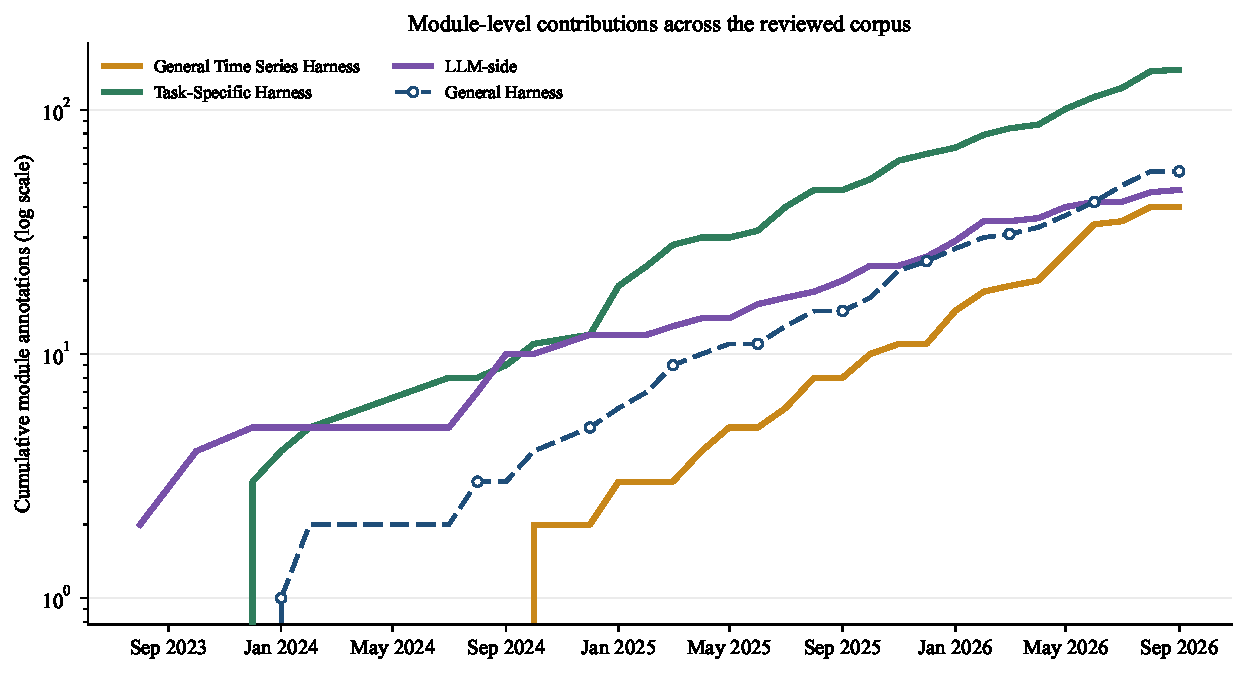
\includegraphics[width=\linewidth]{artifacts/contribution_timeline.pdf}
\caption{Cumulative module annotations in the maintained corpus, including reviewed modules and candidate classifications. Each reviewed module is counted once at its assigned layer, independently of its number of mechanism or task labels. The logarithmic axis makes early annotations visible; dashed lines and hollow markers identify General Harness.}
\label{fig:contribution-trend}
\end{figure}

\subsection{Position relative to existing surveys}

Existing surveys cover important subsets of the landscape. Task-oriented surveys discuss forecasting, change-point detection, anomaly detection, and deep architectures from their respective methodological perspectives \citep{aminikhanghahi2017changepoint,lim2021deepts,darban2024anomaly}. Surveys on time-series foundation models, synthetic data, LLM integration, and multimodal temporal modeling summarize pretraining, adaptation, serialization, prompting, tokenization, cross-modal alignment, data generation, and evaluation \citep{liang2024foundation,liu2025synthetic,zhang2024llmts,jiang2024empowering,liu2025crossmodality,jiang2025multimodal}.

Among the closest related surveys, \textit{From Prompts to Agents: A Comprehensive Survey of LLM-Driven Time Series Analysis} \citep{promptstoagents2026} separates representation, model adaptation, workflow autonomy, and analytical tasks; its workflow-autonomy axis further distinguishes predictor, augmenter, orchestrator, and multi-agent-collaboration levels, while the survey also discusses perception, planning, tool use, memory, and reflection. \textit{A Survey of Reasoning and Agentic Systems in Time Series with Large Language Models} \citep{changsurvey2026} describes reasoning topologies, objectives, and mechanism tags. \textit{LLM Agents for Time-Series: A Survey} \citep{chen2026tsagentsurvey} organizes the task-facing literature into forecasting and reasoning, augmentation and synthesis, anomaly detection and diagnosis, and decision support. These surveys supply the component and task vocabularies from which our framework is built. Harness literature defines the Agent runtime; time-series task structure determines whether a temporal mechanism is cross-task or task-specific. Our contribution is the resulting hierarchical organization.

Several system and position papers motivate this runtime perspective. ATSF frames forecasting as an iterative perception--planning--action--reflection--memory process \citep{atsf2026}. AION formalizes time-series tasks through task files, workspaces, validation interfaces, artifacts, and layered review \citep{aion2026}. TimeClaw implements a time-series-native runtime with executable tools, episodic multimodal memory, auditable trajectories, and experience-driven capability evolution \citep{timeclaw2026harness}. We organize these systems by the runtime layer each work changes and connect reusable temporal mechanisms to task-specific workflows and temporal design requirements.

\begingroup
\scriptsize
\setlength{\tabcolsep}{3.5pt}
\renewcommand{\arraystretch}{1.15}
\noindent\textbf{How to read the comparison.} This table asks what each time-series-agent survey chooses as its organizing object and what that choice lets the survey answer. A checkmark means that the dimension is explicitly developed in the cited survey; blank cells indicate that the dimension is outside its stated scope. The pattern motivates our contribution-locus view: model capability, task organization, workflow, lifecycle, process evaluation, and deployment utility can be read together rather than as isolated vocabularies.
\begin{longtable}{L{\fulltextcol{0.19}} C{\fulltextcol{0.09}} C{\fulltextcol{0.12}} C{\fulltextcol{0.12}} C{\fulltextcol{0.12}} C{\fulltextcol{0.12}} C{\fulltextcol{0.12}} C{\fulltextcol{0.12}}}
\caption{Discriminative dimensions across time-series-agent surveys. Columns shared by all surveys are omitted; checkmarks indicate explicit coverage. Sources: \citep{promptstoagents2026,changsurvey2026,chen2026tsagentsurvey,xu2026forecastagentsurvey}.}\label{tab:direct-prior-comparison}\\
\toprule
\textbf{Survey} & \textbf{Model} & \textbf{Tasks} & \textbf{Reasoning} & \textbf{Lifecycle} & \textbf{Coverage} & \textbf{Evaluation} & \textbf{Deployment}\\
\midrule
\endfirsthead
\toprule
\textbf{Survey} & \textbf{Model} & \textbf{Tasks} & \textbf{Reasoning} & \textbf{Lifecycle} & \textbf{Coverage} & \textbf{Evaluation} & \textbf{Deployment}\\
\midrule
\endhead
\textit{From Prompts to Agents: A Comprehensive Survey of LLM-Driven Time Series Analysis} \citep{promptstoagents2026} & \no & \yes & \yes & \no & \yes & \yes & \no\\
\textit{A Survey of Reasoning and Agentic Systems in Time Series with Large Language Models} \citep{changsurvey2026} & \no & \no & \yes & \no & \no & \yes & \no\\
\textit{LLM Agents for Time-Series: A Survey} \citep{chen2026tsagentsurvey} & \yes & \yes & \yes & \no & \yes & \yes & \no\\
\textit{LLM-Based Agents for Forecasting and Prediction: Methods, Training, Evaluation, and Applications} \citep{xu2026forecastagentsurvey} & \yes & \yes & \yes & \yes & \no & \yes & \yes\\
\midrule
\textbf{Ours} & \yes & \yes & \yes & \yes & \yes & \yes & \yes\\
\bottomrule
\end{longtable}
\endgroup

\noindent\textit{Reading the table.} The table retains the dimensions that separate the compared surveys. Our survey spans the full set by linking model-side contributions, task organization, reasoning and workflow, system lifecycle, multi-task coverage, agent-process evaluation, and deployment-oriented decision utility.


\textit{LLM-Based Agents for Forecasting and Prediction: Methods, Training, Evaluation, and Applications} \citep{xu2026forecastagentsurvey} organizes LLM-based forecasting and prediction agents around standalone LLMs, tool- and retrieval-augmented systems, and hybrid systems, while connecting methods to training, evaluation, applications, and risks. Its organizing unit is the forecasting/prediction system and its lifecycle; ours is the contribution locus of the underlying Harness. Its three system types map naturally to GH, GTS, and TSK components at different Harness depths, with each component assigned to its deepest applicable layer.

We re-read the broader literature through this additional contribution-locus question. Tools, memory, multimodality, decomposition, verification, and agent loops recur across the literature. We synthesize them into a seven-dimension \GeneralHarness{} comparison vocabulary from General Harness architecture, engineering, and agent-survey studies \citep{ning2026codeharness,lee2026metaharness,lin2026agenticharness,changsurvey2026,chen2026tsagentsurvey,xu2026forecastagentsurvey}. The dimensions form a common comparison layer; temporal obligations and the primary-locus rule provide the domain-specific coding and evaluation lens.

\subsection{Contributions}

This survey makes five contributions.

\begin{enumerate}
  \item We give a construction view of Time-Series Agents: a scenario becomes a task contract, the contract selects a General Harness, temporal obligations add a Time-Series Harness Module, and a task-specific module completes the system.
  \item We separate LLM-side capabilities from the nested Harness layers, distinguishing reusable runtime mechanisms, cross-task temporal mechanisms, and mechanisms bound to one task contract.
  \item We provide a module-level evidence ledger in the appendix. Each Paper Card records a work's claim, source locator, contribution modules, task contract, evaluation evidence, and review status so that future systems can be added without changing the organizing coordinates.
  \item We define an evaluation path that follows the construction: General Harness process, temporal contract, task outcome, resource behavior, and decision utility. The benchmark chapter maps existing resources to these evaluation layers.
  \item We derive open problems from missing interfaces and weakly evaluated contracts, including temporal faithfulness, provenance, self-evolution, reproducibility, and decision-centric evaluation.
\end{enumerate}

\noindent\textbf{How the paper is organized.} This map is a reading guide for the whole survey. Follow the arrows from the LLM side and reusable runtime to temporal contracts, task modules, evaluation, and open problems; the sequence mirrors the construction process of a Time-Series Agent. Its purpose is to show why the later sections are not a list of methods: each section answers the next design or evaluation question.

\begin{figure}[htbp]
\centering
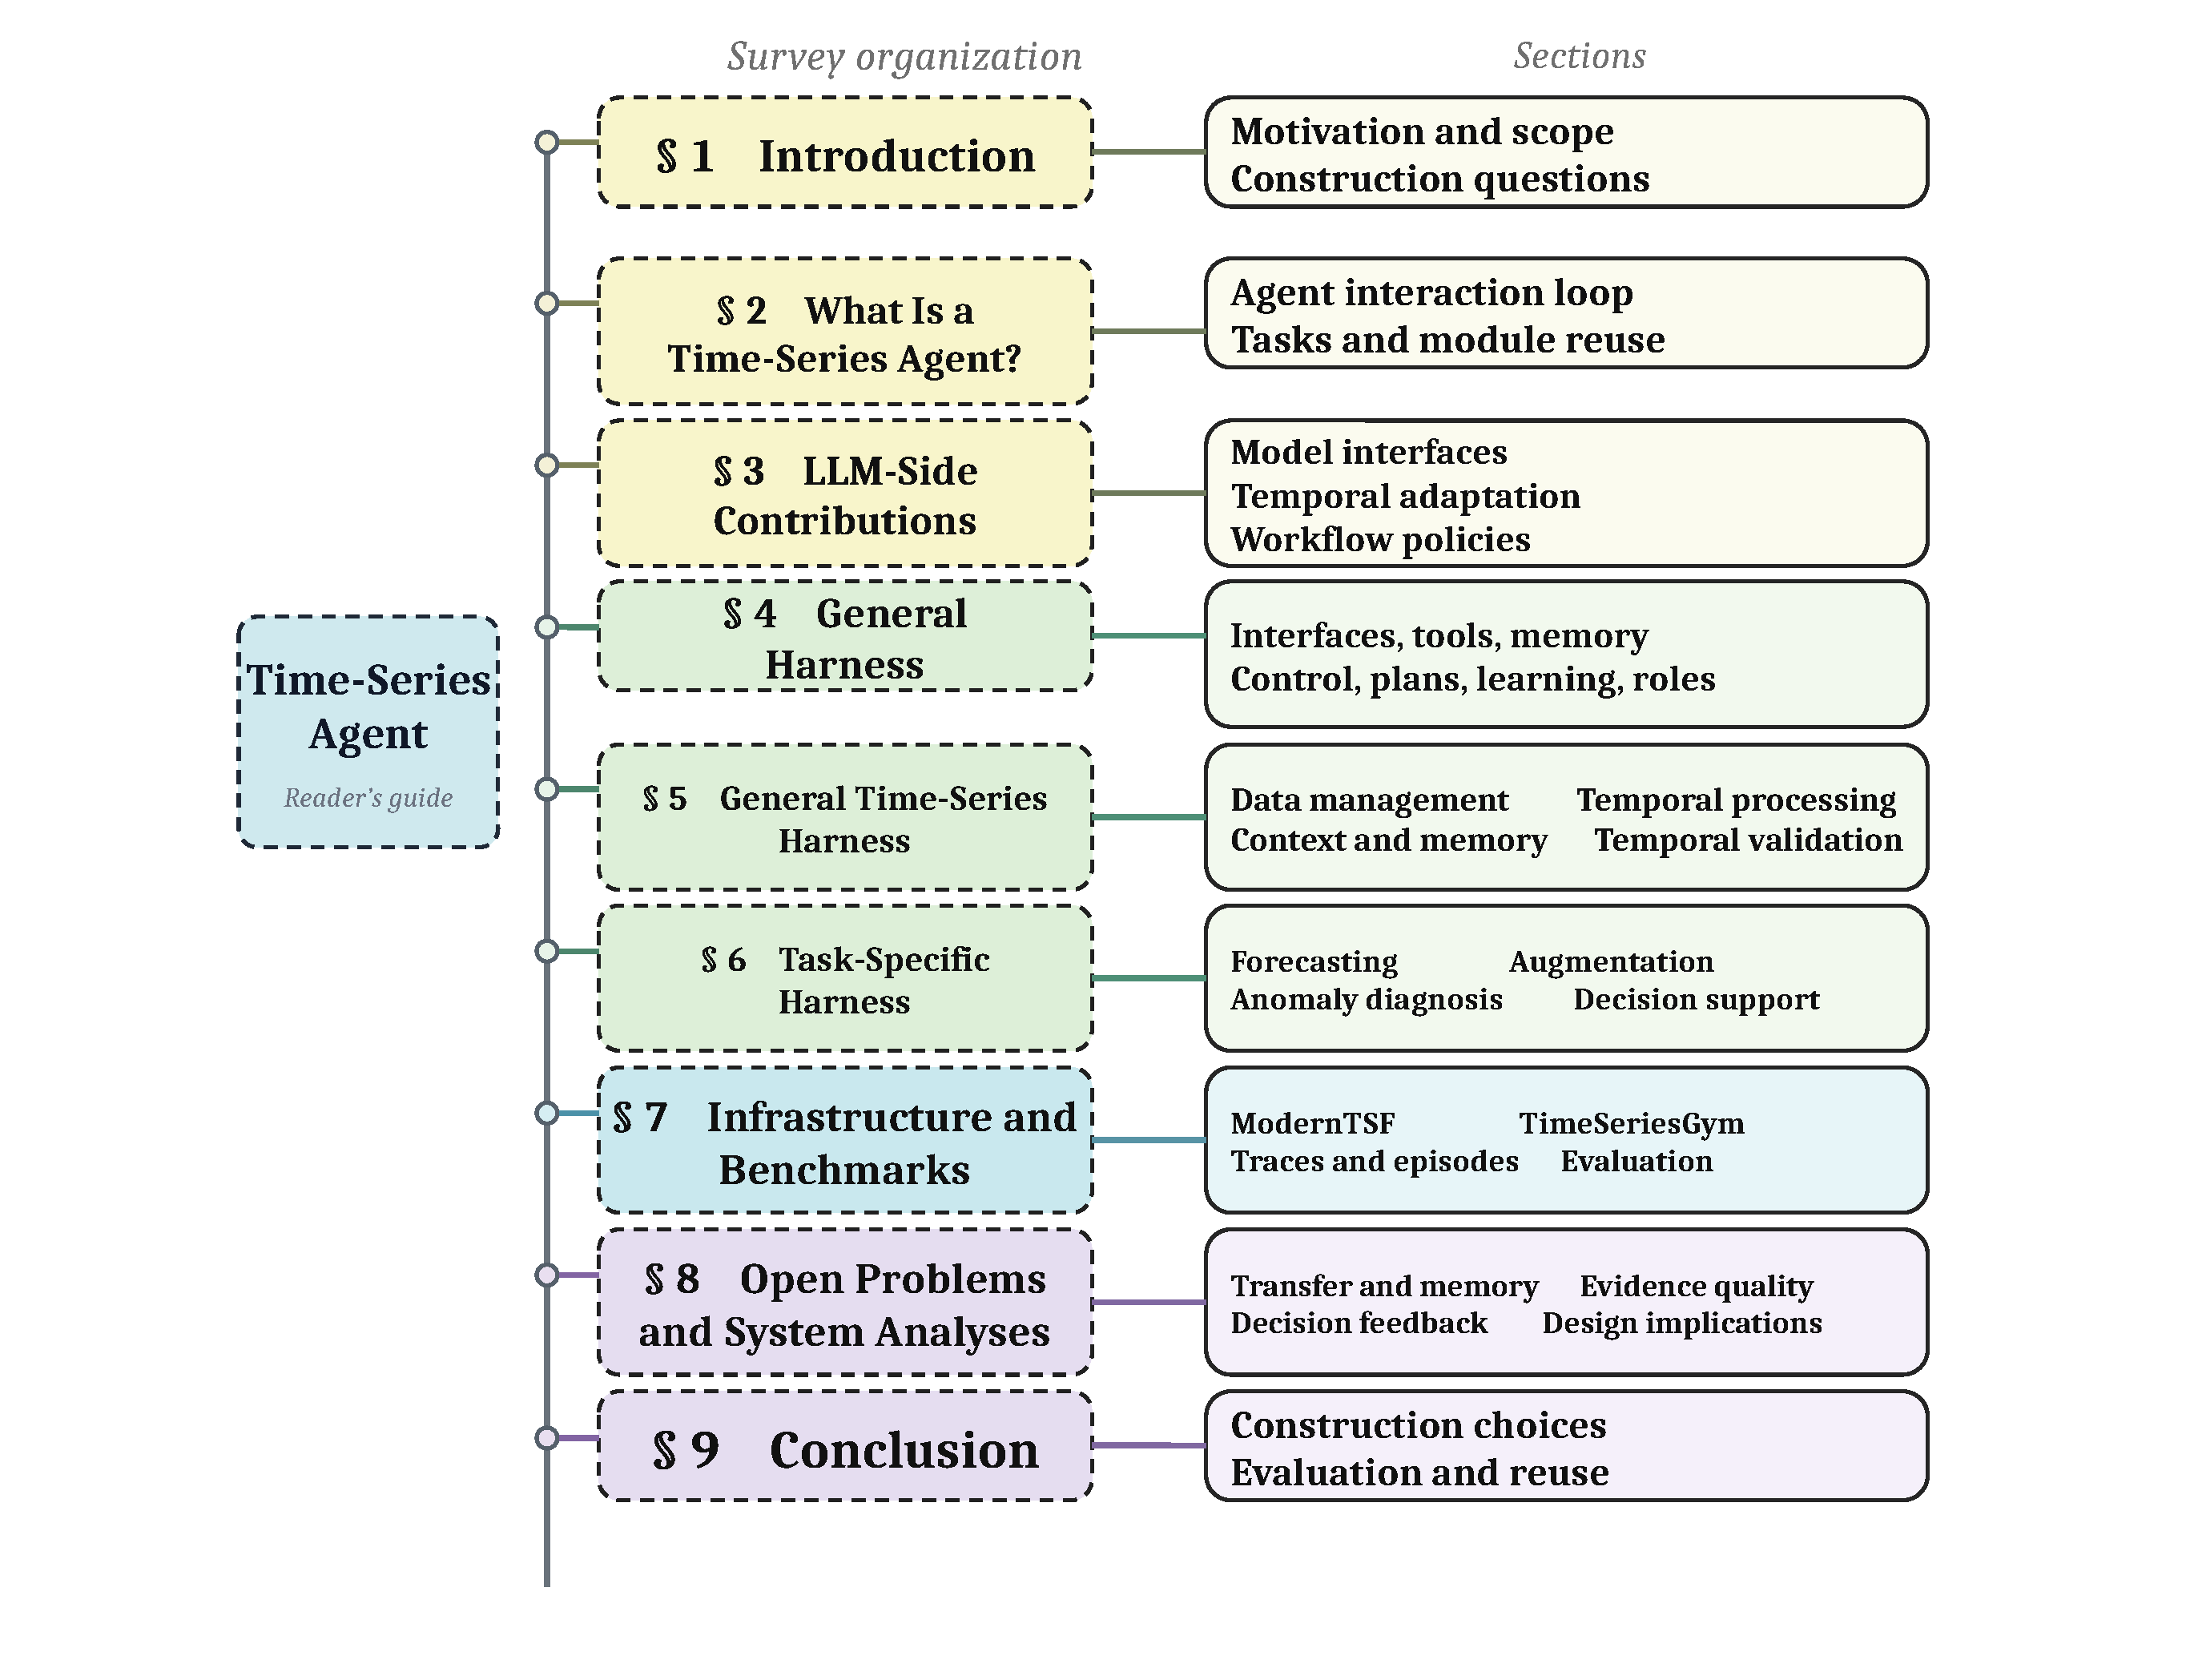
\includegraphics[width=\linewidth]{artifacts/active/Figure2_organization_rsi_adapted.pdf}
\caption{Organization of the survey. The sections follow the construction of a Time-Series Agent, from the LLM side and reusable runtime to temporal contracts, task modules, evaluation, and open problems. The module-level ledger provides the evidence record behind each section. The editable source is adapted from the RSI-style survey template and the labels and hierarchy are rewritten for this survey.}
\label{fig:survey-organization}
\end{figure}

\noindent\textbf{How to read the construction diagram.} The left branch is the independent LLM-side contribution; the nested right branch shows increasing temporal and task specificity. A mechanism moves downward only when its temporal state, operation, or validator becomes less reusable. This figure supplies the hierarchy used in the subsequent sections and in the exclusive module-level statistics.

\begin{figure}[H]
\centering
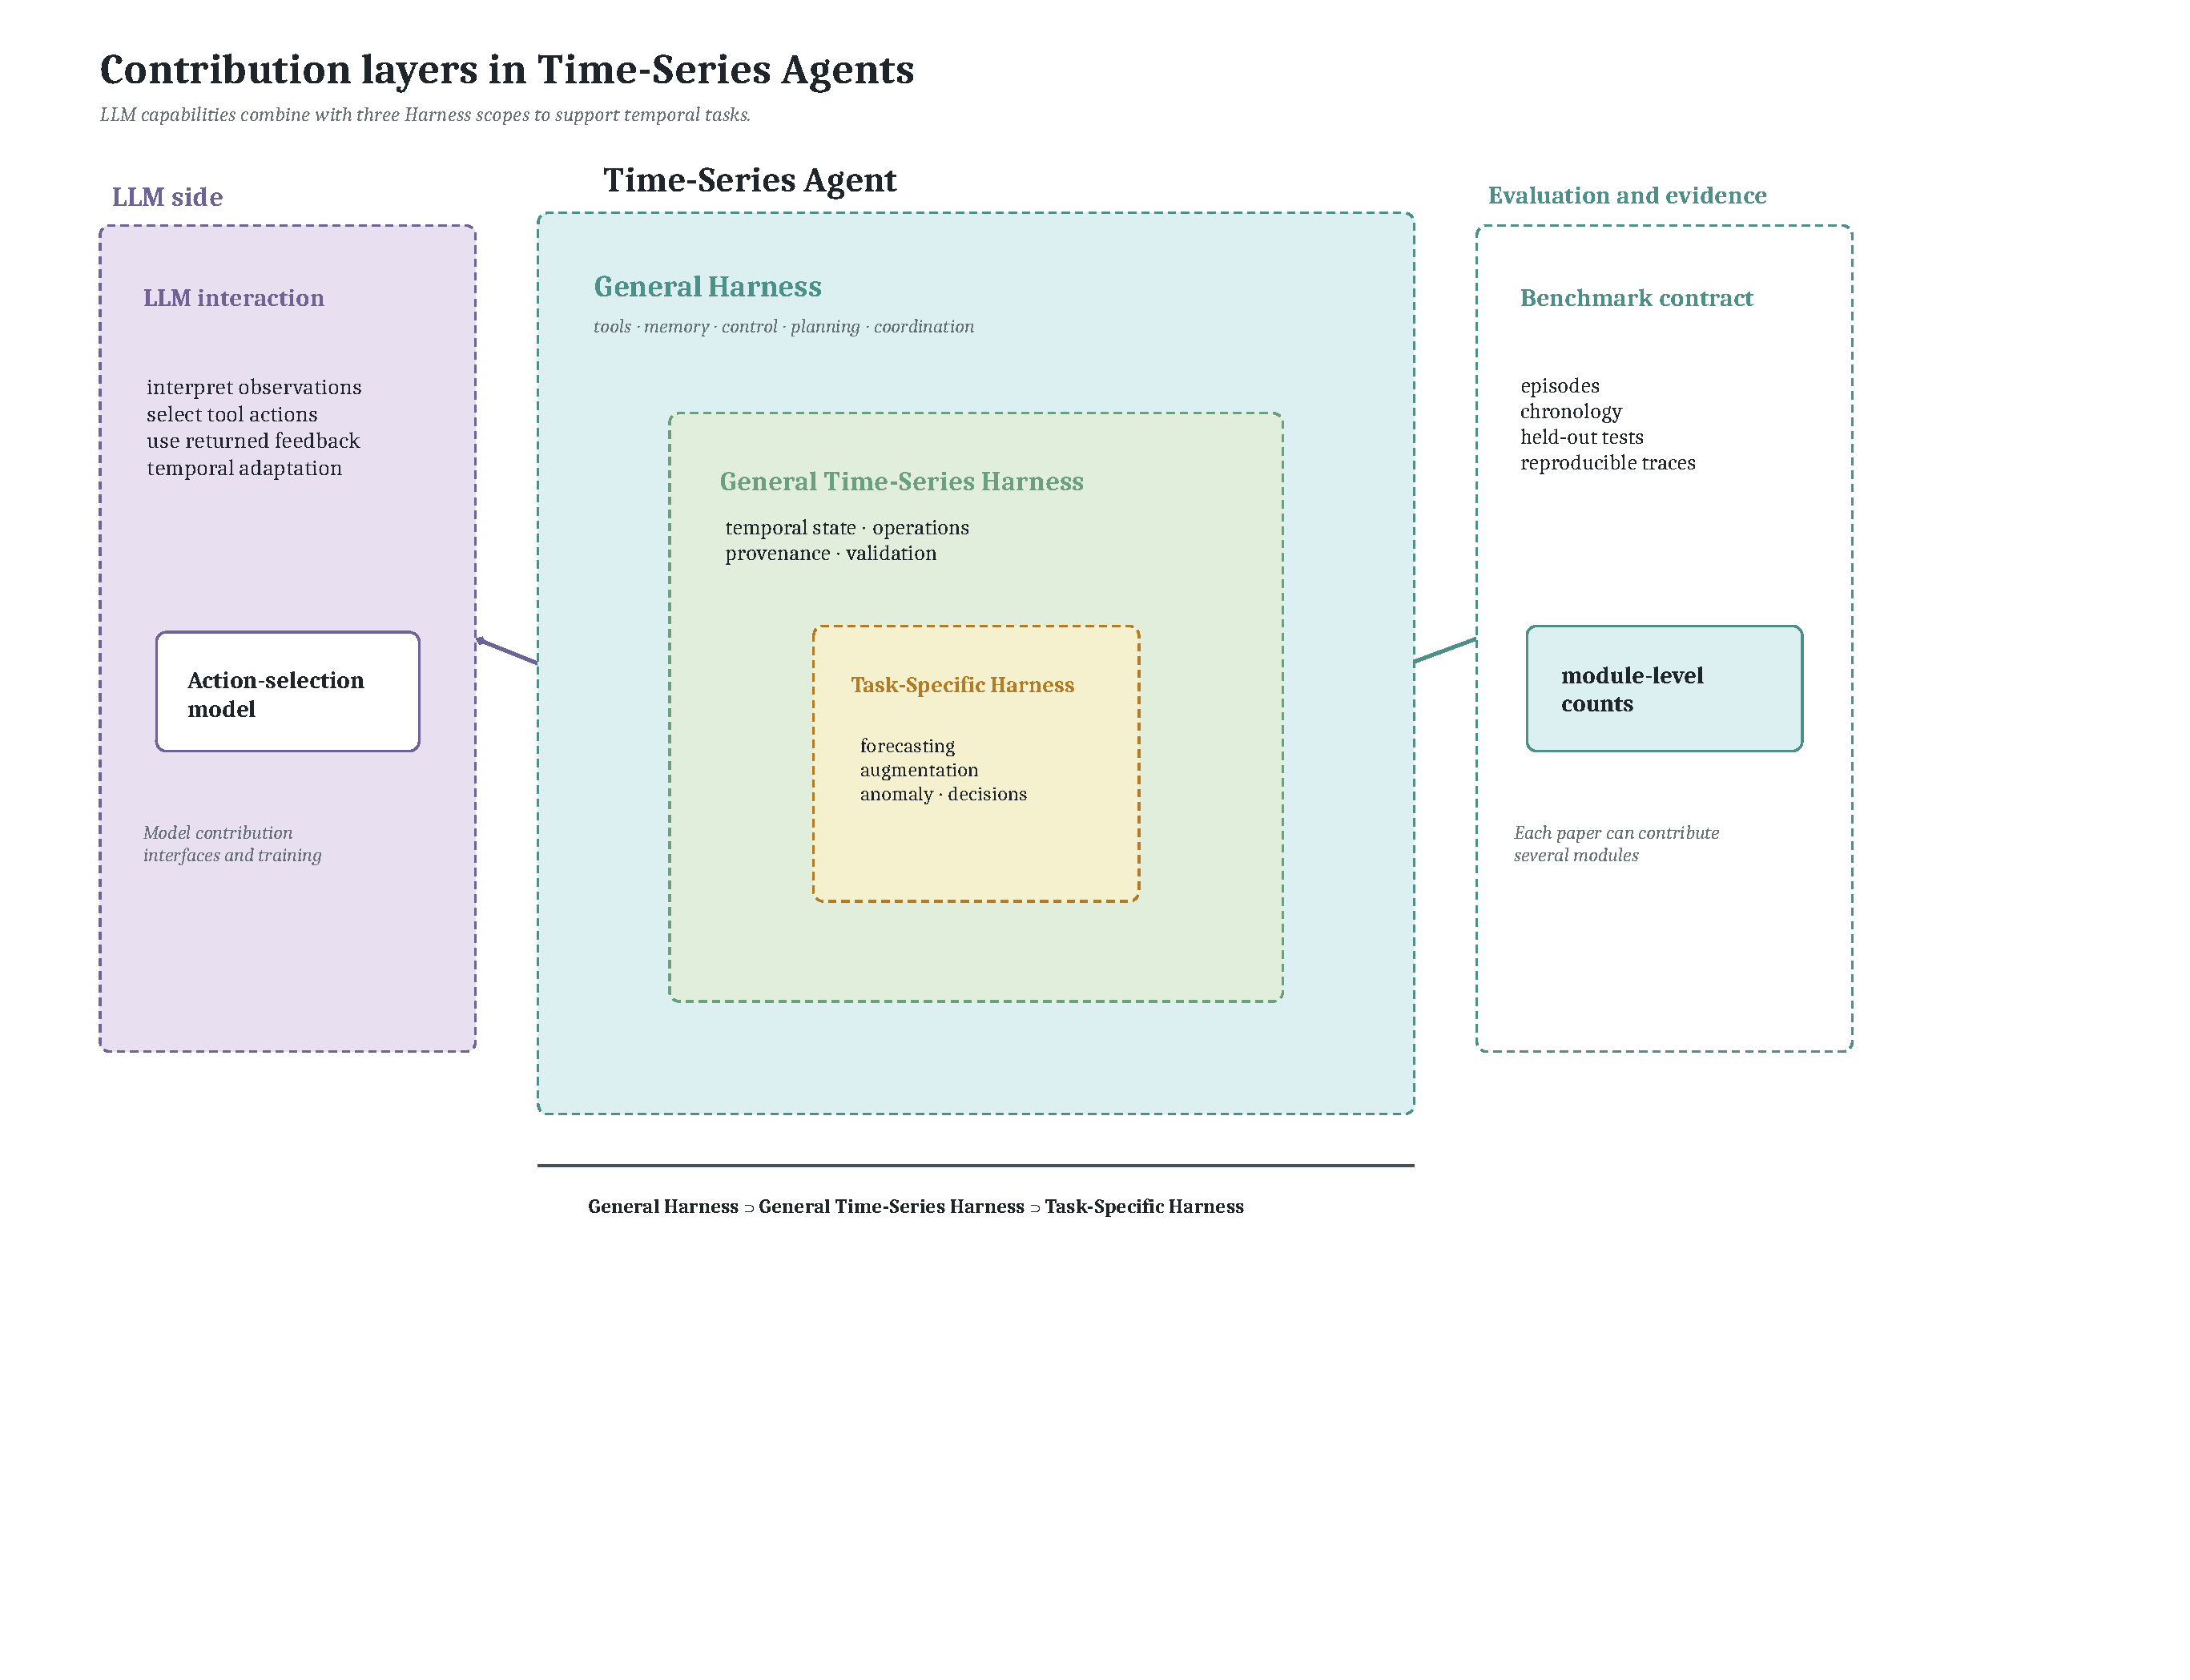
\includegraphics[width=\linewidth]{artifacts/active/Figure3_construction_rsi_adapted.pdf}
\caption{Contribution layers in a Time-Series Agent. The LLM side remains independent of the nested Harness stack: General Harness contains reusable runtime mechanisms, General Time-Series Harness contains temporal mechanisms that transfer across tasks, and Task-Specific Harness instantiates a task contract. The evaluation and ledger panel records how module-level evidence is counted. The editable source is adapted from the RSI-style survey template and rewritten for this survey.}
\label{fig:overview}
\end{figure}


\section{What Is a Time-Series Agent?}

A Time-Series Agent is a system in which an LLM operates through a reusable runtime and time-series-specific modules.

The LLM supplies language understanding and reasoning. The General Harness supplies interaction, memory, tools, execution, control, planning, optimization, and coordination. The Time-Series Harness Module preserves temporal state, operations, context, and validation; statistical models, time-series foundation models, databases, simulators, retrieval systems, and evaluators operate as callable components within it.

At an abstract level, the runtime can be written as
\begin{equation}
  a_t = \pi_\theta(s_t), \qquad
  s_{t+1} = \mathcal{H}(s_t,a_t,o_{t+1}),
  \label{eq:agent-loop}
\end{equation}
where $s_t$ is the visible state, $a_t$ is a tool or environment action, $o_{t+1}$ is the returned observation, and $\mathcal{H}$ is the Harness transition. Time-Series Harness Modules add temporal type information to each state, action, and observation.

We describe each contribution using one set of coordinates: its LLM or Harness locus, its mechanism, and its task. LLM-side contributions change the model's temporal capabilities. A Harness module receives one scope: General Harness for domain-independent execution, General Time-Series Harness for reusable temporal functionality, or Task-Specific Harness for a procedure tied to a task output or objective. The seven mechanism dimensions in Table~\ref{tab:component-vocab} apply throughout the Harness chapters. Task labels describe the outputs supported by a module. A paper may contribute several modules, and a module may have several mechanism or task labels while contributing one unit to its assigned layer.

The construction begins with the scenario, not with a model name. A scenario specifies the data stream, the information boundary, the operational objective, the allowed actions, and the evidence needed for review. Its task contract specifies the output object, temporal horizon, constraints, metric, and authority to accept, revise, or escalate the result. This contract determines which parts of the Harness must be temporal and which can remain general.

\begin{enumerate}
  \item \textbf{Specify the scenario.} State the data sources, event and availability times, channels, units, missingness policy, and the decision or analysis that follows the output.
  \item \textbf{Write the task contract.} Define the output, horizon, admissible information, constraints, evaluation metric, and review authority.
  \item \textbf{Select the runtime.} Choose General Harness mechanisms for interaction, memory, tools, execution, control, planning, optimization, and coordination.
  \item \textbf{Add temporal semantics.} Introduce temporal state, operations, provenance, chronology guards, and validators wherever a generic runtime leaves the meaning ambiguous.
  \item \textbf{Instantiate and evaluate.} Add task-specific modules, then evaluate process validity, temporal validity, task performance, resource use, failures, revision, and downstream decision utility.
\end{enumerate}

This sequence is the practical meaning of the survey's hierarchy. The same runtime can support financial forecasting, traffic prediction, industrial diagnosis, or demand planning; the temporal and task contracts determine which modules and benchmarks must change.

To keep the method descriptions comparable, we use the following notation throughout the survey. The table records symbols that recur in the method descriptions and in the paper-card ledger. The applicable-layer field is descriptive; module counts still use the deepest-applicable-layer rule stated above.

\begin{table}[htbp]
\centering\small
\setlength{\tabcolsep}{4pt}
\renewcommand{\arraystretch}{1.12}
\noindent\textbf{Notation used by the method descriptions.} The table fixes the symbols that recur in equations across the survey so that each method can be compared at the same level: temporal data and information sets, actions and observations, Harness layers, and task contracts. It is a reference table rather than a taxonomy; readers can return to it when a later method introduces a new training objective or evaluation variable.
\begin{tabularx}{\linewidth}{@{}p{0.18\linewidth}p{0.31\linewidth}p{0.18\linewidth}X@{}}
\toprule
\textbf{Symbol} & \textbf{Meaning} & \textbf{Applicable layer(s)} & \textbf{Use}\\
\midrule
$x_{1:T}$ & Multivariate time series with $T$ observations, channels, units, and timestamps. & LLM / GTS & Input to representation, temporal operations, and task modules.\\
$t,\tau,H$ & Event time, decision or forecast-origin time, and forecast horizon. & GTS / TSK & Define chronological availability and task output intervals.\\
$\mathcal{I}_{\tau}$ & Information admissible at time $\tau$, including availability and provenance. & GTS & Governs retrieval, memory, validation, and leakage control.\\
$s_k,a_k,o_{k+1}$ & Agent state, action or tool call, and returned observation at step $k$. & GH & Describe the reusable state--action loop.\\
$\omega_k$ & Typed tool call: name, arguments, permissions, budget, and failure contract. & GH / GTS & Makes execution and temporal arguments inspectable.\\
$\mathcal{M}_{\tau}$ & Memory available at $\tau$ with time index, vintage, provenance, and revision status. & GH / GTS & Defines point-in-time retrieval and experience reuse.\\
$\mathcal{V}$ & Validator or verifier that returns a pass, fail, finding, or escalation decision. & GH / GTS / TSK & Checks process, temporal, and task-specific obligations.\\
$\mathcal{C}_{\mathrm{task}}$ & Output contract for forecasting, augmentation, anomaly diagnosis, or decision support. & TSK & Specifies the object, metric, constraint, and review authority.\\
$(\widehat{y},\widehat{z},\widetilde{x},a^{\star})$ & Forecast, anomaly decision, generated series, and selected action. & TSK & The four representative task outputs used in Section~6.\\
\bottomrule
\end{tabularx}
\caption{Unified notation for the module-level method descriptions. GH denotes General Harness, GTS denotes General Time-Series Harness, and TSK denotes Task-Specific Harness.}
\label{tab:unified-notation}
\end{table}



The rest of the survey follows these construction layers. Section~3 isolates changes to the LLM; Section~4 describes the General Harness; Section~5 identifies the parts that become genuinely time-series-specific; Section~6 instantiates them under four task families; and Section~7 evaluates the resulting systems and the infrastructure needed to benchmark them.
\section{LLM-Side Contributions for Time-Series Agents}

The LLM is one of the three principal construction layers in a Time-Series Agent. This section records work that changes the model's ability to represent, align, understand, or reason about temporal data. The surrounding Harness is discussed in the following sections.

\subsection{Temporal representation and alignment}

\begin{figure}[htbp]
\centering
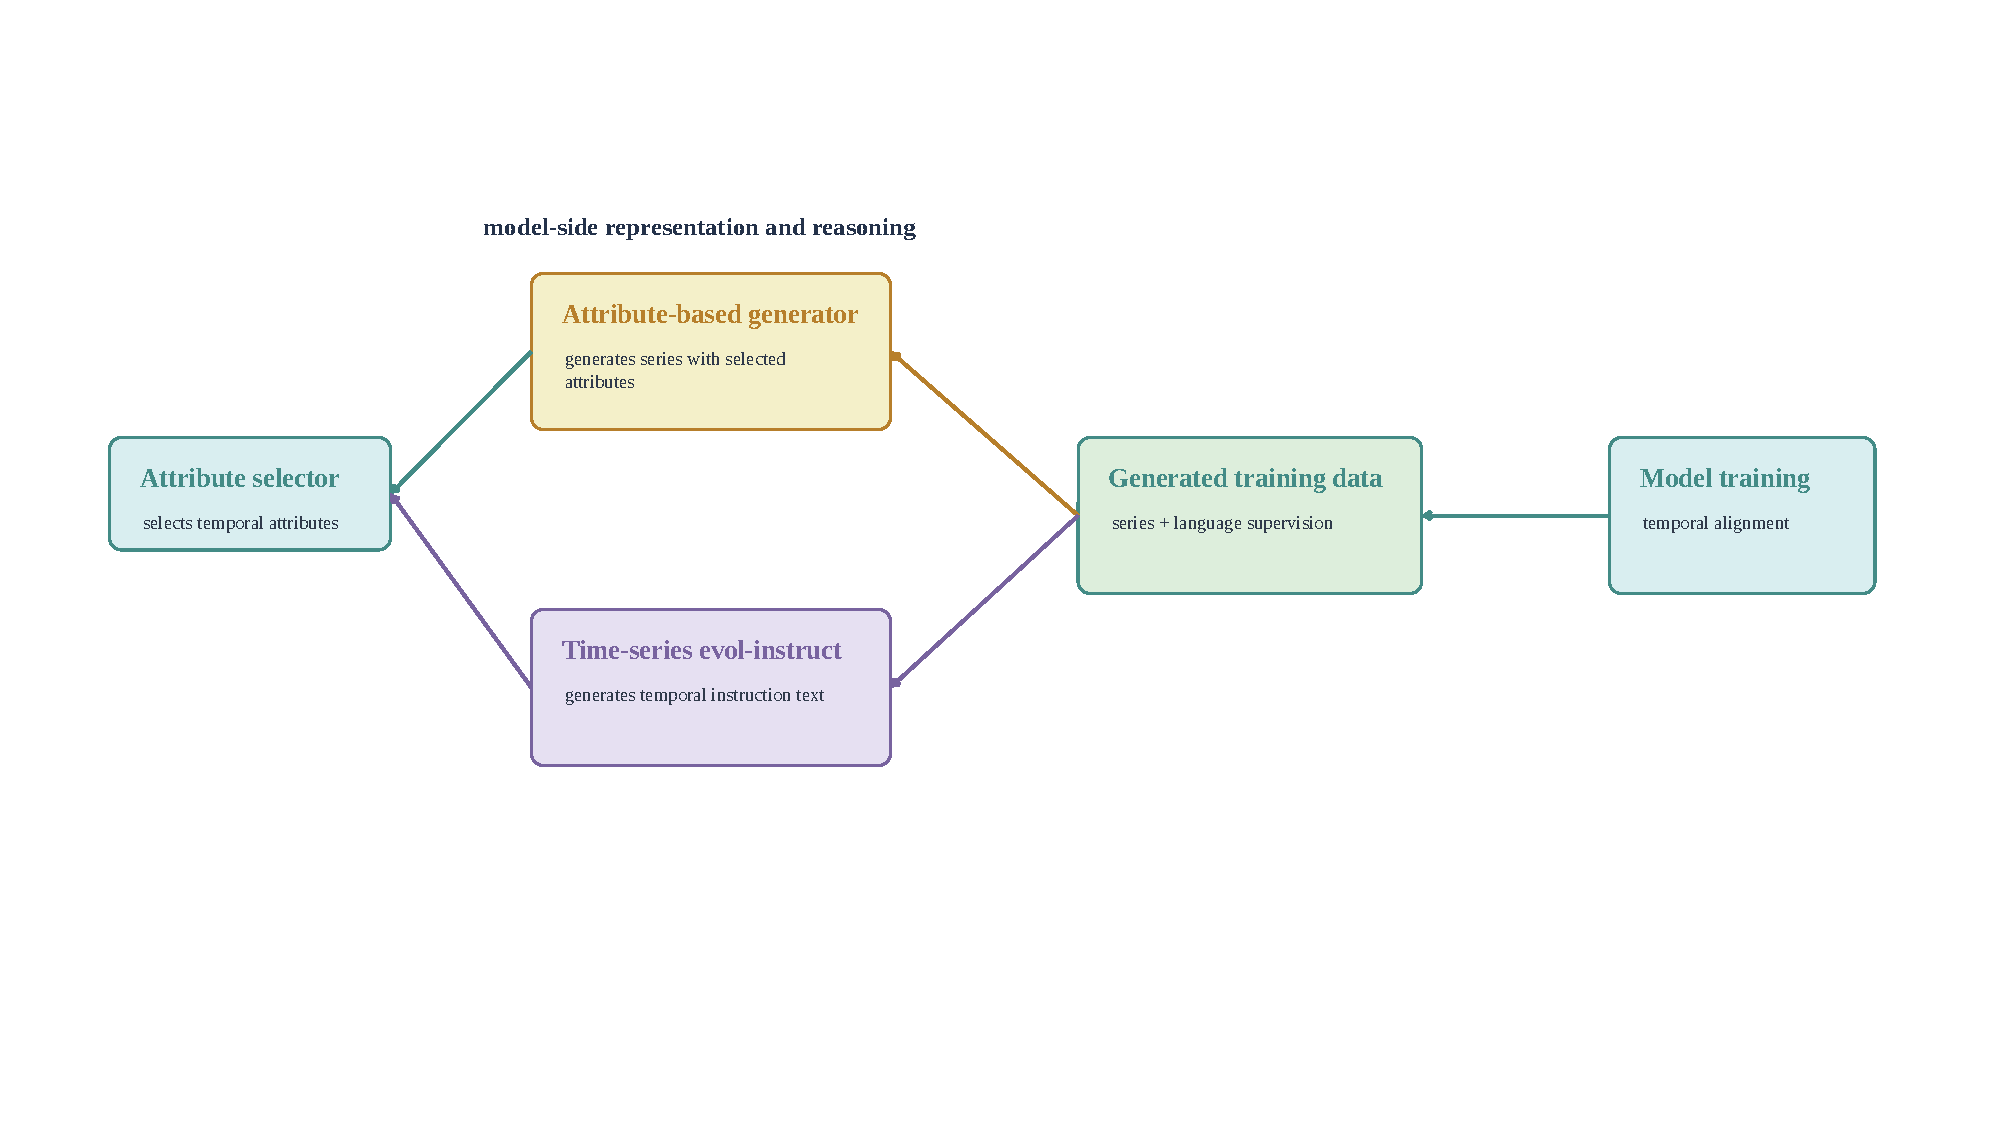
\includegraphics[width=0.78\linewidth]{artifacts/active/support_pdf/chatts_overview_native.pdf}
\caption{The temporal alignment pipeline makes the LLM-side interface visible: numerical values and temporal attributes are converted into language-facing supervision before any Harness tool is called. Source: \citep{chatts2025}.}
\label{fig:llm-alignment}
\end{figure}


These methods change how an LLM receives temporal values. Time-LLM reprograms a frozen language model with text prototypes and a Prompt-as-Prefix context, while LLM4TS aligns a pretrained language model with time-series inputs for data-efficient forecasting \citep{jin2024timellm,chang2024llm4ts}. Multimodal systems extend the same model-side boundary to visual or textual temporal context \citep{timevlm2025,timeomnivl2026}. Conversational Time Series Foundation Models place the LLM in the role of an ensemble judge: the model interprets temporal evidence, assigns weights to foundation forecasters, and explains the resulting forecast in dialogue \citep{conversationaltsfm2025}. STRIDE instead injects distilled reasoning into a continuous TSFM representation, coupling language-side reasoning with numerical forecasting \citep{stride2026}.

Time-LLM makes the input and output contracts explicit: for a multivariate series $X\in\mathbb{R}^{N\times T}$, the model produces a horizon of predictions $\widehat{Y}\in\mathbb{R}^{N\times H}$ and is trained with
\begin{equation}
  \mathcal{L}_{\mathrm{MSE}}=\frac{1}{H}\sum_{h=1}^{H}\left\|\widehat{Y}_{h}-Y_{h}\right\|_{F}^{2}.
  \label{eq:timellm-objective}
\end{equation}
The method first transforms the series into the language-model interface, applies a frozen LLM with Prompt-as-Prefix context, and projects the hidden states back to the forecast space \citep{jin2024timellm}. This objective captures the model-side contribution: temporal representation is aligned with the forecast space and trained under an explicit prediction loss.

\subsection{Temporal instruction, interaction, and reasoning}

A second line teaches the model to discuss and reason over temporal evidence. ChatTS constructs synthetic time-series instruction data and time-series dialogue for understanding and reasoning \citep{chatts2025}. Its direct extension, Towards Time-Series Reasoning, combines a trainable temporal encoder with supervised reasoning traces for cross-domain perception and analysis \citep{chow2024tsreasoning}. These works make natural-language temporal interaction a learned model capability. The same model-side direction appears in open-ended forecasting: OpenForecaster trains reasoning models on automatically curated future-event questions with retrieval and reinforcement learning, while AURA-4B studies tool-use post-training and PPO in a chronological stock-price sandbox \citep{openforecaster2026,auraforecaster2026}. ChatTS also preserves numerical meaning during normalization by exposing the scale and offset in the text prompt. For a series value $x_t$, its value-preserved normalization can be written as
\begin{equation}
  x_t^{\mathrm{norm}}=\frac{x_t-x_{\min}}{x_{\max}-x_{\min}},\qquad
  x_t=(x_{\max}-x_{\min})x_t^{\mathrm{norm}}+x_{\min},
  \label{eq:chatts-value-preserved}
\end{equation}
so the LLM receives normalized patches together with the parameters required to recover the original numerical scale \citep{chatts2025}. For instruction records $(x_i,q_i,r_i)$, the model-side training objective is
\begin{equation}
  \mathcal{L}_{\mathrm{dialog}}(\theta)=-\sum_{i=1}^{N}\log p_{\theta}(r_i\mid x_i,q_i).
  \label{eq:llm-dialogue-objective}
\end{equation}
ChatTS instantiates this objective with synthetic temporal attributes, instruction data, and dialogue responses \citep{chatts2025}.

ChatAD \citep{chatad2026}, Section~4.2, combines LoRA-based supervised fine-tuning with TKTO preference optimization. Its feedback score $S$ becomes a soft preference weight, which mixes desirable and undesirable response losses:
\begin{equation}
 \alpha=\sigma\!\left(\kappa(S-\eta)\right),\qquad
 \mathcal{L}_{\mathrm{TKTO}}=\mathbb{E}_{(x,y,d)\sim\mathcal{D}}
 [\alpha\mathcal{L}_{D}(\pi_\theta,x,y)+(1-\alpha)\mathcal{L}_{U}(\pi_\theta,x,y)].
 \label{eq:chatad-tkto}
\end{equation}
The supervised stage teaches anomaly responses, and the preference stage develops reasoning and generalization. The model update is an LLM-side contribution; the agents constructing its training dialogues are described in the synthesis section.

CastFSR \citep{castfsr2026} also has a model-side variant: supervised distillation teaches the Fast--Slow--Reflect workflow, followed by multi-turn reinforcement learning over complete trajectories. The training checks tool calls, stage order, timestamps, and completed forecasts before optimizing forecasting feedback. This policy update is recorded separately from the runtime workflow described in Section~\ref{sec:task-specific-harness}.

The module ledger places learned data and reasoning under the LLM layer. Tool, memory, and validation contributions from the same work receive their own Harness entries, keeping multi-layer contributions visible.

\noindent\textbf{What the LLM-side figure establishes.} The diagram follows the ChatTS pipeline from temporal attribute selection to synthetic supervision and model training. It makes the LLM-side contribution concrete: the model is changed before the Harness chooses tools or controls execution. The redesign is based on the temporal alignment and instruction-data pipeline reported by ChatTS~\citep{chatts2025}; read it left to right as a sequence of learned interfaces.

\begin{figure}[htbp]
\centering
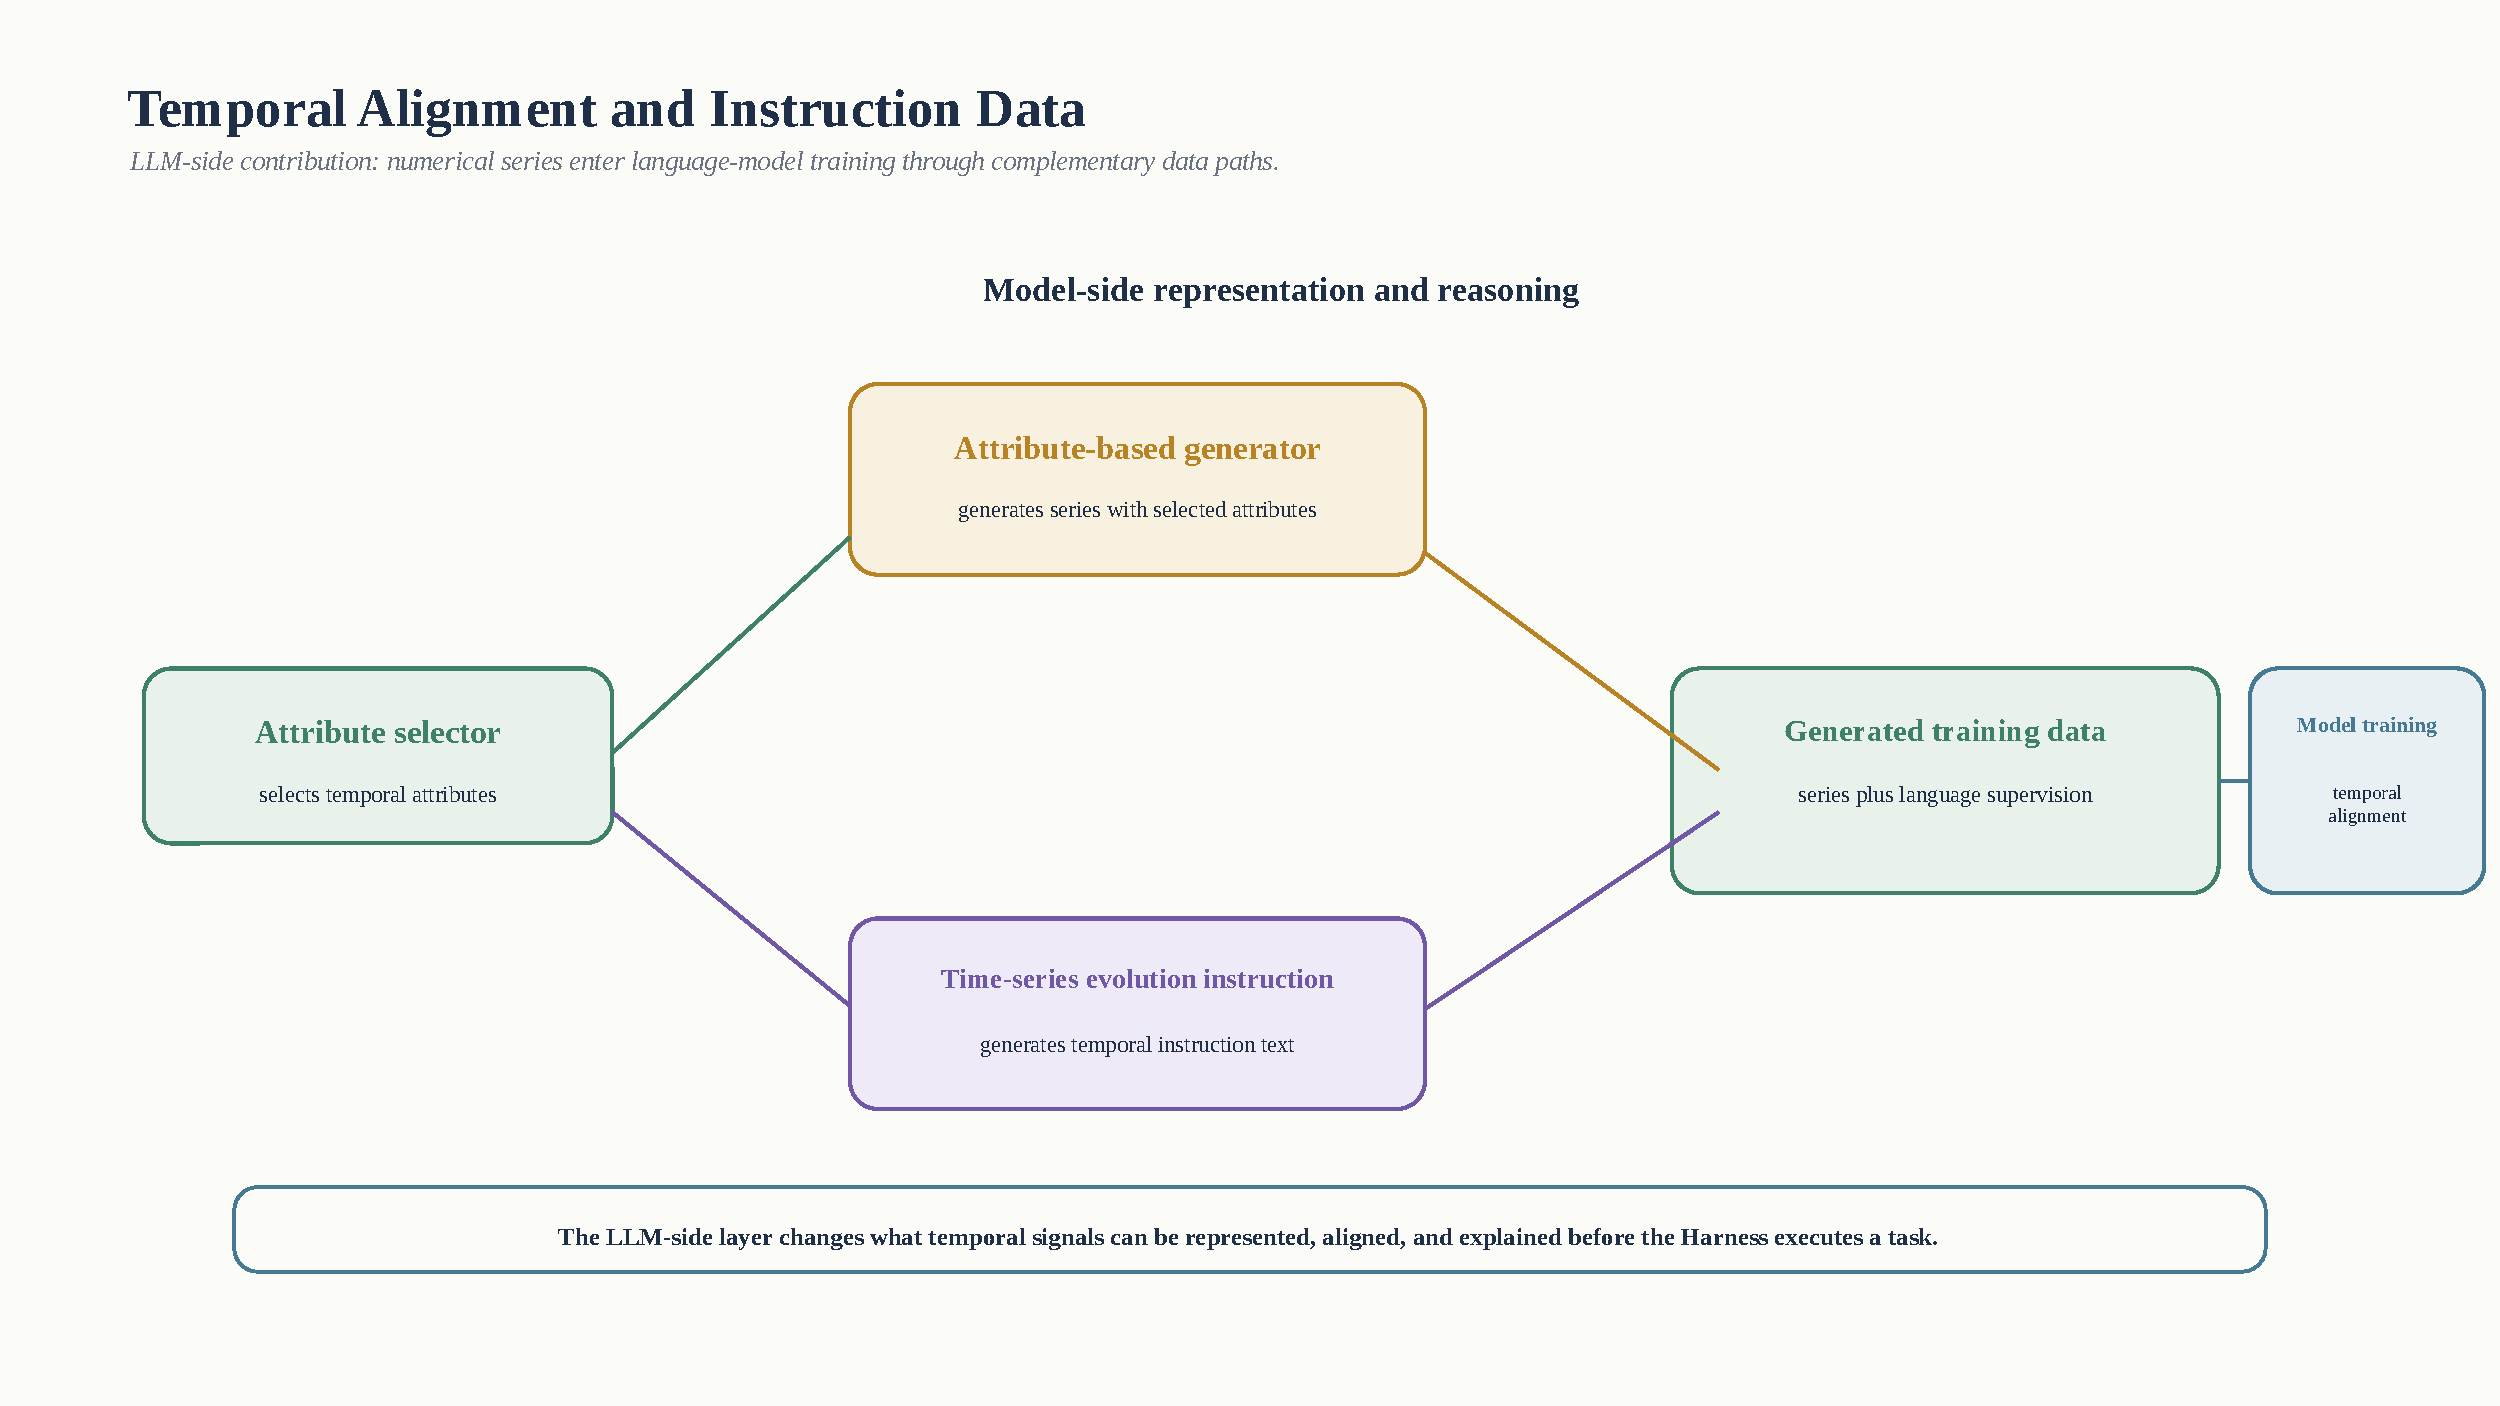
\includegraphics[width=0.88\linewidth]{artifacts/active/Figure_LLM_side_native_v3.pdf}
\caption{LLM-side temporal alignment and instruction data, adapted from the ChatTS training pipeline in Fig.~3 of \citet{chatts2025}. The editable map separates temporal attribute selection, synthetic supervision, instruction generation, and model training.}
\label{fig:chatts-overview}
\end{figure}

\subsection{LLM adaptation and the model-side boundary}

LLM-side adaptation includes continued training, parameter-efficient adaptation, temporal adapters, and task-specific supervision. Foundational studies such as LLMTime establish the capabilities and limits of serialized numerical inputs for language models \citep{gruver2023llmtime,tan2024useful,merrill2024struggle}. Adaptation methods update a temporal interface or a parameter-efficient module while preserving the base model:
\begin{equation}
  \theta_{\mathrm{adapt}}=\theta_{0}+\Delta_{\phi},\qquad
  \Delta_{\phi}^{\star}=\arg\min_{\Delta_{\phi}}\mathcal{L}_{\mathrm{TS}}(\theta_{0}+\Delta_{\phi}).
  \label{eq:llm-adaptation}
\end{equation}
We record model-side changes alongside any temporal tools, memory, or task contracts introduced by the same paper.

A stronger temporal encoder supplies the learned alignment and reasoning capability; a General Harness makes it callable; and a task-specific verifier checks the resulting forecast, diagnosis, or recommendation against its output contract. The module ledger records these changes as separate entries when a paper contributes to multiple layers.
\section{General Harness}
\label{sec:general-harness}

The General Harness is the reusable runtime around the LLM. In-scope systems instantiate or extend this runtime, while model-side and benchmark records provide complementary evidence. General Agent surveys provide the vocabulary and comparative basis for the seven dimensions \citep{ning2026codeharness,lee2026metaharness,lin2026agenticharness,changsurvey2026,chen2026tsagentsurvey,xu2026forecastagentsurvey}. Agent Cybernetics gives a systems-level account of reliability, lifelong operation, and self-improvement for tool loops, memory, harnesses, and reflection, which motivates the runtime dimensions used here \citep{agentcybernetics2026}.

Table~\ref{tab:component-vocab} states the seven-dimension domain-agnostic runtime vocabulary used in this survey. The dimensions synthesize recurring functions discussed across the Harness and agent surveys \citep{ning2026codeharness,lee2026metaharness,lin2026agenticharness,changsurvey2026,chen2026tsagentsurvey,xu2026forecastagentsurvey}; the same dimensions index the module evidence in the appendix.

\begingroup
\small
\setlength{\tabcolsep}{4pt}
\renewcommand{\arraystretch}{1.12}
\noindent\textbf{Purpose of the seven-dimension table.} This table is the shared comparison vocabulary for General Harness mechanisms. Each row answers one runtime question and names the operations included in that dimension; the rows can co-occur because one system can plan, call tools, preserve memory, and verify results in the same episode. The vocabulary is synthesized from the cited Harness and agent surveys~\citep{ning2026codeharness,lee2026metaharness,lin2026agenticharness,changsurvey2026,chen2026tsagentsurvey,xu2026forecastagentsurvey}.
\begin{longtable}{L{\fulltextcol{0.24}} L{\fulltextcol{0.30}} L{\fulltextcol{0.46}}}
\caption{A coarse-grained taxonomy of General Harness capabilities, synthesized from recurring functions in the General Harness and agent-survey literature \citep{ning2026codeharness,lee2026metaharness,lin2026agenticharness,changsurvey2026,chen2026tsagentsurvey,xu2026forecastagentsurvey}. The seven dimensions form an author-normalized comparison layer and can co-occur within one system.}
\label{tab:component-vocab}\\
\toprule
\textbf{Dimension} & \textbf{Question} & \textbf{Elements}\\
\midrule
\endfirsthead
\toprule
\textbf{Dimension} & \textbf{Question} & \textbf{Elements}\\
\midrule
\endhead
Interface and Interaction & How does the agent receive state and act on its environment? & Reasoning interfaces, action interfaces, environment modeling, user interaction, and state--action loops.\\
Memory and Context & How does the agent preserve and organize information across steps? & Context management, working and long-term memory, state stores, retrieval, and experience reuse.\\
Tools and Execution & How does the agent invoke external capabilities and execute actions? & Tool registries, APIs, retrieval, code execution, databases, forecasting models, and simulators.\\
Control, Verification, and Feedback & How does the agent detect errors, revise behavior, and assess reliability? & Control loops, error recovery, validators, feedback, review, evaluation interfaces, and observability.\\
Planning and Workflow & How does the agent organize multi-step work? & Task decomposition, planning, search, workflow orchestration, policy selection, and stopping conditions.\\
Optimization and Evolution & How does the agent or Harness improve from experience? & Prompt, tool, memory, policy, and Harness optimization; reflection and trajectory-driven evolution.\\
Coordination and Scaling & How do multiple agents divide work, communicate, and cooperate? & Role assignment, delegation, shared state, debate, review, and multi-agent orchestration.\\
\bottomrule
\end{longtable}
\endgroup

\noindent\textbf{Reading the General Harness figure.} The center is the runtime interface around an LLM; the seven surrounding nodes are reusable mechanism families, not seven mutually exclusive agent types. The figure supports the chapter's main claim: a Time-Series Agent can reuse these runtime mechanisms while temporal semantics are added in the next layer. The dimensions follow Table~\ref{tab:component-vocab}.

\begin{figure}[htbp]
\centering
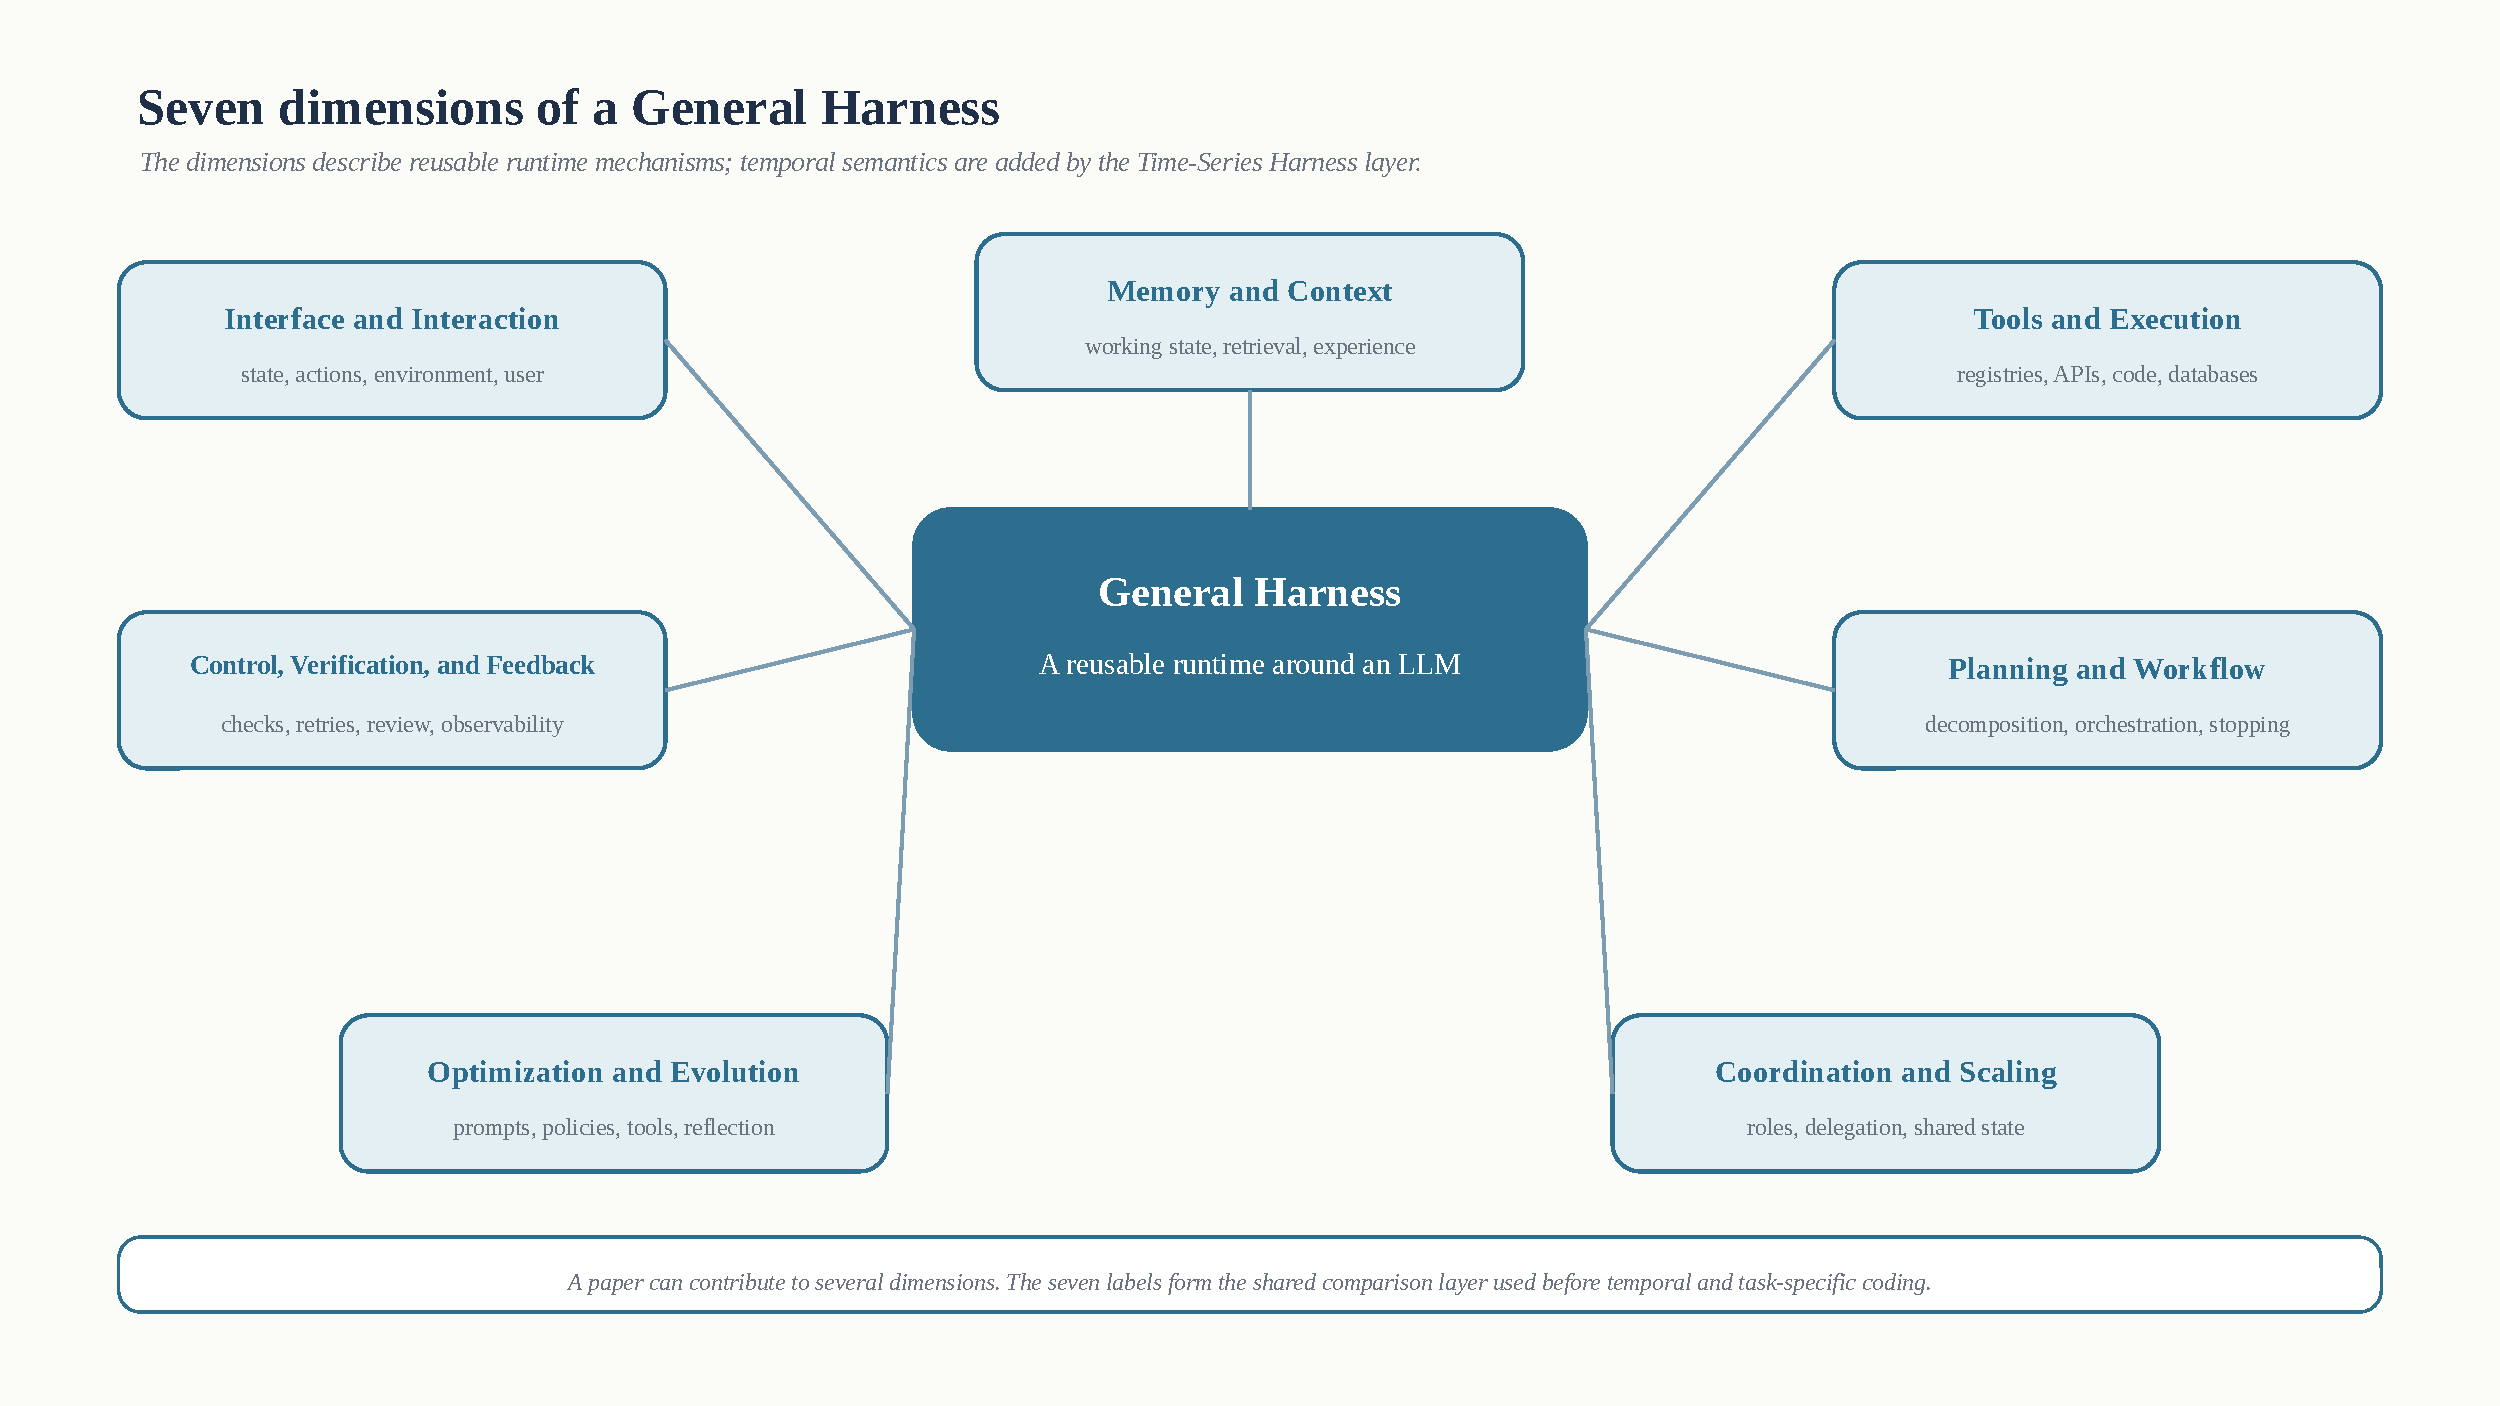
\includegraphics[width=0.96\linewidth]{artifacts/active/Figure4_general_harness_native_v2.pdf}
\caption{The seven reusable dimensions of a General Harness. The center represents the runtime around an LLM; each surrounding node is a mechanism family that can recur across domains. A paper may contribute to several dimensions, while temporal semantics are coded separately in the General Time-Series Harness layer.}
\label{fig:general-harness-seven-dimensions}
\end{figure}

The seven dimensions organize the evidence below. Each subsection first states the general mechanism and then points to its use in a Time-Series Agent. A work may instantiate any subset of these dimensions.

\subsection{Interface and Interaction}

An interaction interface specifies the request, visible state, available actions, and returned observations. TS-Agent \citep{tsagent2025} makes temporal questions actionable through analytical tools; TimeART \citep{timeart2026} and TSAG \citep{tsag2026} also connect language requests to structured analytical operations. The reusable part is the exchange protocol: the agent chooses an operation, receives its result or failure, and uses that observation in the next step. The operation's numerical meaning is supplied by the temporal or task-specific module.

For a new application, this boundary determines whether users provide an open-ended question, a structured task description, or a request requiring human confirmation. AION \citep{aion2026} represents the request through a task file, an accessible workspace, and a validation interface. Its task file declares the permissible output and constraints before execution begins. This makes the interface useful for both a forecast submission and an analytical report: the protocol is shared, while the required artifact changes.

\subsection{Memory and Context}

Memory supports continuity within an analysis and reuse across analyses. AION \citep{aion2026} records progress, decisions, and structural state so that review and execution can resume from a shared account of the work. This operational memory answers questions such as which files have been inspected, which candidate was tested, and why a previous step failed. Its organization can be reused across application domains.

MetaCaster \citep{metacaster2026} gives a concrete example of memory during optimization. Its Harness Proposer retains dataset snapshots, evaluation results, training logs, diagnoses, and update histories across epochs. These records support rollback and selection of a previous harness configuration. The storage and recovery mechanism belongs to General Harness; the forecasting error used to choose a configuration is developed in Section~\ref{sec:task-specific-harness}. TIMECLAW's signal-aware retrieval \citep{timeclaw2026harness}, in contrast, adds a temporal similarity criterion and is discussed with General Time-Series Harness memory.

\subsection{Tools and Execution}

A tool interface makes an external capability callable; the execution environment runs it and returns an observation. TimeCopilot \citep{timecopilot2025} exposes forecasting models, while TimeSeriesScientist \citep{timeseriesscientist2025} connects diagnostic, modeling, and reporting operations through specialized agents. The design question at this layer is how the runtime specifies arguments, dispatches work, captures artifacts, and reports failure. Model-selection objectives and temporal transformations are properties of the invoked procedures.

MetaCaster's Forecaster Trainer \citep{metacaster2026} illustrates the execution mechanism in detail. It assembles jobs indexed by forecaster, hyperparameters, and dataset, queues them, and assigns available GPUs. During execution it monitors processes, resolves errors, and recovers interrupted jobs until the queue is empty. Job scheduling and recovery can support other computational workloads; the selection of lightweight forecasters and their validation criteria supplies the task-specific part. Separating these two concerns makes it possible to reuse the executor while changing the analytical objective.

\subsection{Control, Verification, and Feedback}

Control determines what happens after an observation: continue, retry, request review, or finish. AION \citep{aion2026} separates validity checks from scored metrics and organizes review and stopping through explicit protocols. An agent can therefore produce a syntactically valid artifact that still requires substantive review, or obtain a good score while failing an admissibility check. This distinction is useful whenever tool execution, artifact acceptance, and task quality have different failure modes.

Feedback also has a timing requirement. Execution errors are available immediately; labels and downstream outcomes may arrive later. A forecast-error refinement procedure such as FLAIRR-TS \citep{flairr2025} uses observed target values as feedback and is explained in the forecasting section. A deployment must schedule that update when the corresponding outcomes are available. Evaluation conducted after an episode measures the procedure, whereas feedback available during the episode changes its actions.

\subsection{Planning and Workflow}

Planning selects the operations needed to produce a requested artifact and determines their dependencies. TimeSeriesScientist \citep{timeseriesscientist2025} organizes curation, planning, forecasting, and reporting into a four-agent workflow. Its intermediate analysis summary passes information about the input series to the model-selection stage, and the selected models and validation results then pass to the forecaster. This illustrates how a plan can be expressed through inspectable artifacts instead of an unrecorded chain of instructions.

AION \citep{aion2026} adds lifecycle rules and protocols that connect work, review, rechecking, memory updates, and stopping. For a new system, the important choice is which dependencies are fixed by the application and which the agent may revise. Data access and artifact acceptance can remain explicit checkpoints while the agent explores alternative analyses between them. The temporal content of those checkpoints is described in Section~\ref{sec:general-ts-harness}.

\subsection{Optimization and Evolution}

Optimization changes the prompts, procedures, or tools available to later executions. TIMECLAW \citep{timeclaw2026harness} implements a concrete tool-promotion loop: a code-specialized LLM receives clustered trajectories and task descriptions, extracts a recurring procedure, and produces an executable tool with an invocation description. The candidate runs on held-out similar tasks and joins the registry only when its success rate exceeds a threshold. The mechanism thus connects experience extraction, executable testing, and future reuse.

The promotion controller is reusable; each generated tool receives the scope appropriate to its own computation. A new temporal transformation can be a GTS module, while a forecast-specific revision routine is TSK. MetaCaster \citep{metacaster2026} illustrates an optimization loop whose scoring objective is explicitly tied to forecasting. Its method and objective are therefore developed alongside the forecasters and generated training data that they optimize.

\subsection{Coordination and Scaling}

Coordination specifies which agent performs each operation, what it shares, and who resolves disagreement. FinCon \citep{fincon2024} uses analyst roles and a manager to aggregate financial evidence; TimeSeriesScientist \citep{timeseriesscientist2025} passes outputs through curation, planning, forecasting, and reporting roles. These examples expose two reusable arrangements: evidence aggregation by a coordinator and staged delegation through a workflow.

AION \citep{aion2026} makes the communication boundary explicit through protocols for work, review, rechecking, stop signals, and memory updates. For implementation, this requires both the artifact being handed off and the condition under which the next role may act. Financial action constraints and forecasting validation remain attached to their task modules. This decomposition lets a designer change the task while retaining the communication and execution infrastructure.

\section{General Time-Series Harness}
\label{sec:general-ts-harness}

The General Time-Series Harness specializes the seven General Harness dimensions through temporal order, index, frequency, window, horizon, regime, availability time, and leakage control. This criterion follows the temporal contracts emphasized in recent time-series-agent surveys and reasoning taxonomies \citep{chen2026tsagentsurvey,changsurvey2026}; generic chat loops, Python calls, and reflection steps remain General Harness.

The contract boundary makes the distinction explicit. General Harness specifies how an Agent stores state, invokes tools, coordinates roles, and verifies outputs. General Time-Series Harness specifies what a valid temporal state or operation means: which observations were available, how a window is aligned, which frequency and units apply, and how a revision is represented. TIMECLAW and AION make this boundary explicit through time-series-native execution, temporal grounding, and reliability mechanisms \citep{timeclaw2026harness,aion2026}.

For a temporal state at decision time $\tau$, the admissible information can be represented as
\begin{equation}
  \mathcal{I}_{\tau} = \{(x_i,t_i,v_i): v_i \leq \tau\},
  \label{eq:temporal-availability}
\end{equation}
where $t_i$ is the event time and $v_i$ is the time at which the value became available. The availability boundary admits information published by $\tau$, including a known future calendar event; the task specifies which observation and target windows may be used.

\noindent\textbf{What the AION example contributes.} This figure connects three temporal-runtime principles to the GTS layer: temporal grounding controls what information is available, knowledge-grounded reasoning ties outputs to evidence, and reliability mechanisms check the resulting artifact. Read the three principles as constraints on one workflow, not as independent modules. The design is adapted from AION~\citep{aion2026}.

\begin{figure}[htbp]
\centering
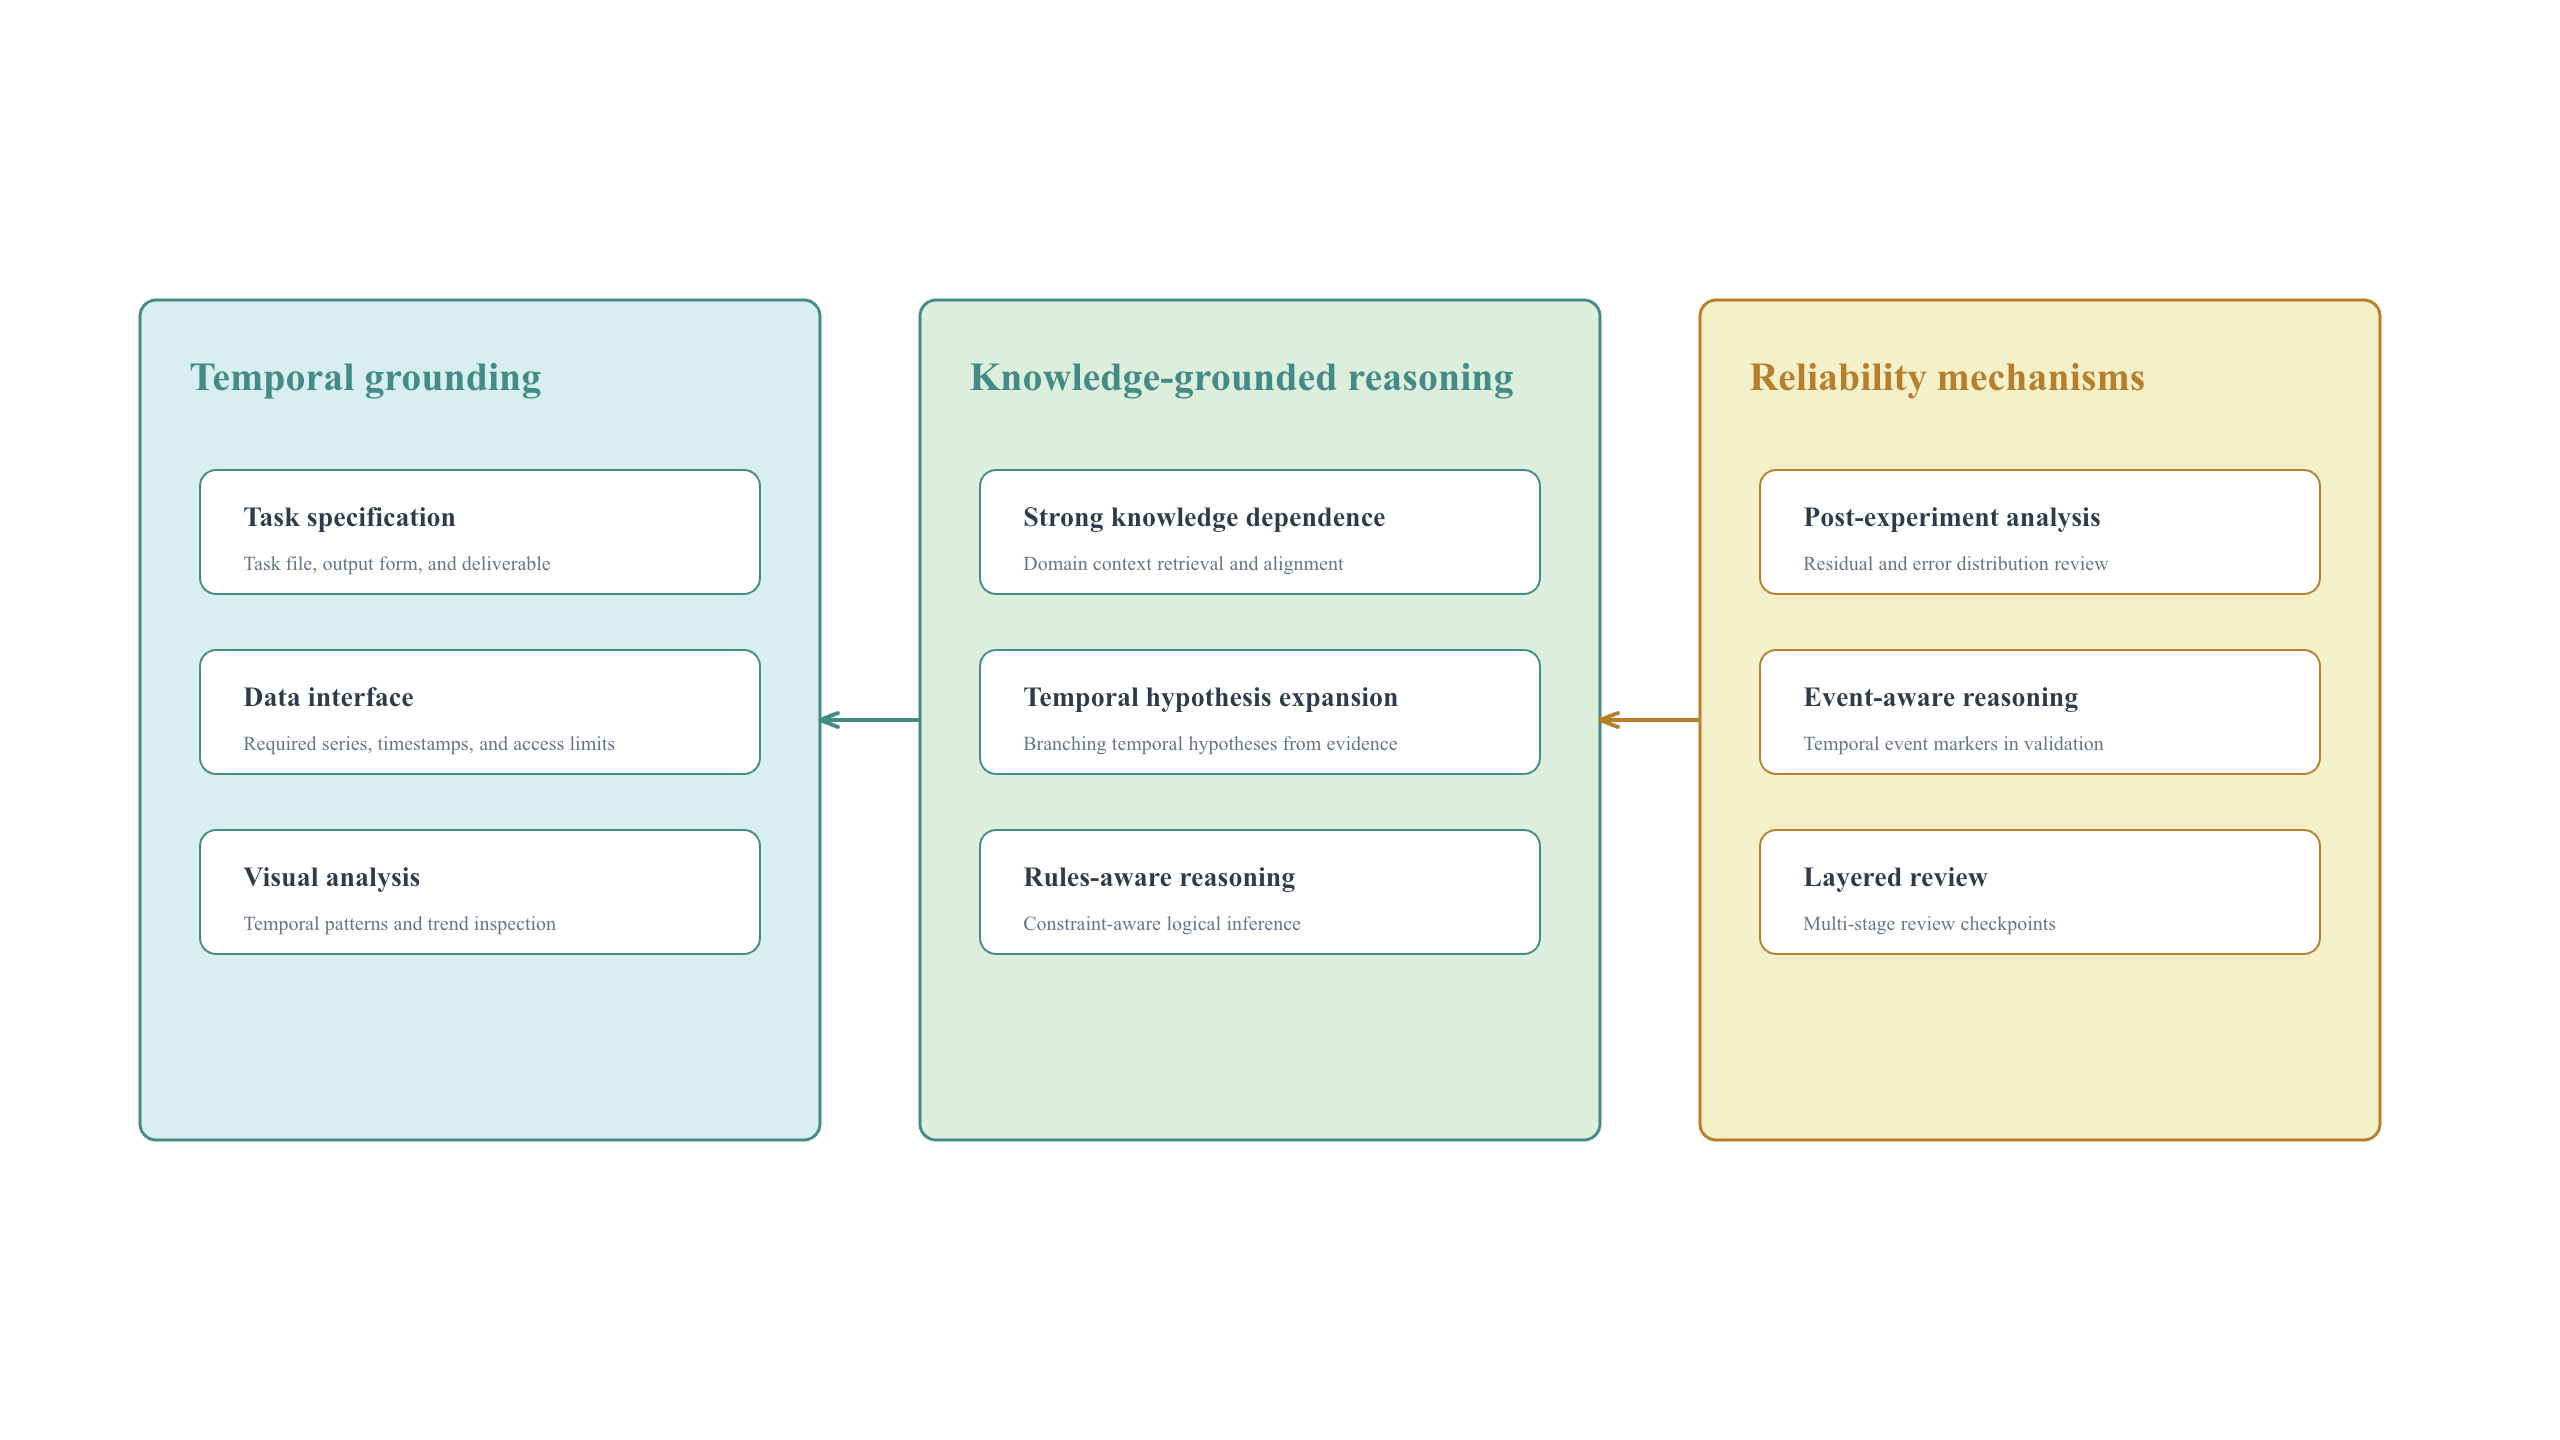
\includegraphics[width=0.90\linewidth]{artifacts/active/Figure_support_aion.png}
\caption{AION's three coupled time-series harness principles, adapted and redrawn from Fig.~2 of \citet{aion2026}. Temporal grounding, knowledge-grounded reasoning, and reliability mechanisms show why GTS is a temporal contract layered on top of a general runtime.}
\label{fig:aion-principles}
\end{figure}

The following subsections retain the seven dimensions in Table~\ref{tab:component-vocab}. Each identifies the temporal content added to that mechanism and the point where a task-specific objective enters.

\subsection{Interface and Interaction}

The temporal interface assigns meaning to observations and operations: timestamps, sampling frequency, observation windows, channels, and allowed history. AION \citep{aion2026}, Section~3.3.1, first resolves the observation unit, requested window, time granularity, and leakage boundary. Its data interface connects those requirements to heterogeneous files and partially observed tables. The resulting interface can support a forecast table, a structured answer, or a report because the observation semantics are specified separately from the output metric.

TIMECLAW \citep{timeclaw2026harness} provides a complementary implementation. Full-precision series reside in a task-local workspace; the LLM specifies an operation and its parameters through a typed executable interface. The returned observation is compact, while the underlying numerical object remains in the runtime. This boundary preserves temporal data without requiring the model to reconstruct an entire series from a dialogue history.

\subsection{Memory and Context}

Temporal retrieval depends on both the analytical question and the signal being analyzed. TIMECLAW \citep{timeclaw2026harness}, Section~3.4, stores a task, signal and text retrieval keys, its successful trajectory, and a transferable rationale. Its memory record is
\begin{equation}
  m=(\mathcal{T},\phi,\psi,\zeta,\rho),
  \label{eq:timeclaw-memory}
\end{equation}
where $\phi$ and $\psi$ represent signal and text keys, $\zeta$ is the analytical trace, and $\rho$ summarizes the contextual cue and rule behind the solution. The two retrieval modalities address different similarities: two requests may have similar wording but different temporal structure, or similar signal shapes but different contextual causes.

This mechanism explains what temporal memory adds to the general memory in Section~\ref{sec:general-harness}. The runtime still stores and retrieves records, but relevance now depends on numerical structure as well as language. When such records guide a historical decision, their admissibility also depends on when the information became available. A memory implementation and its evaluation should therefore expose the signal representation, retrieval keys, and access policy used by the analysis.

\subsection{Tools and Execution}

TIMECLAW \citep{timeclaw2026harness}, Section~3.2, runs temporal operations inside the workspace and returns structured observations. Slicing, aggregation, decomposition, smoothing, and numerical inspection operate on the resident series. An auditable trajectory links the analytical intent and tool observation to the final answer. These operations supply common temporal capabilities that different task procedures can call.

TimeSeriesScientist's Curator \citep{timeseriesscientist2025}, Section~3.2, illustrates a concrete preprocessing module. It diagnoses statistics, missingness, and outliers before choosing a transformation:
\begin{equation}
  Q=A_f(D)=(S,M,O,\pi),\qquad
  \widetilde{D}=\phi_{\pi}(D),
  \label{eq:tsci-curator}
\end{equation}
Here $S$ contains summary statistics and trend information, $M$ records missing values, $O$ records outliers, and $\pi$ specifies the recommended treatment. The processed series then supports visualization, decomposition, and autocorrelation analysis. This operation can be described independently of the subsequent forecast model selection: it produces a characterized and processed series, while the task module determines which model and output are appropriate.

\subsection{Control, Verification, and Feedback}

Temporal verification checks whether an output is consistent with the temporal data and access rules. AION \citep{aion2026}, Section~3.1, defines a validator that returns validity checks separately from scored metrics. Its examples include timestamp alignment, leakage boundaries, and format compliance. Section~3.3.1 connects these checks to the observation window, output granularity, and allowed history. A candidate can therefore be returned for revision before its numerical score is compared with other candidates.

The shared operation is checking temporal admissibility; a particular loss or utility belongs to the task. For example, detecting a future observation in a retrieval is different from measuring forecast MAE, and detecting a misaligned timestamp is different from scoring an anomaly interval. This separation lets the same chronology and alignment checks accompany several task-specific evaluators. AION evaluates its architecture in a Store Sales case study; that study supplies concrete implementation evidence for the reported setting.

\subsection{Planning and Workflow}

A temporal plan must preserve the meaning of its intermediate artifacts. AION \citep{aion2026} resolves the task specification and data interface before accepting a candidate output. If the observation window, output mode, or granularity fails the constraints, the candidate returns for revision. These checkpoints carry the temporal contract through a workflow whose general execution and review protocols were described in Section~\ref{sec:general-harness}.

The reusable checkpoint asks whether the data and artifact match the declared temporal scope. Rolling-origin selection, forecast-horizon optimization, and anomaly escalation add particular task procedures. They are developed in Section~\ref{sec:task-specific-harness}, where their objectives and feedback can be compared directly. A task-changing workflow can retain the temporal checkpoints while replacing the operations between them.

\subsection{Optimization and Evolution}

Temporal capability evolution concerns the content of the procedure being learned from experience. TIMECLAW \citep{timeclaw2026harness} extracts recurring analytical subprocedures into tools that operate on the temporal workspace. Their invocation description and implementation must preserve the input series and the meaning of the returned observation. The general promotion mechanism tests and registers candidates; the candidate's temporal computation determines its GTS or TSK scope.

This distinction gives a practical criterion for reuse. A learned series transformation that returns the same kind of temporal object across tasks can extend the shared toolkit. A routine that selects a forecast using forecast error retains a forecasting contract. The classification therefore follows the individual procedure and its input--output semantics, rather than treating all tools produced by one evolving agent as equally general.

\subsection{Coordination and Scaling}

When several agents analyze temporal evidence, their handoff must preserve the observation window and the identity of the data being discussed. AION \citep{aion2026} combines a shared workspace and temporal constraints with review and communication protocols. This provides a way for an analyst and reviewer to refer to the same candidate artifact and the conditions under which it was produced.

The coordination protocol remains a General Harness mechanism. A separate temporal contribution is present when the handoff itself carries and checks temporal meaning, such as the window or aligned observations. In system construction, this means that different roles should receive the temporal scope with the artifact they inspect. The same seven mechanism dimensions thus describe both the runtime and its temporal specialization; the subsequent task sections instantiate them under concrete outputs and objectives.

\section{Task-Specific Time-Series Harness}
\label{sec:task-specific-harness}

Task-specific Harness modules instantiate the General Time-Series Harness under a concrete output contract. Four task families organize this section, each analyzed through interface, memory, tools, control and verification, planning, optimization, and coordination.

The task contract determines the final object being optimized. For forecasting, a typical contract is
\begin{equation}
  \widehat{y}_{\tau+1:\tau+H}=f_\theta\!\left(y_{\leq\tau},x_{\leq\tau}\right),
  \label{eq:forecast-contract}
\end{equation}
where $H$ is the declared horizon and the inputs are restricted by the availability set in Eq.~\ref{eq:temporal-availability}.

\noindent\textbf{Purpose of the task-family figure.} The four branches show how one shared Harness vocabulary becomes four different output contracts. Read each branch from temporal input to validation: forecasting emphasizes horizon and backtesting, augmentation emphasizes fidelity and utility, anomaly diagnosis emphasizes localization and evidence, and decision support emphasizes utility, risk, cost, and review authority. This figure explains why task categories are an instantiation layer rather than a competing top-level taxonomy.

\begin{figure}[htbp]
\centering
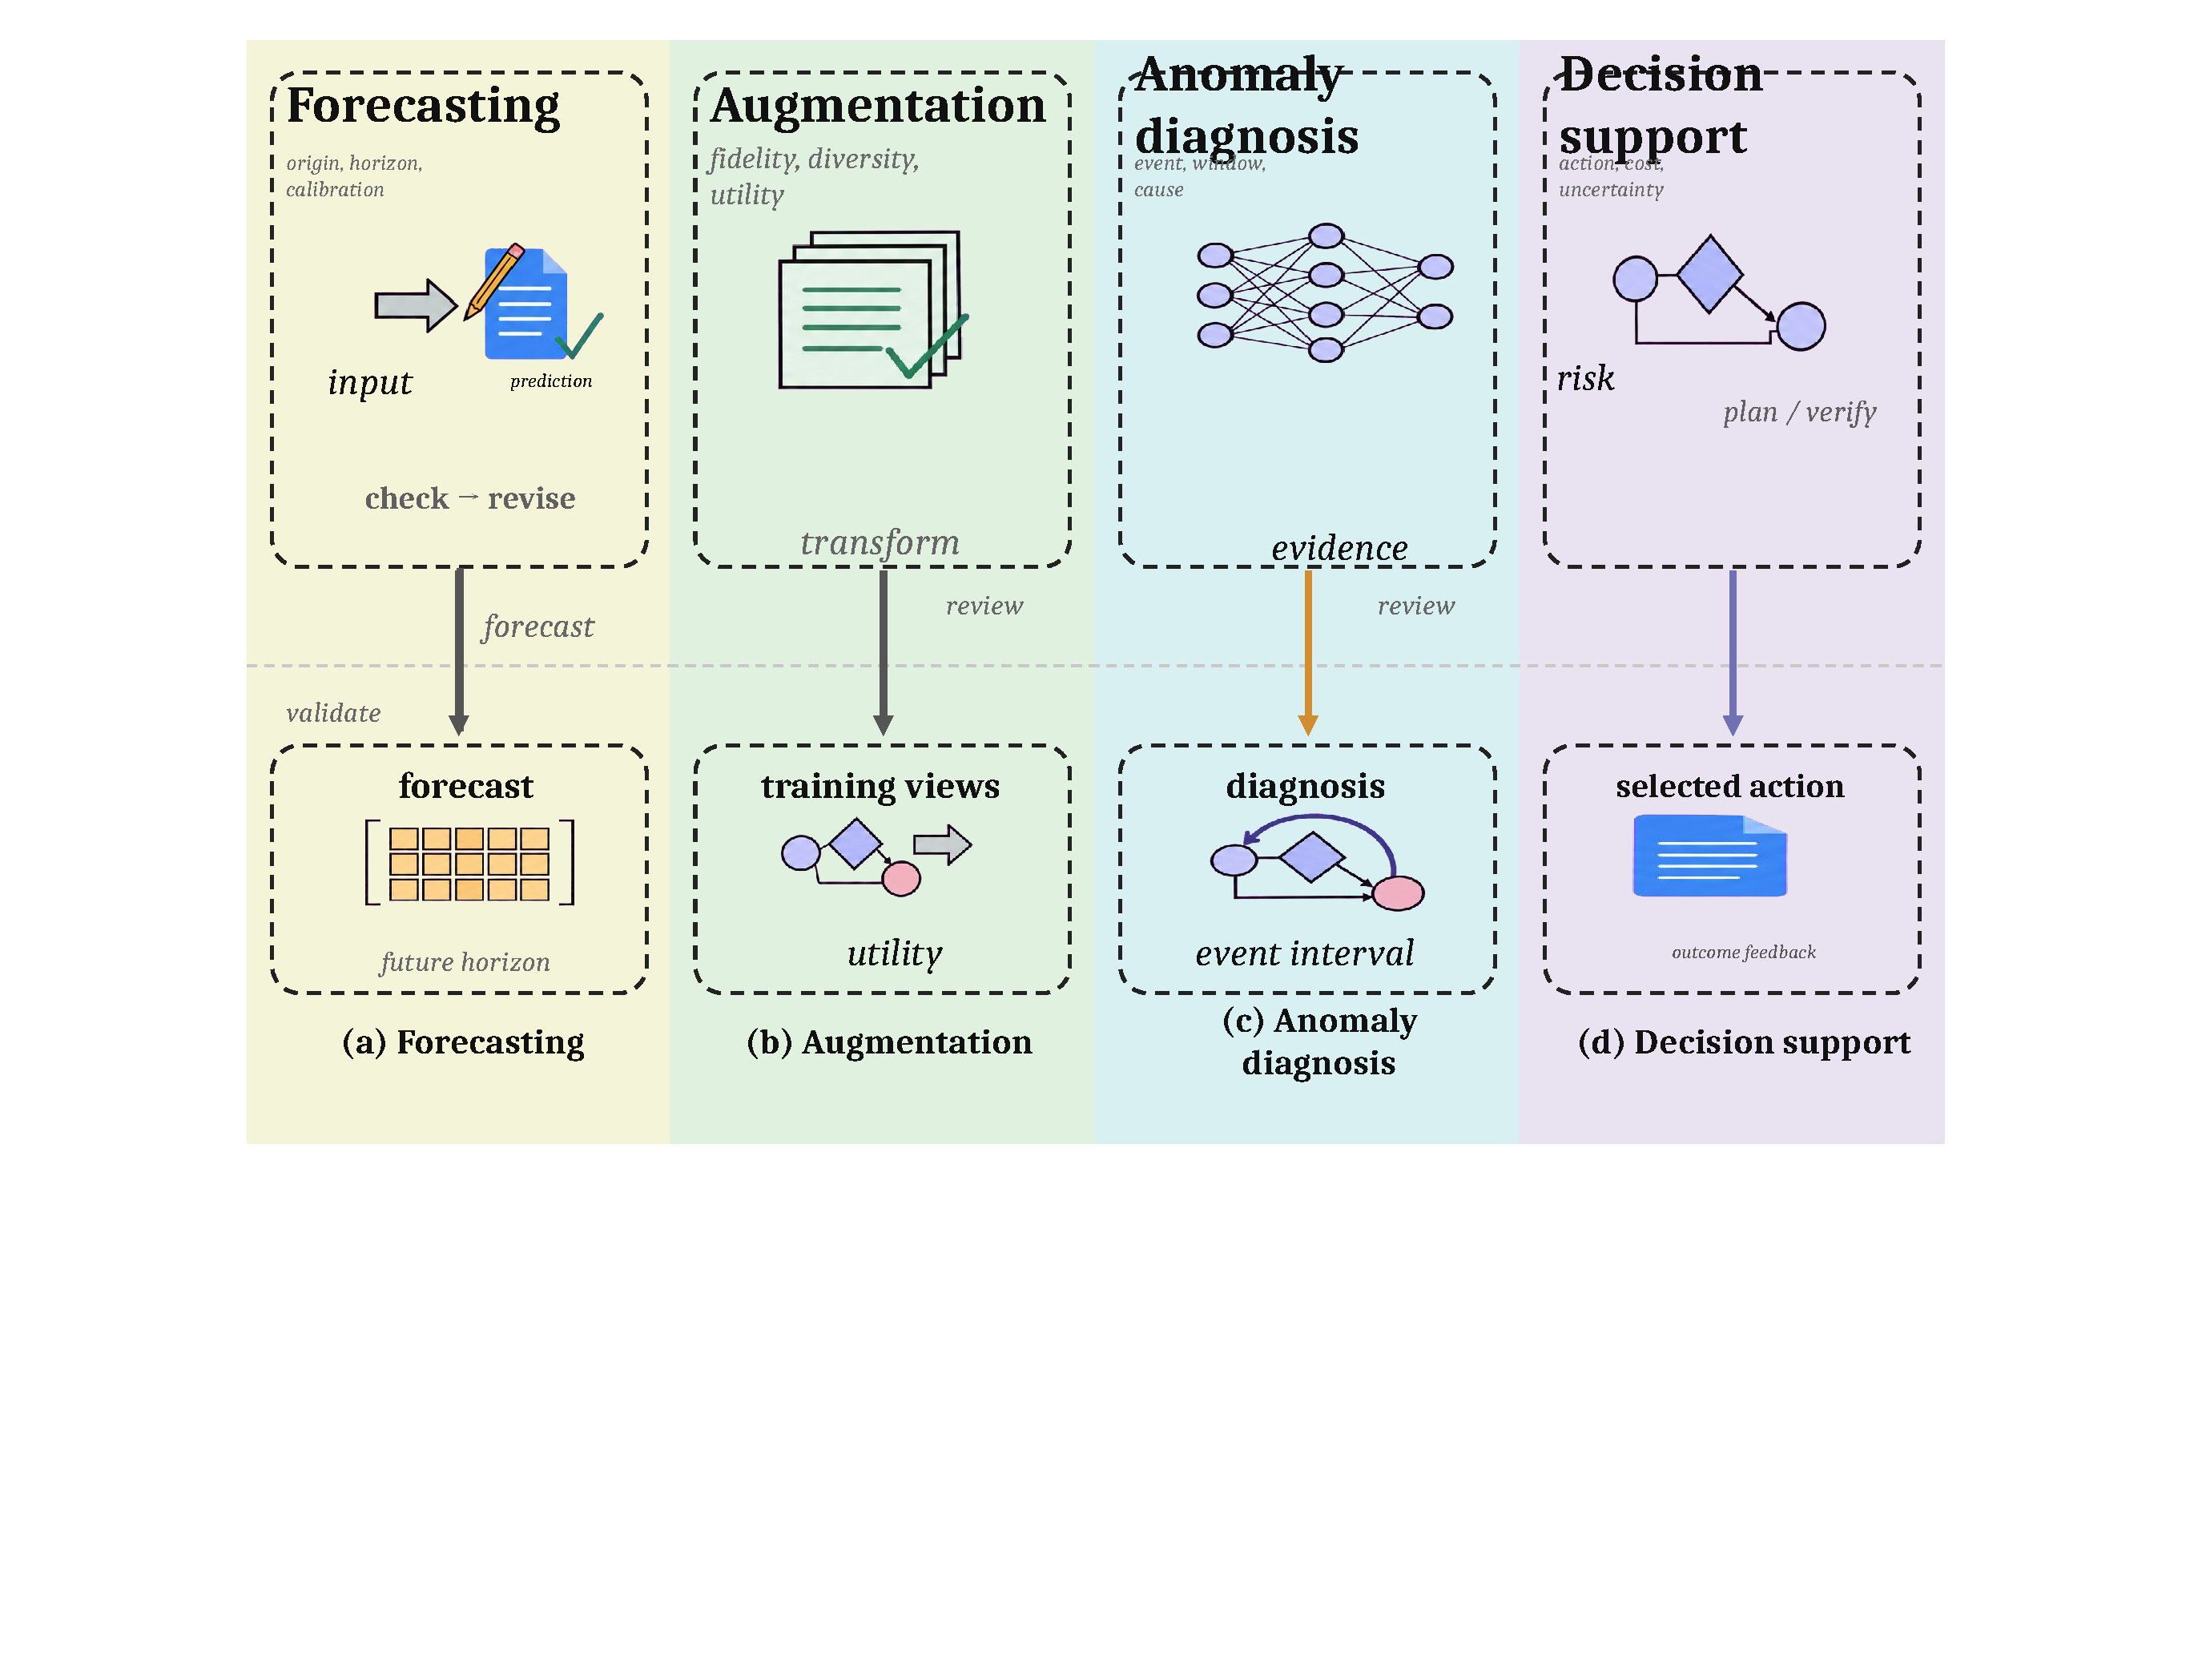
\includegraphics[width=0.98\linewidth]{artifacts/active/Figure6_task_contracts_rsi_adapted.pdf}
\caption{The four task families and their task-specific Harness contracts. Each family instantiates the same seven-module lens under a different temporal output contract. The editable source is adapted from the RSI-style survey template and rewritten for this survey.}
\label{fig:task-specific-harness}
\end{figure}

\subsection{Forecasting and Prediction}

Forecasting fixes an origin, target, horizon, and evaluation rule. The agent must choose how to build a forecast, which contextual evidence to use, and when to revise it. Numerical prediction produces future values or a predictive distribution; event prediction produces classes or probabilities for future outcomes. These contracts lead to different model interfaces and scoring rules.

TimeSeriesScientist \citep{timeseriesscientist2025} develops a numerical forecasting workflow in which the Curator's diagnostics guide the Planner's model search. For each candidate forecaster, the Planner tunes its configuration using validation MAPE:
\begin{equation}
  \theta_i^{\star}=\arg\min_{\theta_i\in\mathcal{C}_i}
  \operatorname{MAPE}_{\mathrm{val}}\!\left(m_i(\theta_i)\right),\qquad
  \operatorname{MAPE}_{\mathrm{val}}(m_i(\theta_i))=
  \frac{100\%}{|\widetilde{D}_{\mathrm{val}}|}
  \sum_{t\in\widetilde{D}_{\mathrm{val}}}
  \left|\frac{x_t-\widehat{x}^{(i,\theta_i)}_t}{x_t}\right|.
  \label{eq:tsci-planner}
\end{equation}
The selected configurations are ranked, and the Forecaster reasons over the top candidates and their validation results to choose a single model or ensemble. This links the temporal diagnostics in Section~\ref{sec:general-ts-harness} to a task-specific selection criterion. TimeCopilot \citep{timecopilot2025} likewise makes forecasting models callable components; the model library supplies numerical capabilities while the agent organizes their use.

FLAIRR-TS \citep{flairr2025}, Algorithm~1, refines the forecasting prompt through retrieved historical segments and observed forecast errors:
\begin{equation}
\begin{aligned}
  S_{\mathrm{retr}}^{(k)}&=\operatorname{RetrieveSegments}(X_{\mathrm{HistDB}},X_{\mathrm{Ctx}},M),\\
  C_{\mathrm{aug}}^{(k)}&=\operatorname{AugmentContext}(X_{\mathrm{Ctx}},S_{\mathrm{retr}}^{(k)}),\\
  \widehat{X}^{(k)}&=F_{\mathrm{LLM}}(P_{\mathrm{curr}}^{(k)},C_{\mathrm{aug}}^{(k)},H),\\
  \operatorname{mae}^{(k)}&=\operatorname{MAE}(\widehat{X}^{(k)},X_{t:t+H}),\\
  (P_{\mathrm{next}}^{(k)},d^{(k)})&=R_{\mathrm{LLM}}\!\left(\{(P^{(i)},\operatorname{mae}^{(i)})\}_{i<k},P_{\mathrm{curr}}^{(k)},\tau_{\mathrm{stop}}\right).
\end{aligned}
\label{eq:flairr-loop}
\end{equation}
The refiner receives the history of prompts and errors, proposes an update, and may stop the loop. At the iteration limit the procedure returns the prompt with the lowest observed MAE. The algorithm explicitly takes recent ground truth as an input, so the error-driven update runs on resolved forecast windows. Its feedback schedule is part of the forecasting procedure.

CastFSR \citep{castfsr2026} separates fast numerical forecasting, slower contextual deliberation, and reflective evaluation. The initial prediction supplies a numerical prior; retrieved context then supports a candidate revision. Its state and action families make that division explicit:
\begin{equation}
  s_k=\Phi(I,M_k,\widehat{Y}^{\mathrm{prior}}_k,C_k),\qquad
  a_k\sim\pi_{\theta}(\cdot\mid s_k),\quad a_k\in\mathcal{A}_{\mathrm{fast}}\cup\mathcal{A}_{\mathrm{slow}}\cup\mathcal{A}_{\mathrm{reflect}}\cup\mathcal{A}_{\mathrm{final}}.
  \label{eq:castfsr-state-action}
\end{equation}
\begin{equation}
\begin{aligned}
  C_k&=T_{\mathrm{ctx}}(D_{\mathrm{task}},D_{\mathrm{domain}},X_{1:L},H_{\mathrm{ctx}},\widehat{Y}^{\mathrm{prior}}_k,M_k;W_k),\\
  \widehat{Y}^{\mathrm{cand}}_k&=G_{\theta}(\widehat{Y}^{\mathrm{prior}}_k,C_k,M_k),\\
  E_k&=E_{\theta}(\widehat{Y}^{\mathrm{cand}}_k,\widehat{Y}^{\mathrm{prior}}_k,C_k,M_k),\qquad
  \widehat{Y}_{1:H}=F_{\theta}(\widehat{Y}^{\mathrm{cand}}_k,E_k,M_k).
\end{aligned}
\label{eq:castfsr-revision}
\end{equation}
The method's distinction lies in how context changes a forecast prior and how reflection assesses the candidate. It belongs here because the state includes a forecast, the actions revise that forecast, and the final output is a numerical horizon. Last-Mile Forecasting \citep{lastmile2026} and CastFlow \citep{castflow2026} provide related settings for contextual revision, while HydroAgent \citep{hydroagent2026} connects predictions to hydrological simulation and warnings.

SCENARIODIFF \citep{scenariodiff2026} uses a Historical Context Agent, a Scenario Agent, and an Anchor Guidance Agent to translate documents into historical summaries, a future scenario, and sparse anchor constraints. A diffusion forecaster generates the future trajectory conditioned on this information:
\begin{equation}
  \mathcal{L}(\theta)=\mathbb{E}_{x^{(0)},t,\epsilon}
  \left\|x^{(0)}-x_{\theta}\!\left(x^{(t)},t,c\right)\right\|_2^2,
  \qquad
  x^{(t)}=\sqrt{\bar\alpha_t}x^{(0)}+\sqrt{1-\bar\alpha_t}\,\epsilon,
  \label{eq:scenariodiff-denoising}
\end{equation}
Here $x^{(0)}$ is the future target horizon and $c$ contains the historical and scenario context. Anchor Blended Sampling then uses the anchors to refine the sampled trajectory. The generation step therefore implements probabilistic forecasting. It differs from the training-series generation below in both its output and its evaluation target.

Event forecasting uses a different output space. TimeCAP \citep{timecap2025} connects contextualization and prediction through two agents:
\begin{equation}
  s_x=A_C(x)=M_{\theta}\!\left(p_C(x)\right),\qquad
  \widehat{y}_{\mathrm{LLM}}=A_P(s_x)=M_{\theta}\!\left(p_P(s_x)\right).
  \label{eq:timecap-dual-agent}
\end{equation}
The contextualizer converts a series into a textual summary, and the predictor uses that summary to estimate the outcome. AIA Forecaster \citep{aiaforecaster2025} combines search, supervisor aggregation, and calibration for judgmental event forecasts; AUDITFORECAST \citep{auditforecast2026} anchors predictions in a quantitative baseline and updates them in odds space. These methods require probability and outcome evaluation alongside evidence access and trace inspection. Their comparison is most informative when the target event, resolution time, and available evidence are fixed.

\subsection{Data Augmentation and Synthesis}

Augmentation and synthesis create examples for learning or analysis. The output may be a transformed positive view, an additional training series, or a temporal instruction dialogue. Its evaluation depends on that use: preserving a useful representation, training an accurate downstream model, and teaching a language model require different checks.

MERIT \citep{merit2025} targets unsupervised time-series representation learning. A retrieval agent selects relevant series from a candidate set; an augmentation agent uses those examples to choose transformations; and a review agent assesses the resulting positive views and controls whether generation continues. The retrieved and augmented views then support contrastive learning. The review acts on the generated examples during construction, while downstream experiments evaluate the learned representation. Figure~\ref{fig:merit-augmentation} shows this separation between retrieval, transformation, and review.

MetaCaster \citep{metacaster2026} generates training series from a small support set and domain context, then trains lightweight forecasters on the generated data. Its Harness Proposer changes the generator's prompts and skills to improve the downstream forecasting result. The optimization objective compares forecasters trained on authentic and generated data:
\begin{equation}
  \theta^{\star}=\arg\min_{\theta}\;\mathbb{E}_{m,l}\,\delta\!\left(\omega(f_l^m),\omega(\bar f_l^m)\right),\qquad
  \bar D^m=\operatorname{MGAgent}(D_{\mathrm{sup}}^m,C^m),
  \label{eq:metacaster-objective}
\end{equation}
\begin{equation}
  \delta\!\left(\omega(f_l^m),\omega(\bar f_l^m)\right)=
  \max\!\left\{\frac{\omega(\bar f_l^m)-\omega(f_l^m)}{\omega(f_l^m)},0\right\}
  \label{eq:metacaster-hinge}
\end{equation}
Here $\omega$ measures forecasting error and the hinge-style discrepancy penalizes a generated-data forecaster when it performs worse. Generation and harness optimization are coupled to the forecasting objective; the job scheduler and recovery mechanism remain separately reusable General Harness components. This provides a concrete example of one paper contributing distinct modules at different layers.

ChatAD \citep{chatad2026} constructs temporal instruction dialogues through TSEvol. A Consultant and Client generate reasoning exchanges, while an Intern and Supervisor support iterative assessment and refinement. These agents operate during training-data construction. The resulting supervision is then used to adapt the language model, as described in Section~3. BRIDGE \citep{bridge2025} provides a complementary language-conditioned temporal generation setting. Comparing these methods requires identifying the generated object and the learner or analysis it is intended to support.

\noindent\textbf{Why the augmentation example matters.} The MERIT loop shows a concrete task-specific contract: generation is followed by retrieval, review, and downstream-utility checks. Read the loop as evidence that synthetic data are not validated by resemblance alone; fidelity and usefulness are jointly evaluated. The diagram is adapted from MERIT~\citep{merit2025}.

\begin{figure}[htbp]
\centering
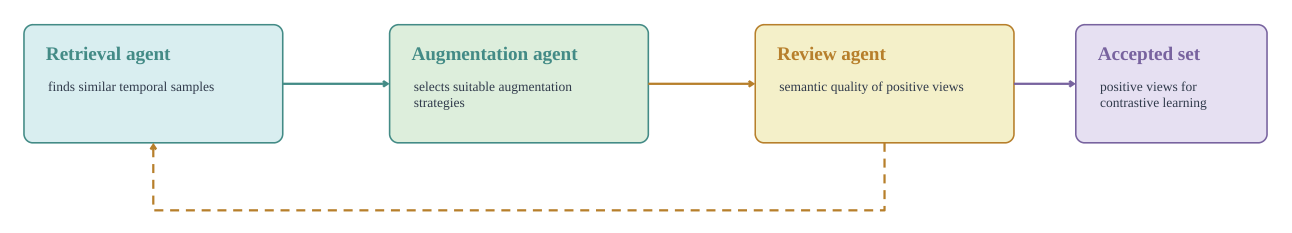
\includegraphics[width=0.94\linewidth]{artifacts/active/Figure_support_merit.png}
\caption{MERIT's retrieval--augmentation--review loop, adapted and redrawn from Fig.~2 of \citet{merit2025}. The generator is coupled to a task-specific review agent, making fidelity and downstream utility part of the augmentation contract.}
\label{fig:merit-augmentation}
\end{figure}

\subsection{Anomaly Detection and Diagnosis}

Anomaly agents localize events, propose or verify rules, retrieve incident evidence, diagnose causes, and support remediation. AnomaMind \citep{anomamind2026} separates coarse evidence acquisition, adaptive evidence construction, detection, and iterative refinement. ChatAD \citep{chatad2026} trains an anomaly-reasoning model using evolved instruction data and subsequent preference optimization, while SAGE-AD \citep{sagead2026} and LEMAD \citep{ji2025lemad} connect detection to diagnosis and service context. Large-model-based smart agents \citep{wang2026large} use temporal evidence to interpret power-system anomalies. The TSK contract fixes monitoring windows, thresholds, root-cause labels, false-alarm budgets, alert policies, and deployment gates. AnomaMind makes the sequential structure explicit: at step $k$, the agent maintains a state $s_k$, selects an action $a_k$, and receives numerical or knowledge evidence $o_k$ from its toolkit. Its toolkit is written as $B=\{K,N\}$, where $K$ denotes knowledge memory and $N$ numerical diagnostics. The paper's workflow update and detector are
\begin{equation}
  s_{k+1}=E\!\left(s_k,a_k,o_k,\widehat{Y}^{(k)}\right),\qquad
  \widehat{y}_j=D_{\theta}\!\left(s_j,Z_{1:k},C_{1:k}\right),\quad \widehat{y}_j\in\{0,1\},
  \label{eq:anomamind-decision}
\end{equation}
and its rule-based feedback combines parse validity, interval F1, and a false-positive penalty,
\begin{equation}
  r_k=\lambda_p r_k^{\mathrm{parse}}+\lambda_f r_k^{F1}-\lambda_{fp}r_k^{FP},\qquad
  \max_{\theta}\;\mathbb{E}_{\widehat{Y}^{(k)}\sim\pi_{\theta}(\cdot\mid s_k)}\left[\sum_{k=1}^{K}r_k\right].
  \label{eq:anomamind-reward}
\end{equation}
This is the method-level distinction: the LLM gathers evidence and reflects, while the detection policy receives task-specific learning signals \citep{anomamind2026}. Anomaly detection therefore proceeds through evidence-seeking decisions, tool responses, and state updates rather than a single fixed score.

\noindent\textbf{Why the anomaly example matters.} AnomaMind makes the anomaly contract visible as a coarse-to-fine workflow: acquire evidence, detect a suspicious interval, diagnose a cause, and refine the conclusion. The figure maps each stage to a TSK module and shows why detection accuracy alone does not establish diagnostic quality. It is adapted from AnomaMind~\citep{anomamind2026}.

\begin{figure}[htbp]
\centering
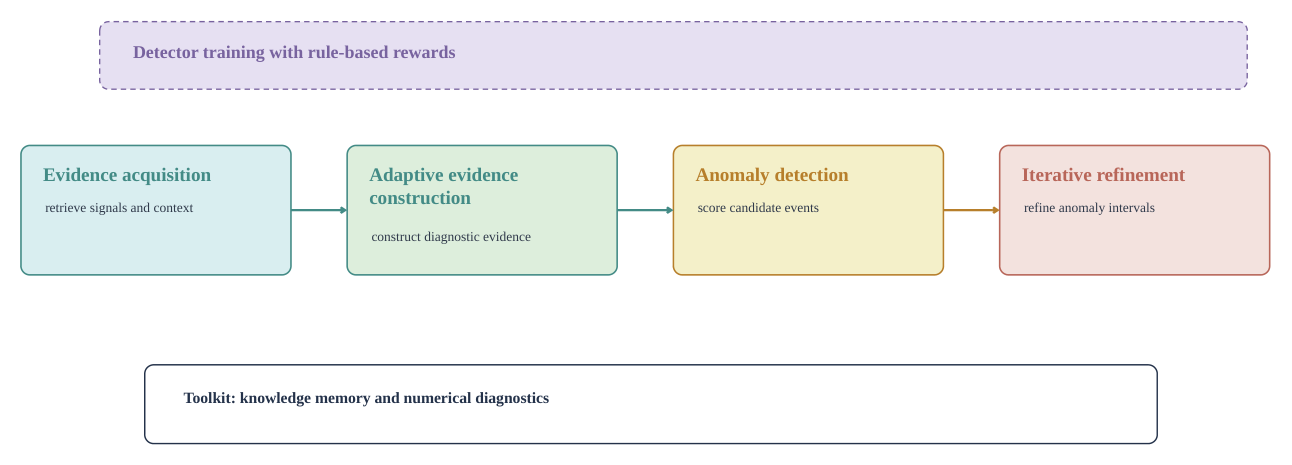
\includegraphics[width=0.96\linewidth]{artifacts/active/Figure_support_anomamind.png}
\caption{AnomaMind's coarse-to-fine anomaly-diagnosis workflow, adapted and redrawn from Fig.~1 of \citet{anomamind2026}. The example separates evidence acquisition, detection, diagnosis, and iterative refinement, which are distinct TSK modules under the anomaly contract.}
\label{fig:anomamind-workflow}
\end{figure}

\subsection{Decision Support}

Decision-support agents connect forecasts or diagnoses to actions under costs, constraints, uncertainty, and review requirements. Prediction-market theory makes the forecast-to-action link explicit: a forecast becomes useful through a market-dependent scoring and betting rule, which is a complementary decision contract for agent evaluation \citep{prophets2026}. FinCon \citep{fincon2024} coordinates analyst evidence before portfolio decisions, TradingAgents \citep{tradingagents2024} turns market and news analysis into risk-aware trading actions, and CoLLMLight \citep{collmllight2026} uses simulation feedback for network-wide signal control. ClimateAgent \citep{climateagent2025} connects climate analysis to operational workflows, while Smart Energy Agent \citep{smartenergyagent2026} converts appliance-level anomalies into maintenance recommendations. FinCon states the decision objective directly as cumulative profit and loss under prompt-controlled analyst and manager policies,
\begin{equation}
  \max_{\theta}\;\mathbb{E}\!\left[\sum_{t\in\mathcal{T}}\alpha^t R_t^{\Pi_{\theta}}\right],
  \qquad R_t^{\Pi_{\theta}}=R(O_t,B_t,A_t),
  \label{eq:fincon-objective}
\end{equation}
and its portfolio manager solves a mean--variance allocation subject to the buy/sell/hold direction selected by the agents,
\begin{equation}
  \max_{w}\;\langle w,\mu\rangle-\langle w,\Sigma w\rangle,\qquad
  w_n\in\begin{cases}[0,1],&\text{buy},\\\left[-1,0\right],&\text{sell},\\\{0\},&\text{hold},\end{cases}
  \quad n=1,\ldots,N.
  \label{eq:fincon-portfolio}
\end{equation}
These equations show how the multi-agent Harness turns temporal evidence into a task-specific action and risk contract \citep{fincon2024}. The TSK interface represents the current state, available actions, timing, and authority; control checks risk limits and counterfactual consequences; and human review records whether the recommendation was accepted, revised, or escalated.

Decision support extends prediction through an action utility:
\begin{equation}
  a_{\tau}^{\star}=\arg\max_{a\in\mathcal{A}}\mathbb{E}\!\left[U(a,Y_{\tau+1})\mid\mathcal{I}_{\tau}\right],
  \label{eq:decision-contract}
\end{equation}
where the utility, action set, uncertainty, and review authority are part of the task contract. This makes the transition from forecasting to decision support explicit.

The complete corpus is multi-label across components: a work may contribute to several Harness dimensions and task families, with each component assigned to its deepest applicable Harness layer. The maintained ledger records both the inclusive evidence fields and the exclusive plotting labels, alongside the independent LLM-side contribution.
\section{Infrastructure and Benchmarks for Time-Series Agents}
\label{sec:evaluation}

A Time-Series Agent requires evaluation at three levels: General Harness process, time-series contract, and task outcome. Existing resources cover fragments of this contract; the benchmark gap is the absence of a widely adopted cross-task suite that evaluates them together. AION makes the missing task contract explicit by representing a next-generation time-series task as
\begin{equation}
  \mathcal{T}=(\phi,\mathcal{W},\mathcal{V}),\qquad
  \phi=(\mathcal{T}_{\mathrm{access}},\Sigma,\mathcal{O},\mathcal{C},\mathcal{A}),\qquad
  (g,s)=\mathcal{V}(o),
  \label{eq:aion-task-contract}
\end{equation}
where the task file specifies access, prior knowledge, output form, constraints, and metrics, while the validation interface returns validity checks $g$ and scores $s$ for a candidate output $o$ \citep{aion2026}. This formalization is why a benchmark must expose the workspace and validation interface rather than only a dataset and one score.

\subsection{Evaluation contract}

Evaluation should report tool-call validity, trace faithfulness, memory and artifact provenance, temporal availability rules, numerical fidelity, temporal operations, evidence grounding, task metrics, cost, failures, and revision behavior. A forecast or QA score is one task result within a complete Agent evaluation.

The unit of evaluation is an episode. An episode records the task specification, as-of boundary, visible context, tool calls, intermediate artifacts, validator decisions, revision steps, final output, and resource use. This record attributes errors to prediction, tool selection, leakage, temporal operations, or revision after feedback.

We represent an episode as
\begin{equation}
  e=\bigl(\mathcal{C}_{\mathrm{task}},\tau,\mathcal{I}_{\tau},\omega_{1:K},\mathcal{V}_{1:K},r,\operatorname{Cost}(e)\bigr),
  \label{eq:episode-record}
\end{equation}
which keeps the task contract, information boundary, execution trace, verification decisions, final result, and resource use in one auditable record. A benchmark reports a vector of process validity, temporal-contract validity, task outcome, and resource behavior:
\begin{equation}
  \mathcal{E}(e)=\bigl(E_{\mathrm{GH}},E_{\mathrm{GTS}},E_{\mathrm{TSK}},E_{\mathrm{resource}}\bigr),
  \label{eq:evaluation-vector}
\end{equation}
where the four coordinates measure process validity, temporal-contract validity, task outcome, and cost or failure behavior. The vector follows the construction hierarchy and makes clear which layer a benchmark actually tests.

The same protocol should support controlled perturbations: hide or reveal contextual evidence, shift the forecast origin, inject missingness, change the frequency, or replace a tool with a failing implementation. These interventions expose whether a system relies on the intended temporal evidence and whether its General Harness can recover from operational failures.

\noindent\textbf{How to read the evaluation stack.} The stack aligns evaluation with the construction hierarchy: process validity at the runtime layer, temporal-contract validity at the GTS layer, task outcomes at the TSK layer, and reproducibility across the full episode. Its purpose is to prevent a single forecast or QA score from standing in for tool correctness, chronology, evidence quality, and revision behavior. The episode record is linked to the benchmark discussion that follows.

\begin{figure}[htbp]
\centering
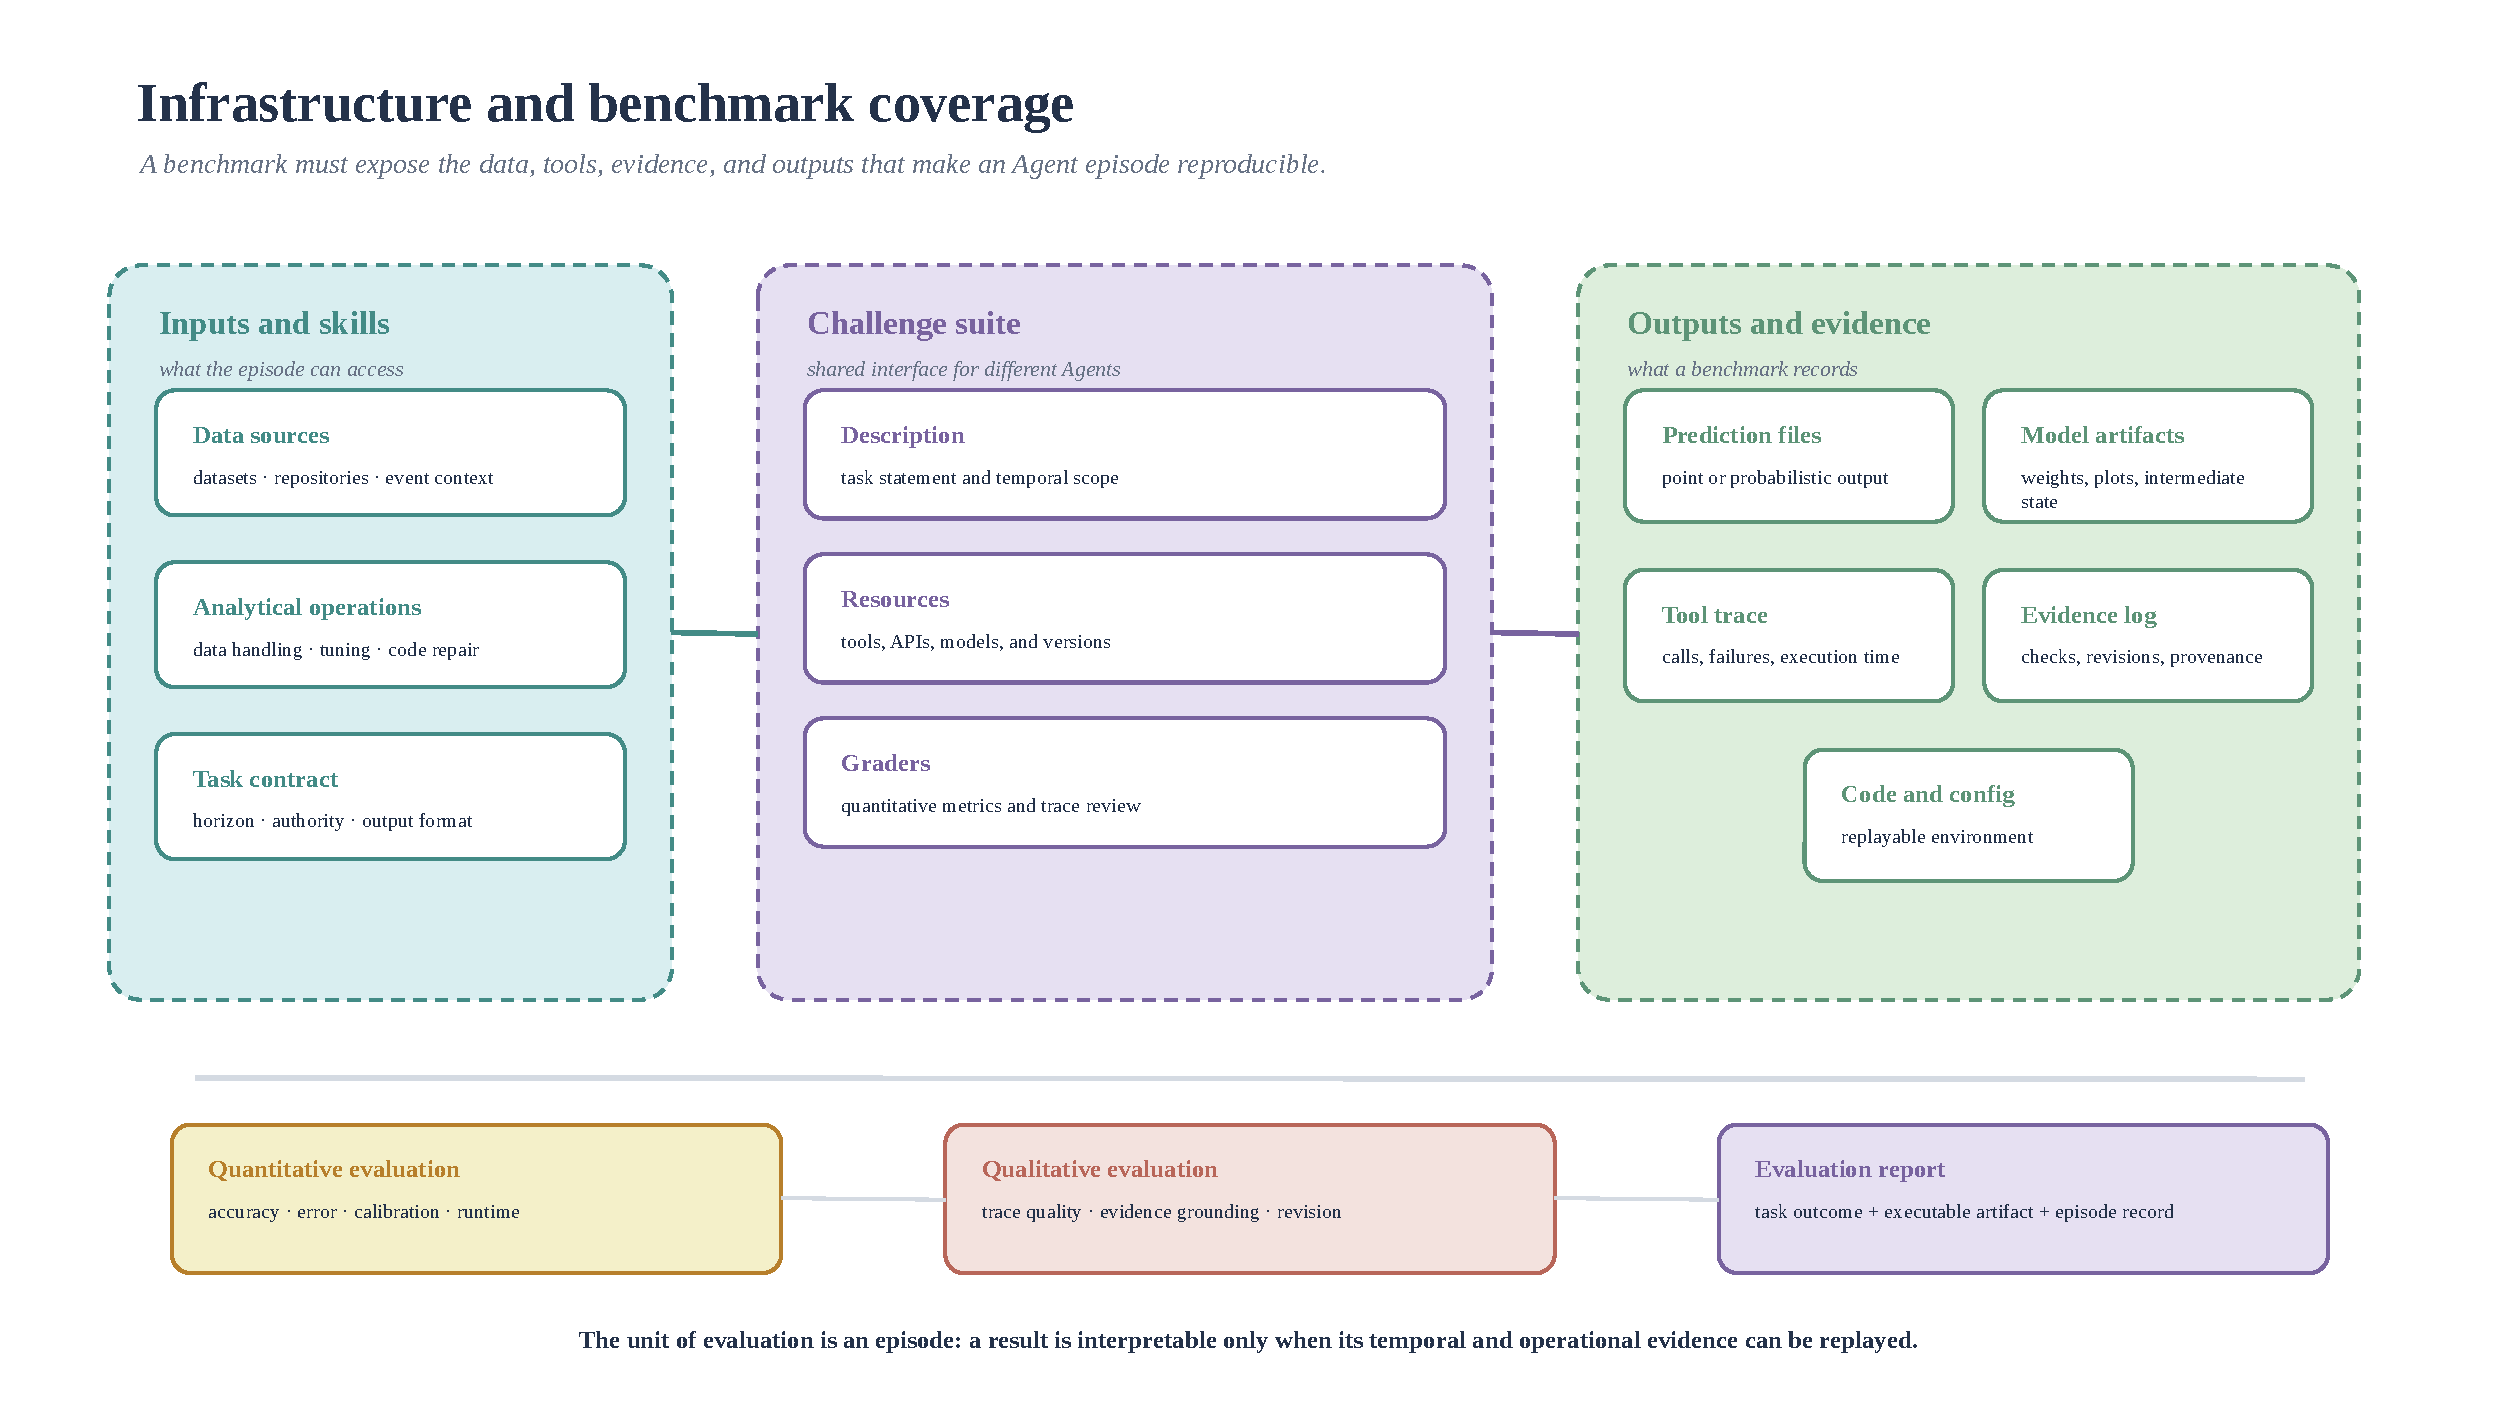
\includegraphics[width=0.98\linewidth]{artifacts/active/Figure7_infrastructure_native.pdf}
\caption{Infrastructure and benchmark coverage. The evaluation layers mirror the construction hierarchy, while the episode record preserves temporal availability, execution, evidence, revision, and reproducibility.}
\label{fig:evaluation-stack}
\end{figure}

\subsection{Existing benchmark landscape}

\begin{figure}[htbp]
\centering
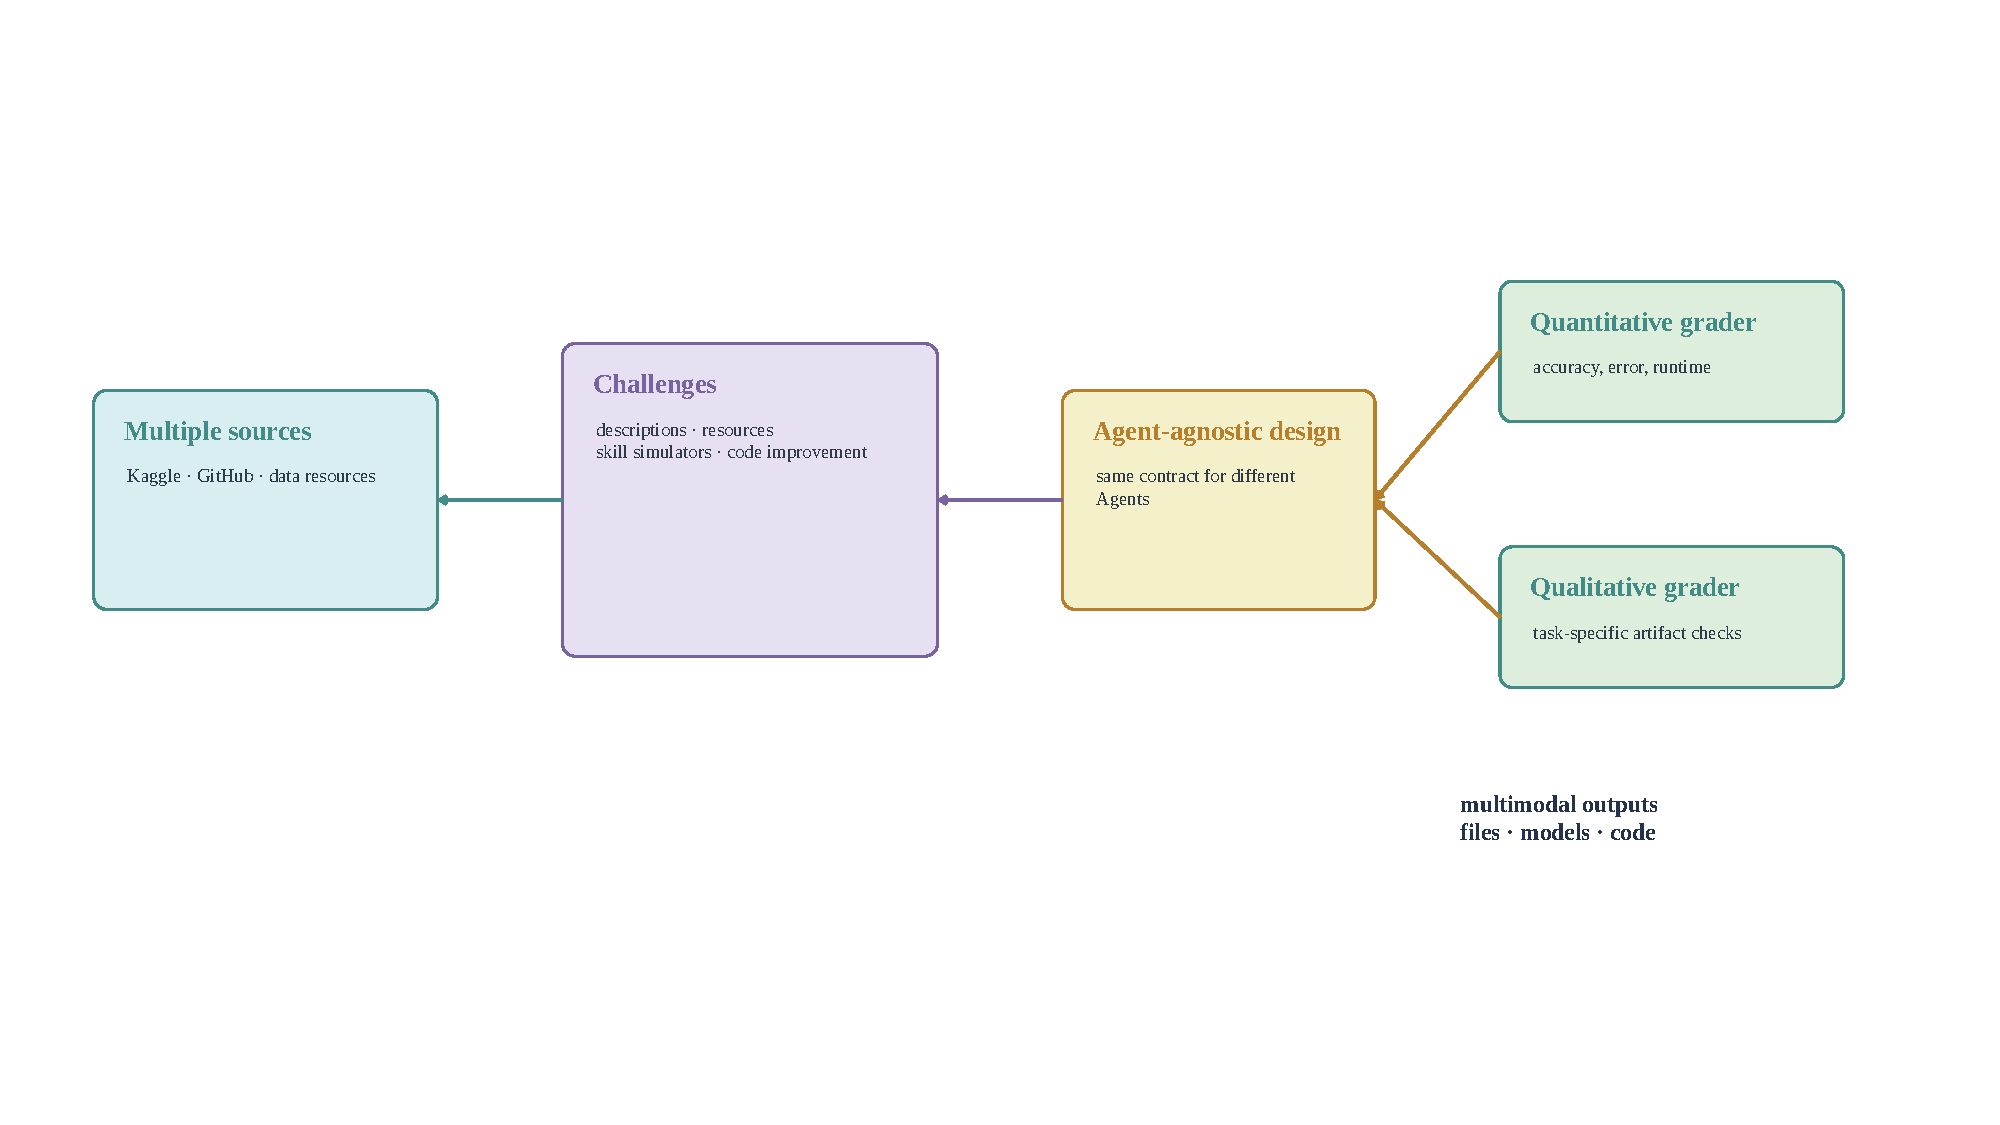
\includegraphics[width=0.78\linewidth]{artifacts/active/support_pdf/timeseriesgym_benchmark_native.pdf}
\caption{The benchmark view shows why task scores, executable artifacts, and evaluation traces must be read together when comparing Agents. Source: \citep{timeseriesgym2025}.}
\label{fig:benchmark-landscape}
\end{figure}


Forecasting suites measure horizon-respecting accuracy and probabilistic calibration. Anomaly and diagnosis suites measure detection, localization, root-cause attribution, and evidence. Augmentation suites measure fidelity and downstream utility. Decision-support studies measure policy, recommendation, or operational outcomes. TSQA and multimodal QA provide evidence for grounded temporal answers within the broader Agent contract.

\begin{table}[htbp]
\centering\scriptsize
\setlength{\tabcolsep}{1.5pt}
\noindent\textbf{What the benchmark table answers.} The table maps each resource to the part of the Agent contract that it can establish. Read across a row from resource to evidence type, then compare the rows: datasets and task metrics cover outcomes, while traces, tool interfaces, temporal splits, and recoverable artifacts cover the process around those outcomes. The pattern supports the conclusion that a unified Time-Series Agent benchmark must combine these layers.
\begin{tabularx}{\textwidth}{@{}L{0.17\textwidth}L{0.25\textwidth}L{0.24\textwidth}L{0.28\textwidth}@{}}
\toprule
\textbf{Resource} & \textbf{Coverage} & \textbf{Signal} & \textbf{Focus}\\
\midrule
TemporalBench \citep{temporalbench2026} & Four information settings spanning historical interpretation, context-free forecasting, contextual reasoning, and event-conditioned prediction. & Tests whether performance changes when temporal context is controlled. & Its protocol focuses on forecasting context and prediction outcomes.\\
TFRBench \citep{tfrbench2026} & Ten datasets across five domains with search--reasoning--verifier--forecasting--summary traces. & Separates forecast score from reasoning-trace quality using MASE and a reasoning judge. & Trace scoring depends on evaluator quality.\\
TraceBench \citep{tracebench2026} & Controlled root-cause attribution with noise, domain context, labeled examples, and direct versus programmatic submission. & Measures intervention-aware trajectories and attribution behavior. & Its protocol centers on controlled diagnostic environments.\\
TSAQA / MMTS-Bench \citep{tsaqa2026,mmtsbench2026} & Large temporal QA and multimodal QA collections with numerical, grounding, matching, and cross-modal tasks. & Measures language-facing temporal reasoning and evidence alignment. & Its coverage focuses on temporal QA and multimodal grounding.\\
TimeSeriesGym \citep{timeseriesgym2025} & ML-engineering challenges across domains, tasks, code, models, and submission artifacts. & Grades executable artifacts and combines quantitative and LLM-based evaluation. & Its coverage focuses on executable ML-engineering artifacts.\\
TSQBench \citep{tsqbench2026} & Data-quality diagnosis with multiple analytical tools, real-world datasets, and dimension-wise comparison. & Tests whether an Agent can inspect and adjudicate temporal data quality. & Its task contract centers on data quality.\\
\bottomrule
\end{tabularx}
\caption{Representative benchmark resources and the part of the Time-Series Agent contract that each can establish.}
\label{tab:benchmark-families}
\end{table}

These resources cover complementary parts of the Agent contract. TemporalBench and TFRBench emphasize contextual forecasting and reasoning traces; TraceBench controls diagnosis and interventions; TSAQA and MMTS-Bench measure temporal question answering and multimodal grounding; TimeSeriesGym evaluates executable ML-engineering artifacts; and TSQBench focuses on data-quality decisions. A unified suite would combine temporal availability, executable tools, evidence provenance, trace validation, and all four task families. Its coverage can be represented as a binary matrix over evaluation layers and benchmark resources:
\begin{equation}
  C_{\ell b}=\mathbb{1}\!\left[\text{resource }b\text{ measures layer }\ell\right],\qquad
  \ell\in\{\mathrm{GH},\mathrm{GTS},\mathrm{TSK},\mathrm{resource}\}.
  \label{eq:benchmark-coverage}
\end{equation}

\subsection{Role of QA within a Time-Series Agent benchmark}

\begin{figure}[htbp]
\centering
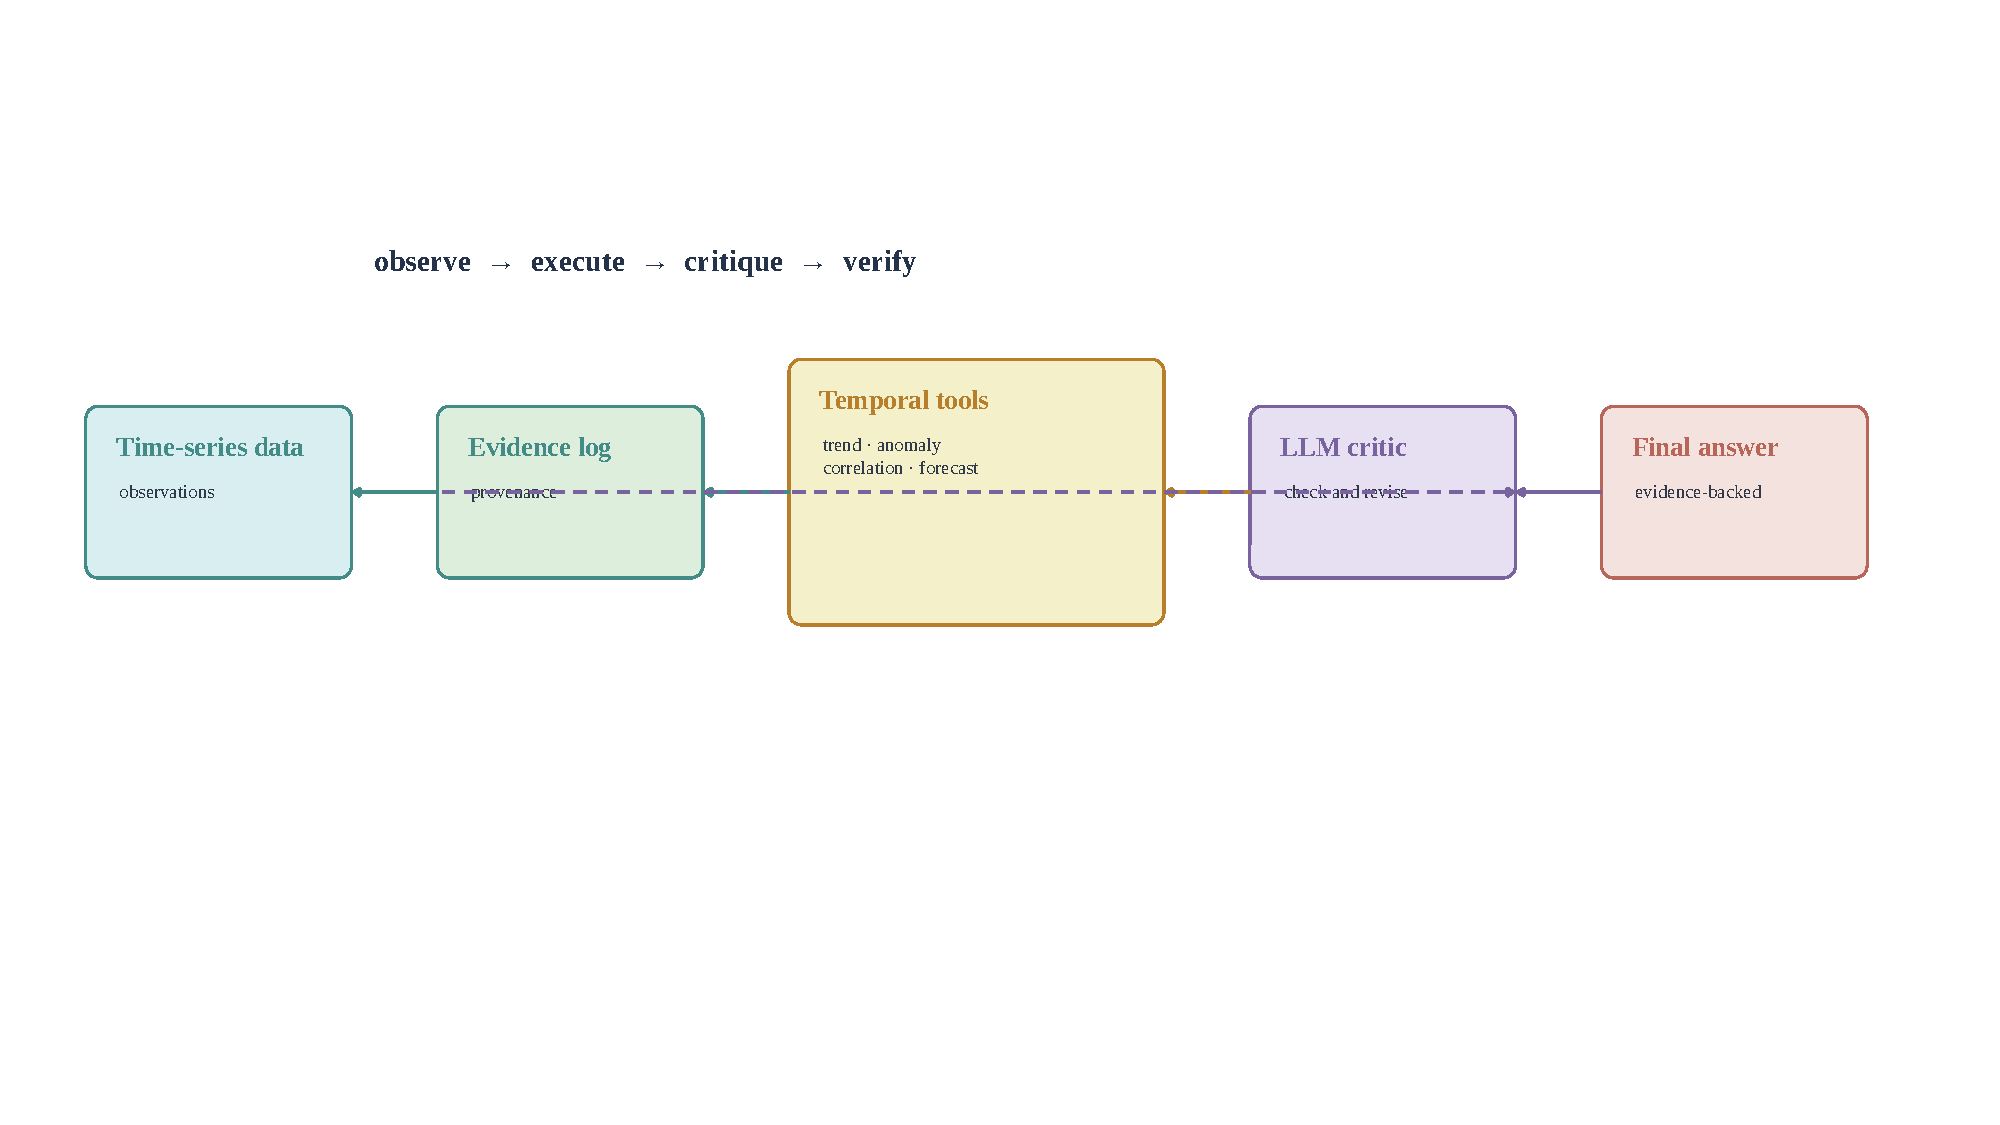
\includegraphics[width=0.78\linewidth]{artifacts/active/support_pdf/tsagent_trace_native.pdf}
\caption{The QA trace illustrates the language-facing part of evaluation: answers must remain grounded in temporal evidence and tool outputs. Source: \citep{tsagent2025}.}
\label{fig:benchmark-qa}
\end{figure}


QA resources evaluate temporal answers, evidence grounding, and selected numerical reasoning. They provide the language-facing part of evaluation; a complete Agent benchmark adds chronological validity, numerical fidelity, forecasting-horizon behavior, anomaly localization, augmentation quality, downstream decision utility, tool-call correctness, memory provenance, and validation traces.

\subsection{Infrastructure and the missing unified benchmark}

\begin{figure}[htbp]
\centering
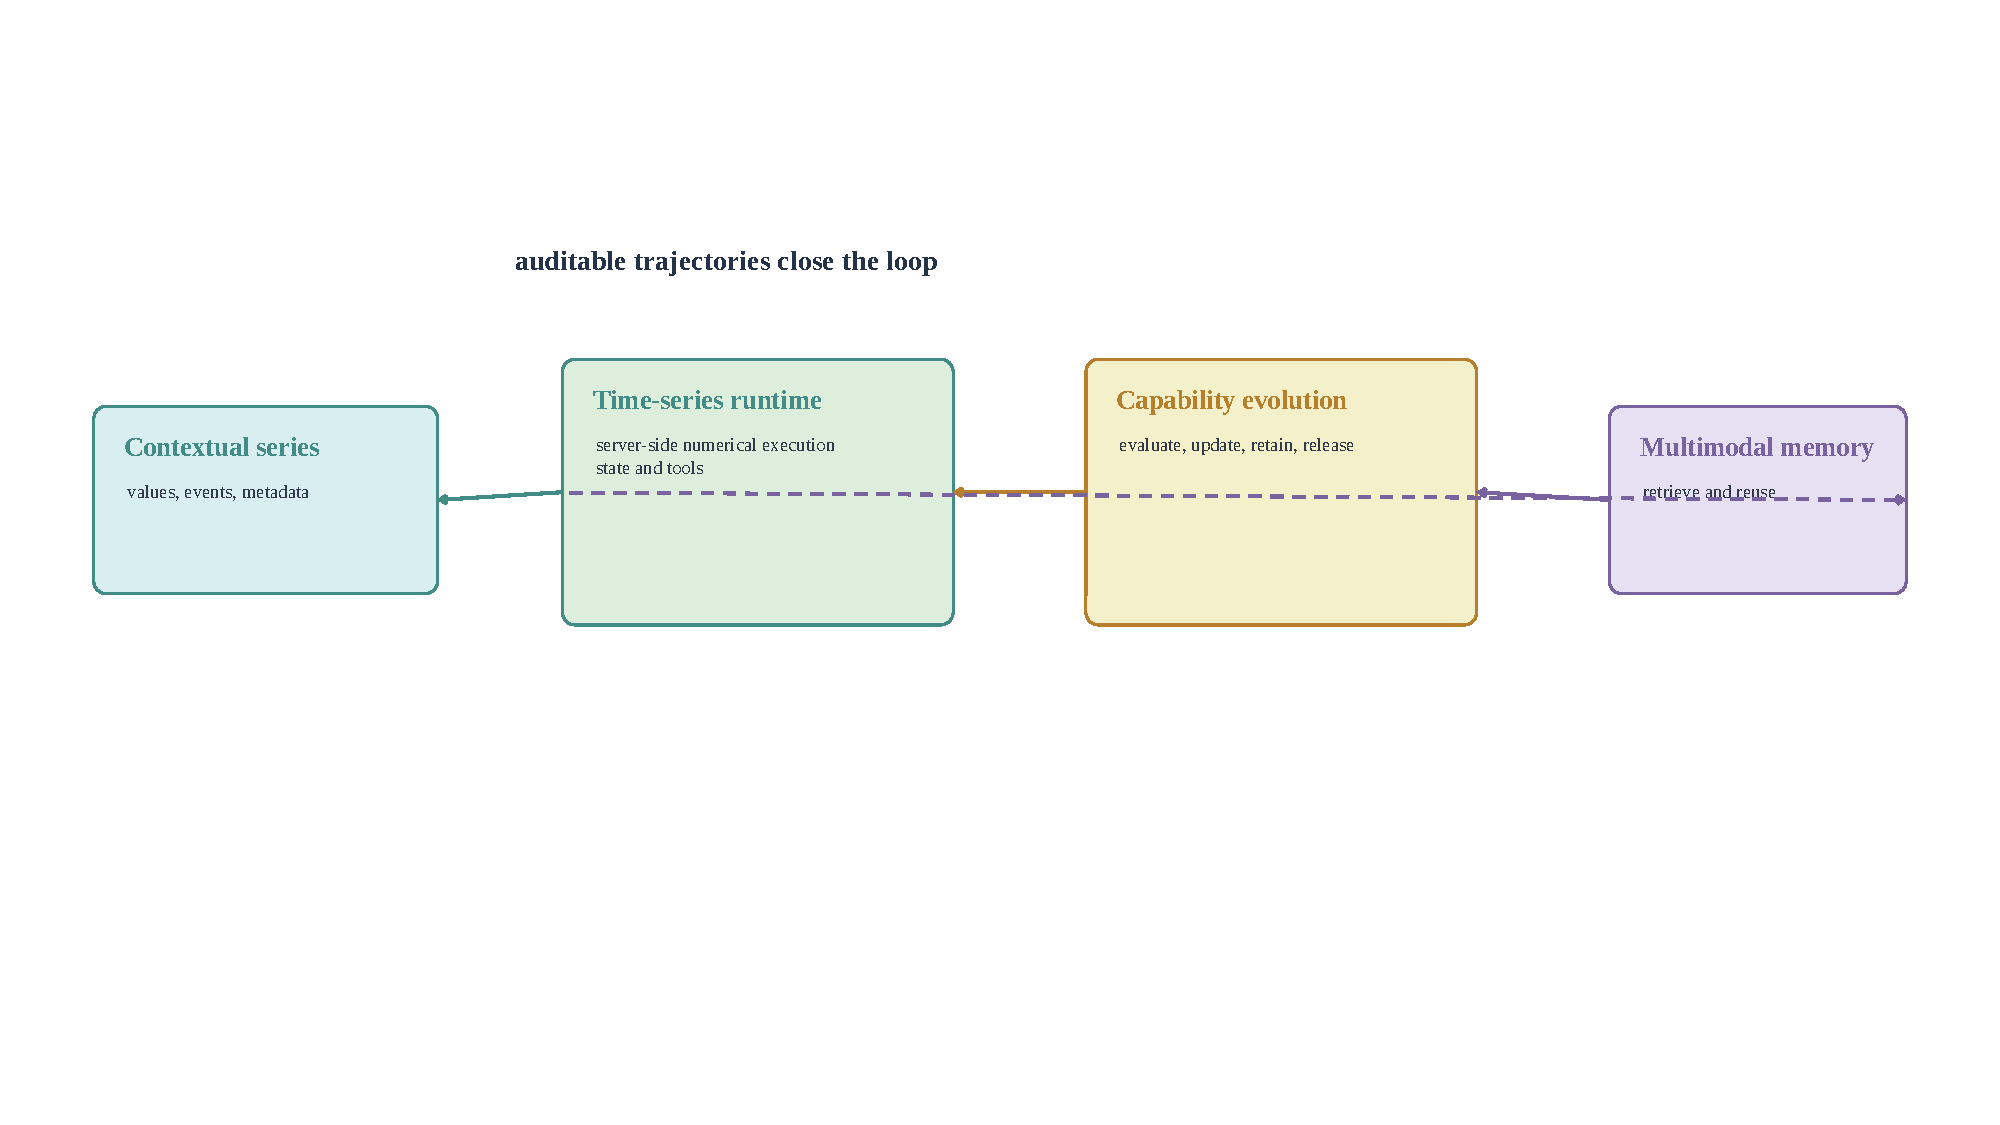
\includegraphics[width=0.78\linewidth]{artifacts/active/support_pdf/timeclaw_runtime_native.pdf}
\caption{The infrastructure view links tools, traces, experience, and validators into a reusable evaluation substrate. Source: \citep{timeclaw2026explore}.}
\label{fig:benchmark-infrastructure}
\end{figure}


FutureSim adds a replayable world-event environment in which an Agent can be evaluated under changing information and adaptive interaction, complementing dataset-fixed forecasting benchmarks \citep{futuresim2026}. WorldReasoner focuses on whether a forecasting Agent respects the information available at prediction time and whether its reasoning is valid, making temporal leakage and trace quality explicit benchmark targets \citep{worldreasoner2026}. TimeClaw, AION, TimeSeriesGym, and ModernTSF provide complementary infrastructure. ModernTSF contributes an agent-ready and reproducible forecasting substrate with model and dataset catalogs, callable interfaces, evidence, budgets, artifacts, and recoverable execution \footnote{ModernTSF repository: \url{https://github.com/Diaugeia/ModernTSF}.}. It provides an infrastructure case for the benchmark stack. A unified public suite would combine a time-indexed availability policy, executable temporal tools, trace and evidence validation, and task contracts across forecasting, augmentation, anomaly diagnosis, and decision support.

A reusable benchmark stack should therefore include a time-indexed workspace, explicit availability rules, executable temporal tools, trace and evidence schemas, validators, cases from all four task families, and cost, failure, and revision logs. These requirements connect the infrastructure chapter to the open problems below.

\subsection{Selecting a benchmark for a new scenario}

\begin{figure}[htbp]
\centering
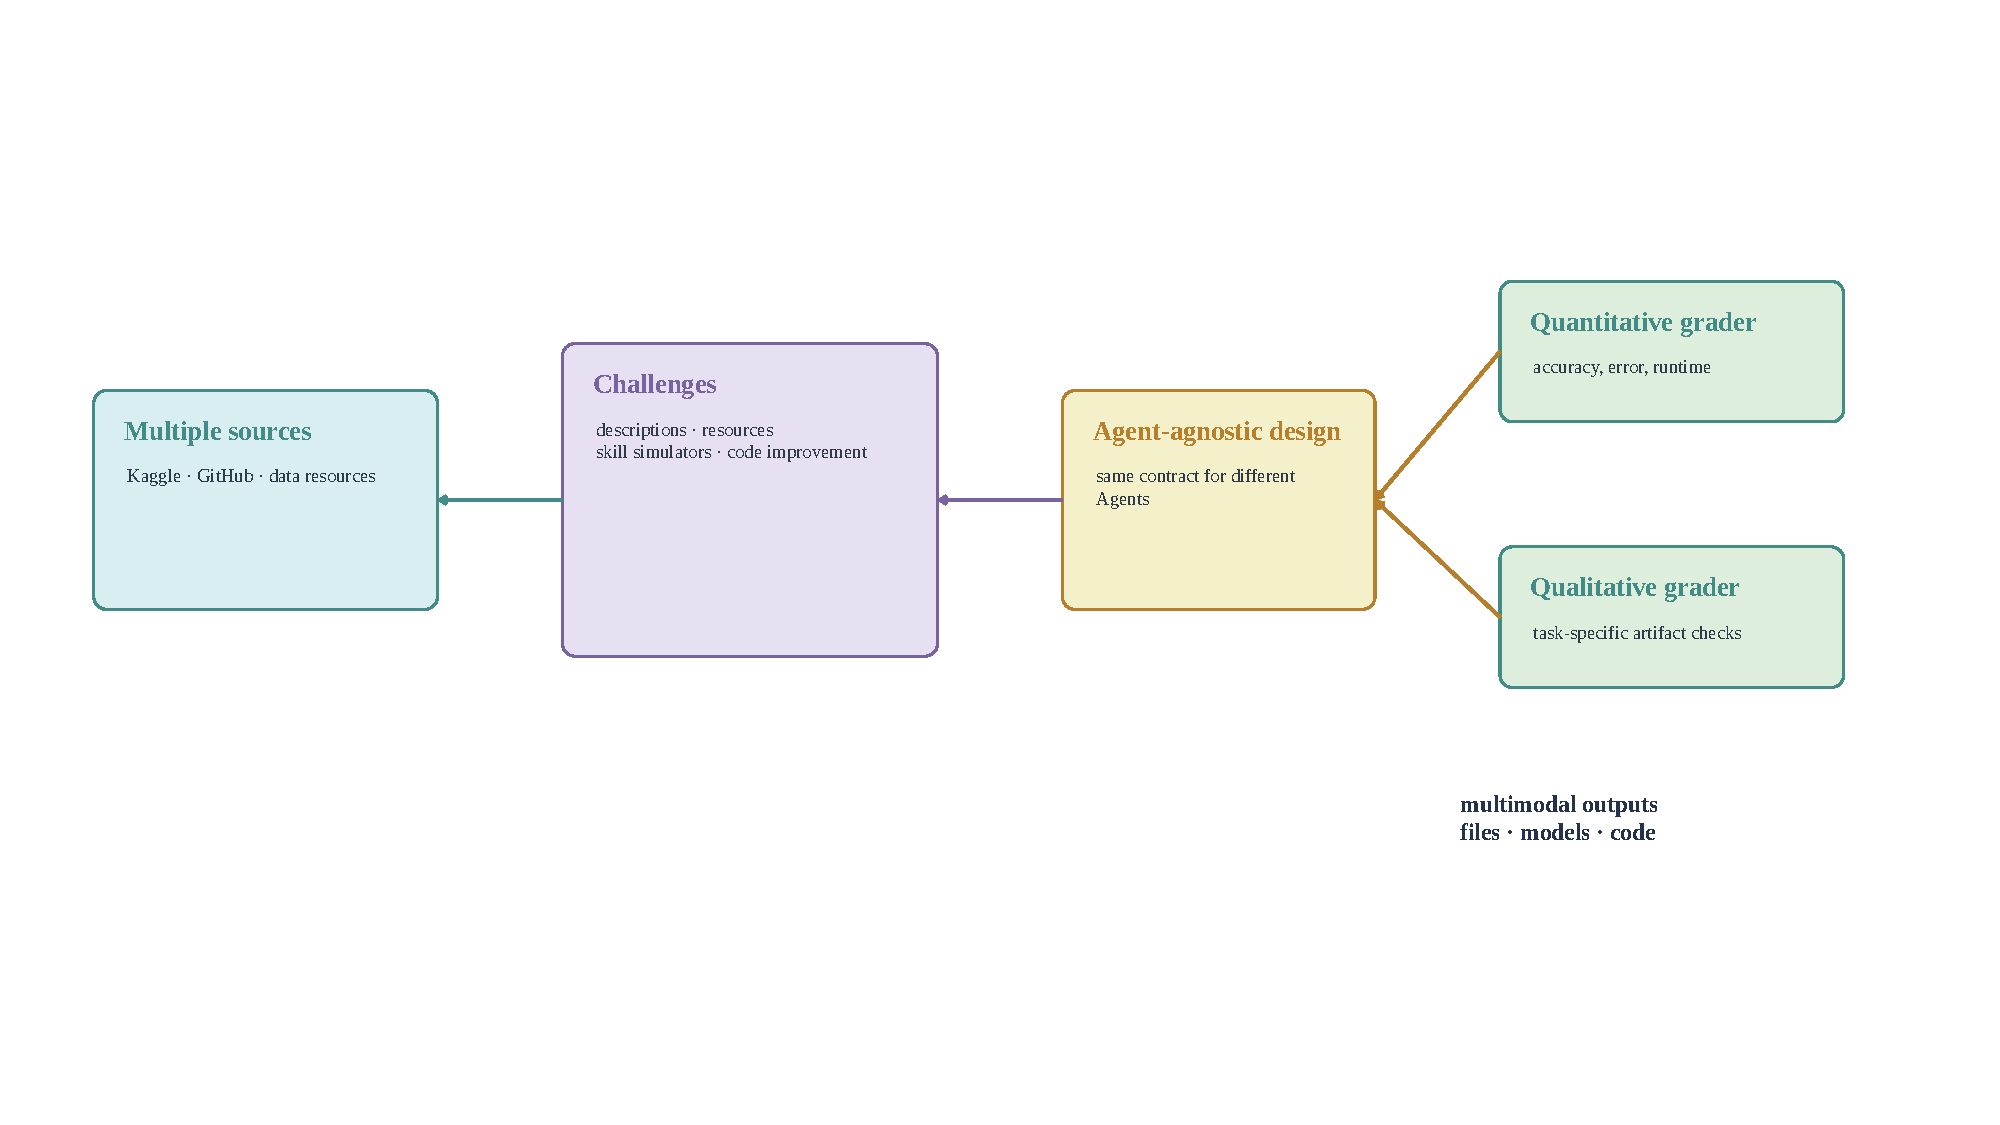
\includegraphics[width=0.78\linewidth]{artifacts/active/support_pdf/timeseriesgym_benchmark_native.pdf}
\caption{The benchmark-selection view emphasizes coverage of process, temporal contract, task outcome, and resource behavior rather than a single score. Source: \citep{timeseriesgym2025}.}
\label{fig:benchmark-selection}
\end{figure}


A benchmark should be selected by matching its coverage to the task contract, rather than by choosing the dataset with the most convenient score. For a new scenario, first require an availability policy and temporal split; then require the tools, evidence, and validators needed by the workflow; finally require task metrics and a decision or review signal when the output will guide action. A resource can be strong on one layer and silent on another, so a benchmark suite may combine several resources while preserving one episode record and one evaluation vector.

\begin{equation}
  b^{\star} = \underset{b\in\mathcal{B}}{\operatorname{argmax}}\; \sum_{\ell} w_{\ell} C_{\ell b},
  \qquad \sum_{\ell}w_{\ell}=1,
  \label{eq:benchmark-selection}
\end{equation}

Here $C_{\ell b}$ is the coverage indicator used above and $w_{\ell}$ is the importance of evaluation layer $\ell$ for the scenario. Forecasting deployments assign more weight to horizon and calibration; diagnosis assigns more weight to localization and evidence; decision support assigns more weight to utility, cost, and review authority. This turns benchmark selection into an explicit design decision that can be audited and revised.
\section{Open Problems and Focused System Analyses}

\subsection{Reusable temporal infrastructure}

\begin{figure}[htbp]
\centering
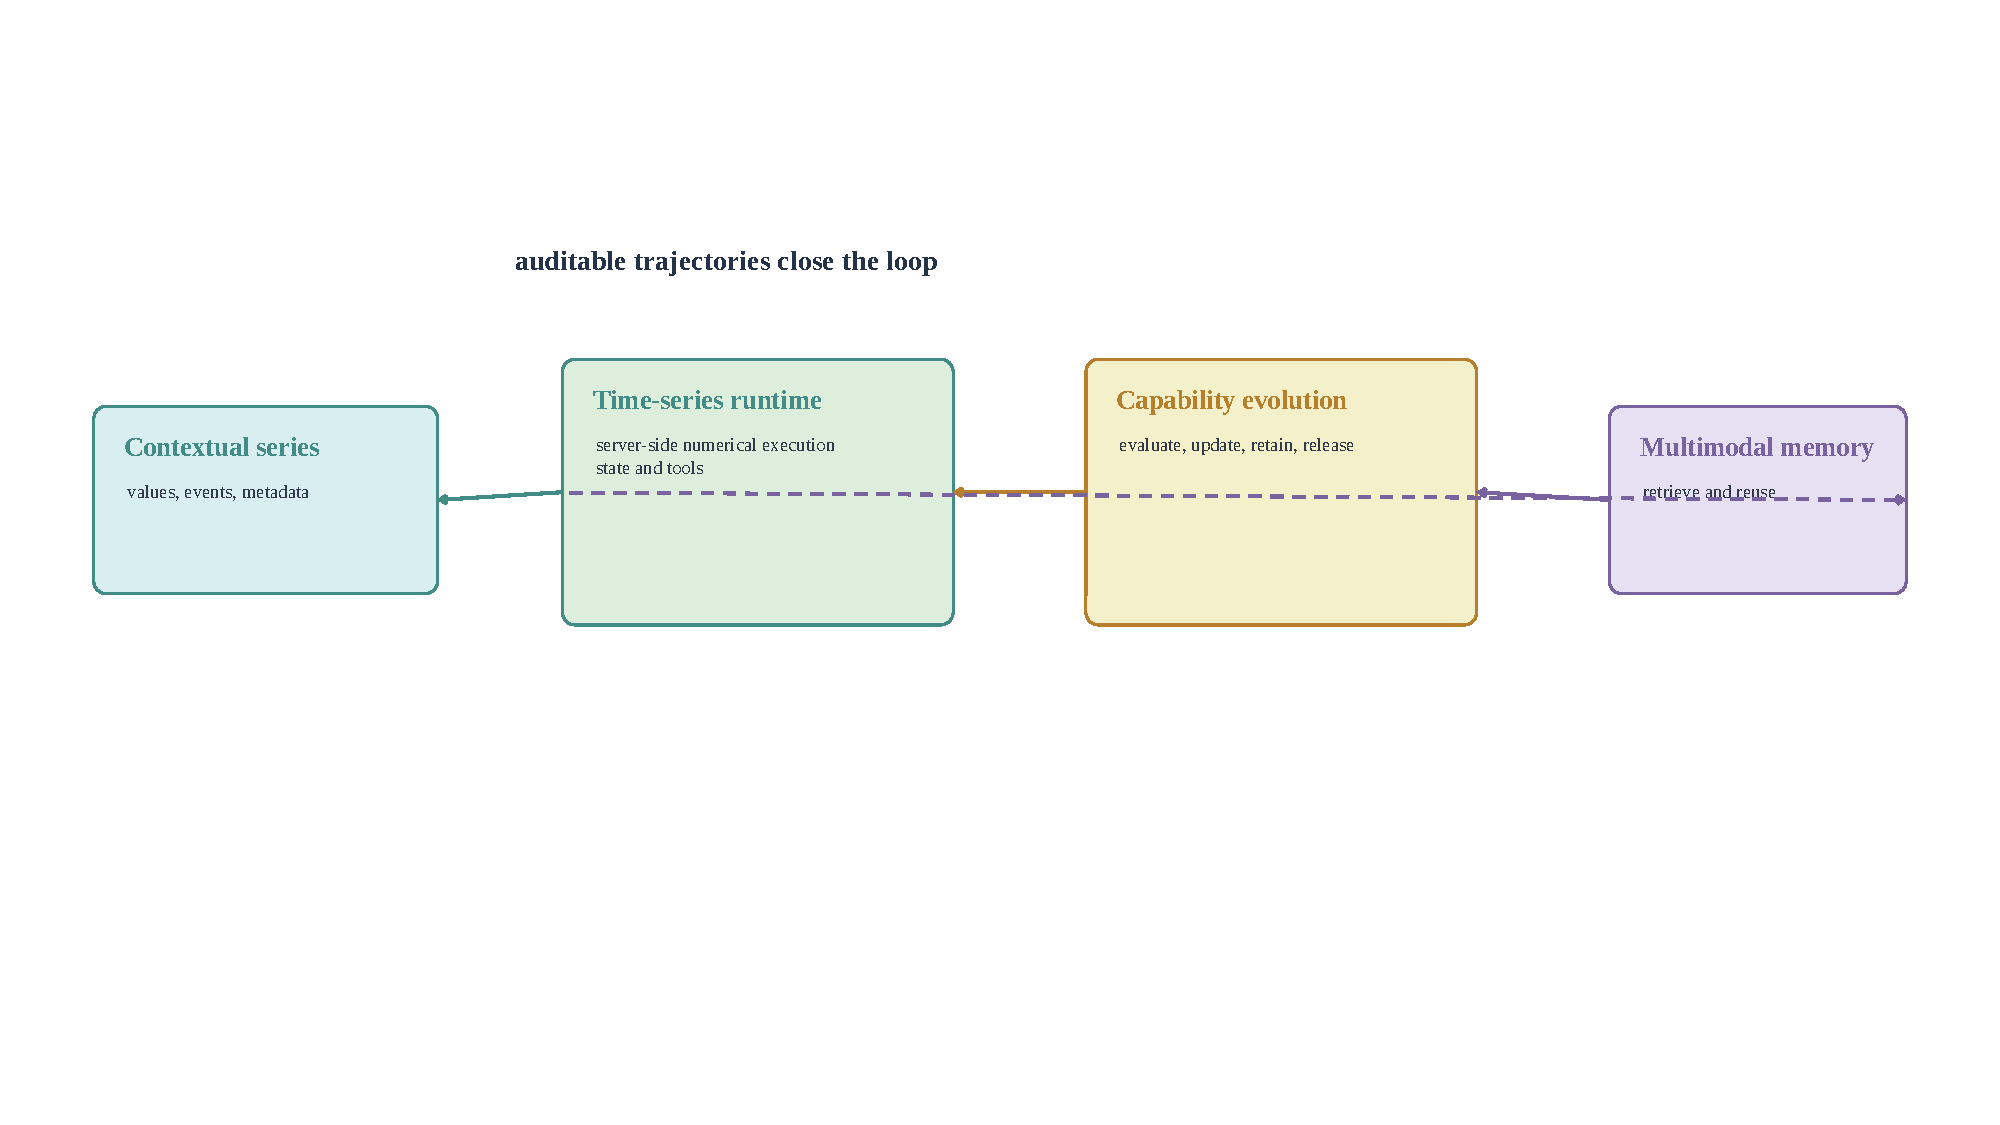
\includegraphics[width=0.78\linewidth]{artifacts/active/support_pdf/timeclaw_runtime_native.pdf}
\caption{The workspace view shows how data, tools, traces, validators, and artifacts are bound to one point-in-time state. Source: \citep{timeclaw2026explore}.}
\label{fig:open-infrastructure}
\end{figure}


Time-Series Agents need shared workspaces, temporal tool contracts, evidence schemas, validators, and reproducible execution. ModernTSF, TimeClaw, AION, and related projects show complementary pieces of this stack. A reusable workspace binds data, tools, traces, and validators to one point-in-time state:
\begin{equation}
  \mathcal{W}_{\tau}=\left(\mathcal{D}_{\leq\tau},\mathcal{T},\mathcal{R}_{\tau},\mathcal{V},\mathcal{A}_{\tau}\right),
  \qquad \mathcal{R}_{\tau}=\operatorname{Run}(\mathcal{W}_{\tau},\pi_{\theta}).
  \label{eq:infrastructure-workspace}
\end{equation}

\subsection{Open problems}

The module ledger makes these open problems explicit. Each card separates the claim, module, task contract, and evidence, so gaps appear as missing or weakly supported regions in the research map. Across the reviewed cards, the clearest gaps occur at the interfaces between layers: model-side temporal understanding is rarely connected to auditable Harness state; reusable temporal modules are often evaluated through a single task; and task-specific systems seldom report decision feedback, revision behavior, or deployment cost. New papers can therefore be assessed by asking which card field or module they strengthen and which previously unsupported contract they make measurable.

\noindent\textbf{Temporal and numerical faithfulness.} Agents need typed temporal operations, unit-aware representations, chronology guards, and end-to-end fidelity checks. A textual explanation is reliable when tools preserve frequency, precision, and forecast-origin constraints. Future systems should validate numerical and temporal invariants at every interface alongside the final answer. For an operation $o$ applied at time $\tau$, the invariant is
\begin{equation}
  \operatorname{Faithful}(o;\tau)=\mathbb{1}\!\left[\operatorname{Time}(o)\subseteq\mathcal{I}_{\tau}\;\wedge\;\operatorname{Unit}(o)=1\;\wedge\;\operatorname{Value}(o)=1\right].
  \label{eq:open-faithfulness}
\end{equation}

\noindent\textbf{Context retrieval and memory with temporal provenance.} Retrieved events and episodic memories need availability-time provenance, expiry, regime awareness, and replayable audits. This problem links GTS memory to evaluation: an Agent should be able to reconstruct exactly which event, revision, or prior trajectory was visible when a decision was made. A replayable retrieval is defined by its query, availability boundary, and returned evidence:
\begin{equation}
  \operatorname{Replay}(q,\tau)=R_{\psi}\left(\mathcal{M}_{\leq\tau},q\right),
  \qquad \operatorname{Prov}(m)=\left(t_{\mathrm{event}},t_{\mathrm{avail}},t_{\mathrm{rev}}\right).
  \label{eq:open-memory-provenance}
\end{equation}

\noindent\textbf{Interface standardization.} Shared schemas for temporal workspaces, tools, traces, and validators would make systems composable and comparable. A common contract aligns as-of policies, window semantics, and failure handling across Agents. A standard temporal tool schema can be represented as
\begin{equation}
  \mathcal{S}_{\mathrm{tool}}=\left(n,\operatorname{Args},\operatorname{Ret},\operatorname{Time},\operatorname{Perm},\operatorname{Fail}\right).
  \label{eq:open-tool-schema}
\end{equation}

\noindent\textbf{Self-evolving components.} Tool, policy, memory, and workflow updates require regression checks under temporal shift. Capability evolution should preserve previous generations when a new component fails held-out temporal checks, and should record the evidence that justified promotion. For a candidate component $\phi'$, promotion requires improvement on held-out temporal episodes without violating a regression bound:
\begin{equation}
  \operatorname{Promote}(\phi')=\mathbb{1}\!\left[\Delta E_{\mathrm{heldout}}(\phi')\geq\delta \;\wedge\; \Delta E_{\mathrm{regress}}(\phi')\leq\epsilon\right].
  \label{eq:open-evolution}
\end{equation}

\noindent\textbf{Decision-centric evaluation.} Future benchmarks should connect predictive or diagnostic evidence to action quality, cost, uncertainty, and accountability. Prediction informs action; an Agent benchmark should measure whether a forecast or diagnosis changes a decision appropriately under explicit constraints, alongside prediction accuracy. A decision episode couples the predictive distribution to an action utility:
\begin{equation}
  a_{\tau}^{\star}=\arg\max_{a\in\mathcal{A}}\mathbb{E}\left[U(a,Y_{\tau+1})\mid\mathcal{I}_{\tau}\right]-\lambda\operatorname{Cost}(a).
  \label{eq:open-decision-utility}
\end{equation}

\subsection{Focused system analyses}

\noindent\textbf{ChatTS: changing the LLM side.} ChatTS equips a language model with temporal values and attributes through a multimodal input pipeline. Its attribute selector, synthetic time-series/text generator, evolution-instruct stage, and multimodal model align numerical series with language supervision \citep{chatts2025}. In our ledger this is an LLM-side contribution with a General Time-Series Harness binding: the learned alignment is reusable across temporal questions, while the dialogue and reasoning tasks provide task-specific instantiations. The central evidence is the change in what the LLM can represent and explain, together with the synthetic-data assumptions shown in Fig.~\ref{fig:chatts-overview}.

\noindent\textbf{TimeClaw: making temporal semantics executable.} TimeClaw turns the GTS boundary into a runtime: numerical execution remains server-side, temporal tools evolve through an evaluated toolbox, and solution trajectories remain auditable and reusable \citep{timeclaw2026explore}. Its method is an explicit Explore--Compare--Distill--Reinject loop. For a task instance $x$, candidate executions are scored by task loss and the best valid trajectory is selected:
\begin{equation}
  q(\pi_k;x)=-L_{\tau}(\widehat{y}_k,y^{\star}),\qquad
  \pi^{\star}(x)=\arg\max_{\pi_k\in\Pi_{\mathrm{valid}}(x)}q(\pi_k;x).
  \label{eq:timeclaw-compare}
\end{equation}
The selected execution is summarized, cleaned to remove answer leakage and non-transferable control text, and distilled into an external experience state:
\begin{equation}
  n_x=\operatorname{Summarize}\!\left(x,\Pi(x),\{q(\pi_k;x)\}_{k=1}^{K},\pi^{\star}(x)\right),\quad
  e_x=\operatorname{Clean}(n_x),\quad
  A_s^{(m+1)}=\operatorname{Distill}\!\left(A_s^{(m)},e_x\right).
  \label{eq:timeclaw-distill}
\end{equation}
These equations capture the paper's concrete contribution: execution quality, rather than completion alone, determines which temporal tool trajectory becomes reusable experience \citep{timeclaw2026explore}.

\noindent\textbf{How the open-problem map is derived.} Each node starts from a missing or weakly evidenced Paper Card field and is connected to the Harness layer where the gap appears. Read from left to right: model-side temporal understanding, runtime state and tools, task contracts, evaluation infrastructure, and deployment feedback. The map turns the evidence ledger into research questions rather than a free-standing list of future work.

\begin{figure}[htbp]
\centering
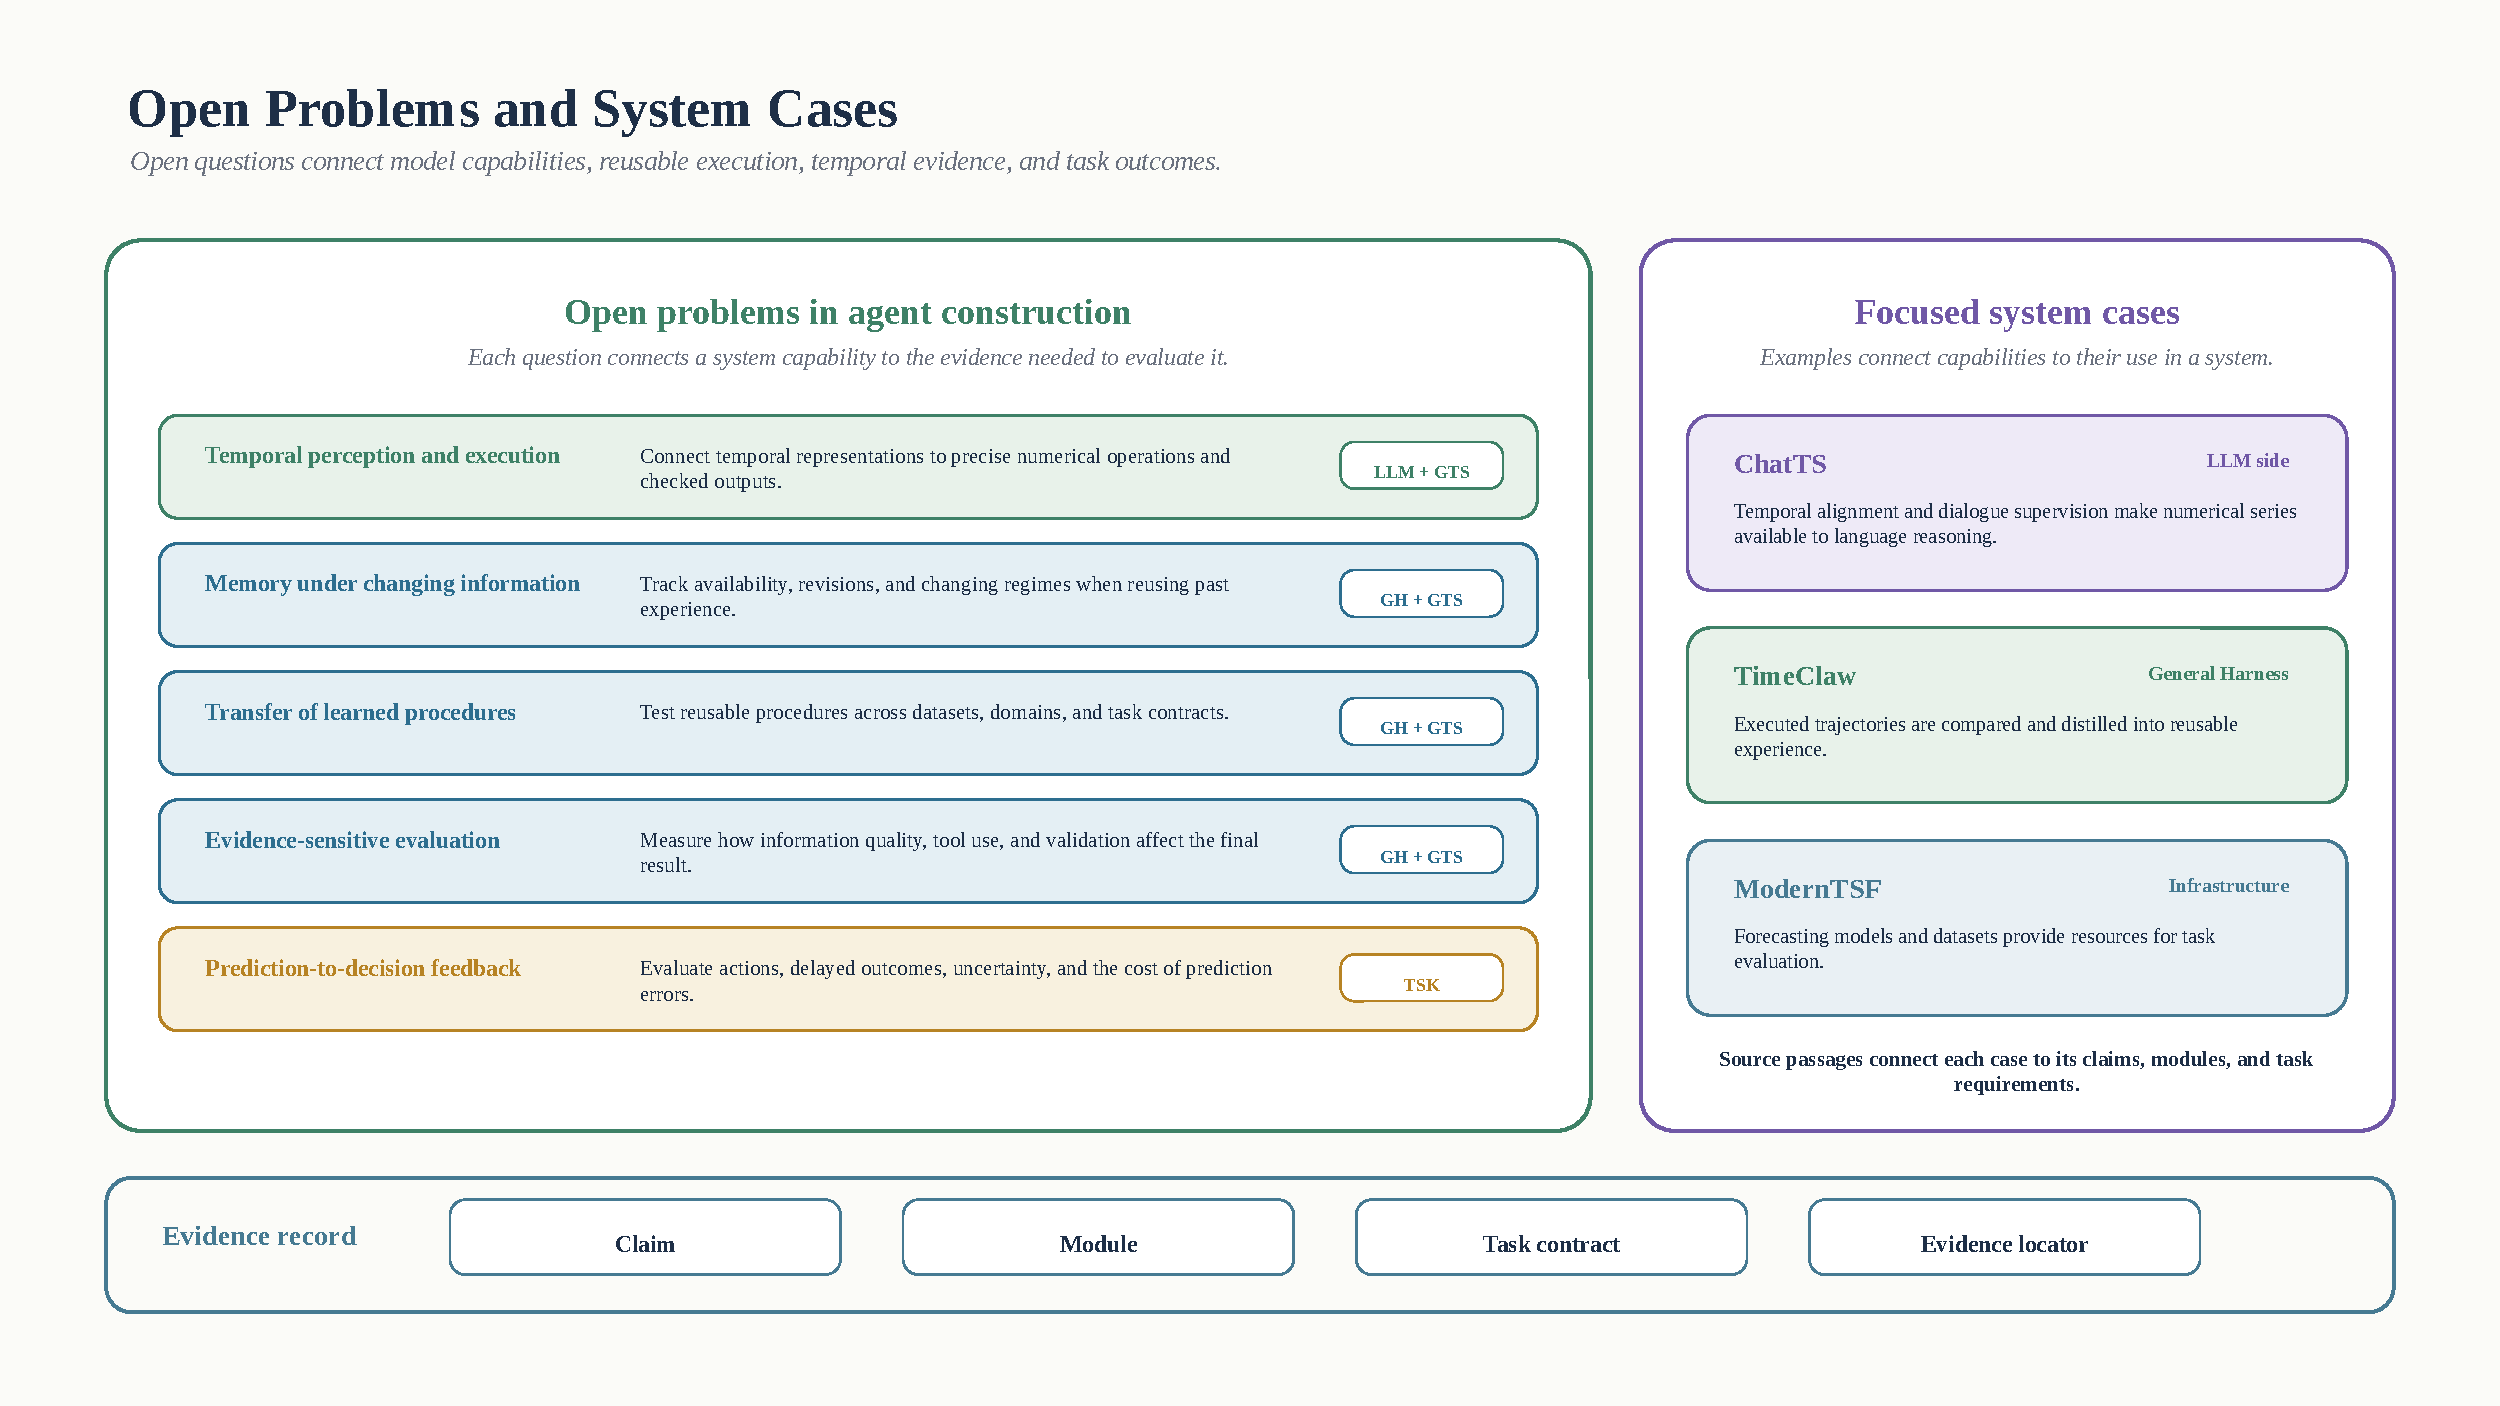
\includegraphics[width=0.98\linewidth]{artifacts/active/Figure8_open_problems_native.pdf}
\caption{Open problems and focused system cases. The ledger links each gap to a Harness layer and records representative LLM-side, temporal-runtime, and infrastructure contributions.}
\label{fig:open-problems-cases}
\end{figure}

\noindent\textbf{ModernTSF: infrastructure and reproducibility.} ModernTSF represents the infrastructure contribution: callable model and dataset interfaces, evidence, budgets, artifacts, and recoverable execution provide a foundation for reproducible Agent evaluation \footnote{ModernTSF repository: \url{https://github.com/Diaugeia/ModernTSF}.}. Its role in this survey is to specify what a benchmark must make executable and inspectable: data and model identity, tool inputs and outputs, budgets, intermediate artifacts, and recoverable failures. It complements the benchmark resources in Table~\ref{tab:benchmark-families} and supplies the infrastructure layer for a unified cross-task evaluation protocol. The reproducible record is
\begin{equation}
  \mathcal{A}_{\mathrm{run}}=\left(\operatorname{ID}_{\mathcal{D}},\operatorname{ID}_{\mathcal{M}},\omega_{1:K},\operatorname{Artifacts},\operatorname{Budget},\operatorname{Failures}\right).
  \label{eq:moderntsf-record}
\end{equation}

\section{Conclusion}

A Time-Series Agent is built by combining an LLM, a General Harness, and a Time-Series Harness Module. The practical path is to begin with a scenario and task contract, select the runtime mechanisms that make the workflow executable, add temporal semantics where chronology and provenance matter, and specialize the final output contract for the task at hand. The four task families show how the same construction can support forecasting, augmentation, anomaly diagnosis, and decision support.

The evaluation path follows the same structure. A useful benchmark records the information boundary, execution trace, temporal checks, task outcome, resource behavior, and, when the result guides action, the decision utility and review outcome. This construction view gives practitioners a way to design a new Time-Series Agent and gives researchers a common coordinate system for adding new capabilities, tasks, and benchmarks.
% Keep the references between the main conclusion and the audit appendix.
\clearpage
\reftitle{References}
\bibliography{TS_AGENT_HARNESS_SURVEY}

\clearpage
\appendix
\section{Module-Level Contribution Ledger}
\label{app:full-ledger}
The machine-readable JSON ledger is a central research artifact of this survey. It records, for each work, the bibliographic identity, publication date, claim, source locator and quotation, LLM-side contribution, General Harness dimensions, General Time-Series Harness dimensions, Task-Specific Harness dimensions, task family, work type, and review status. The ledger is extensible: each new paper adds a supported module-level record to the construction hierarchy. The human-readable profiles below expose the same information in a form suitable for inspection.

\subsection{Paper Card schema}

\begin{figure}[htbp]
\centering
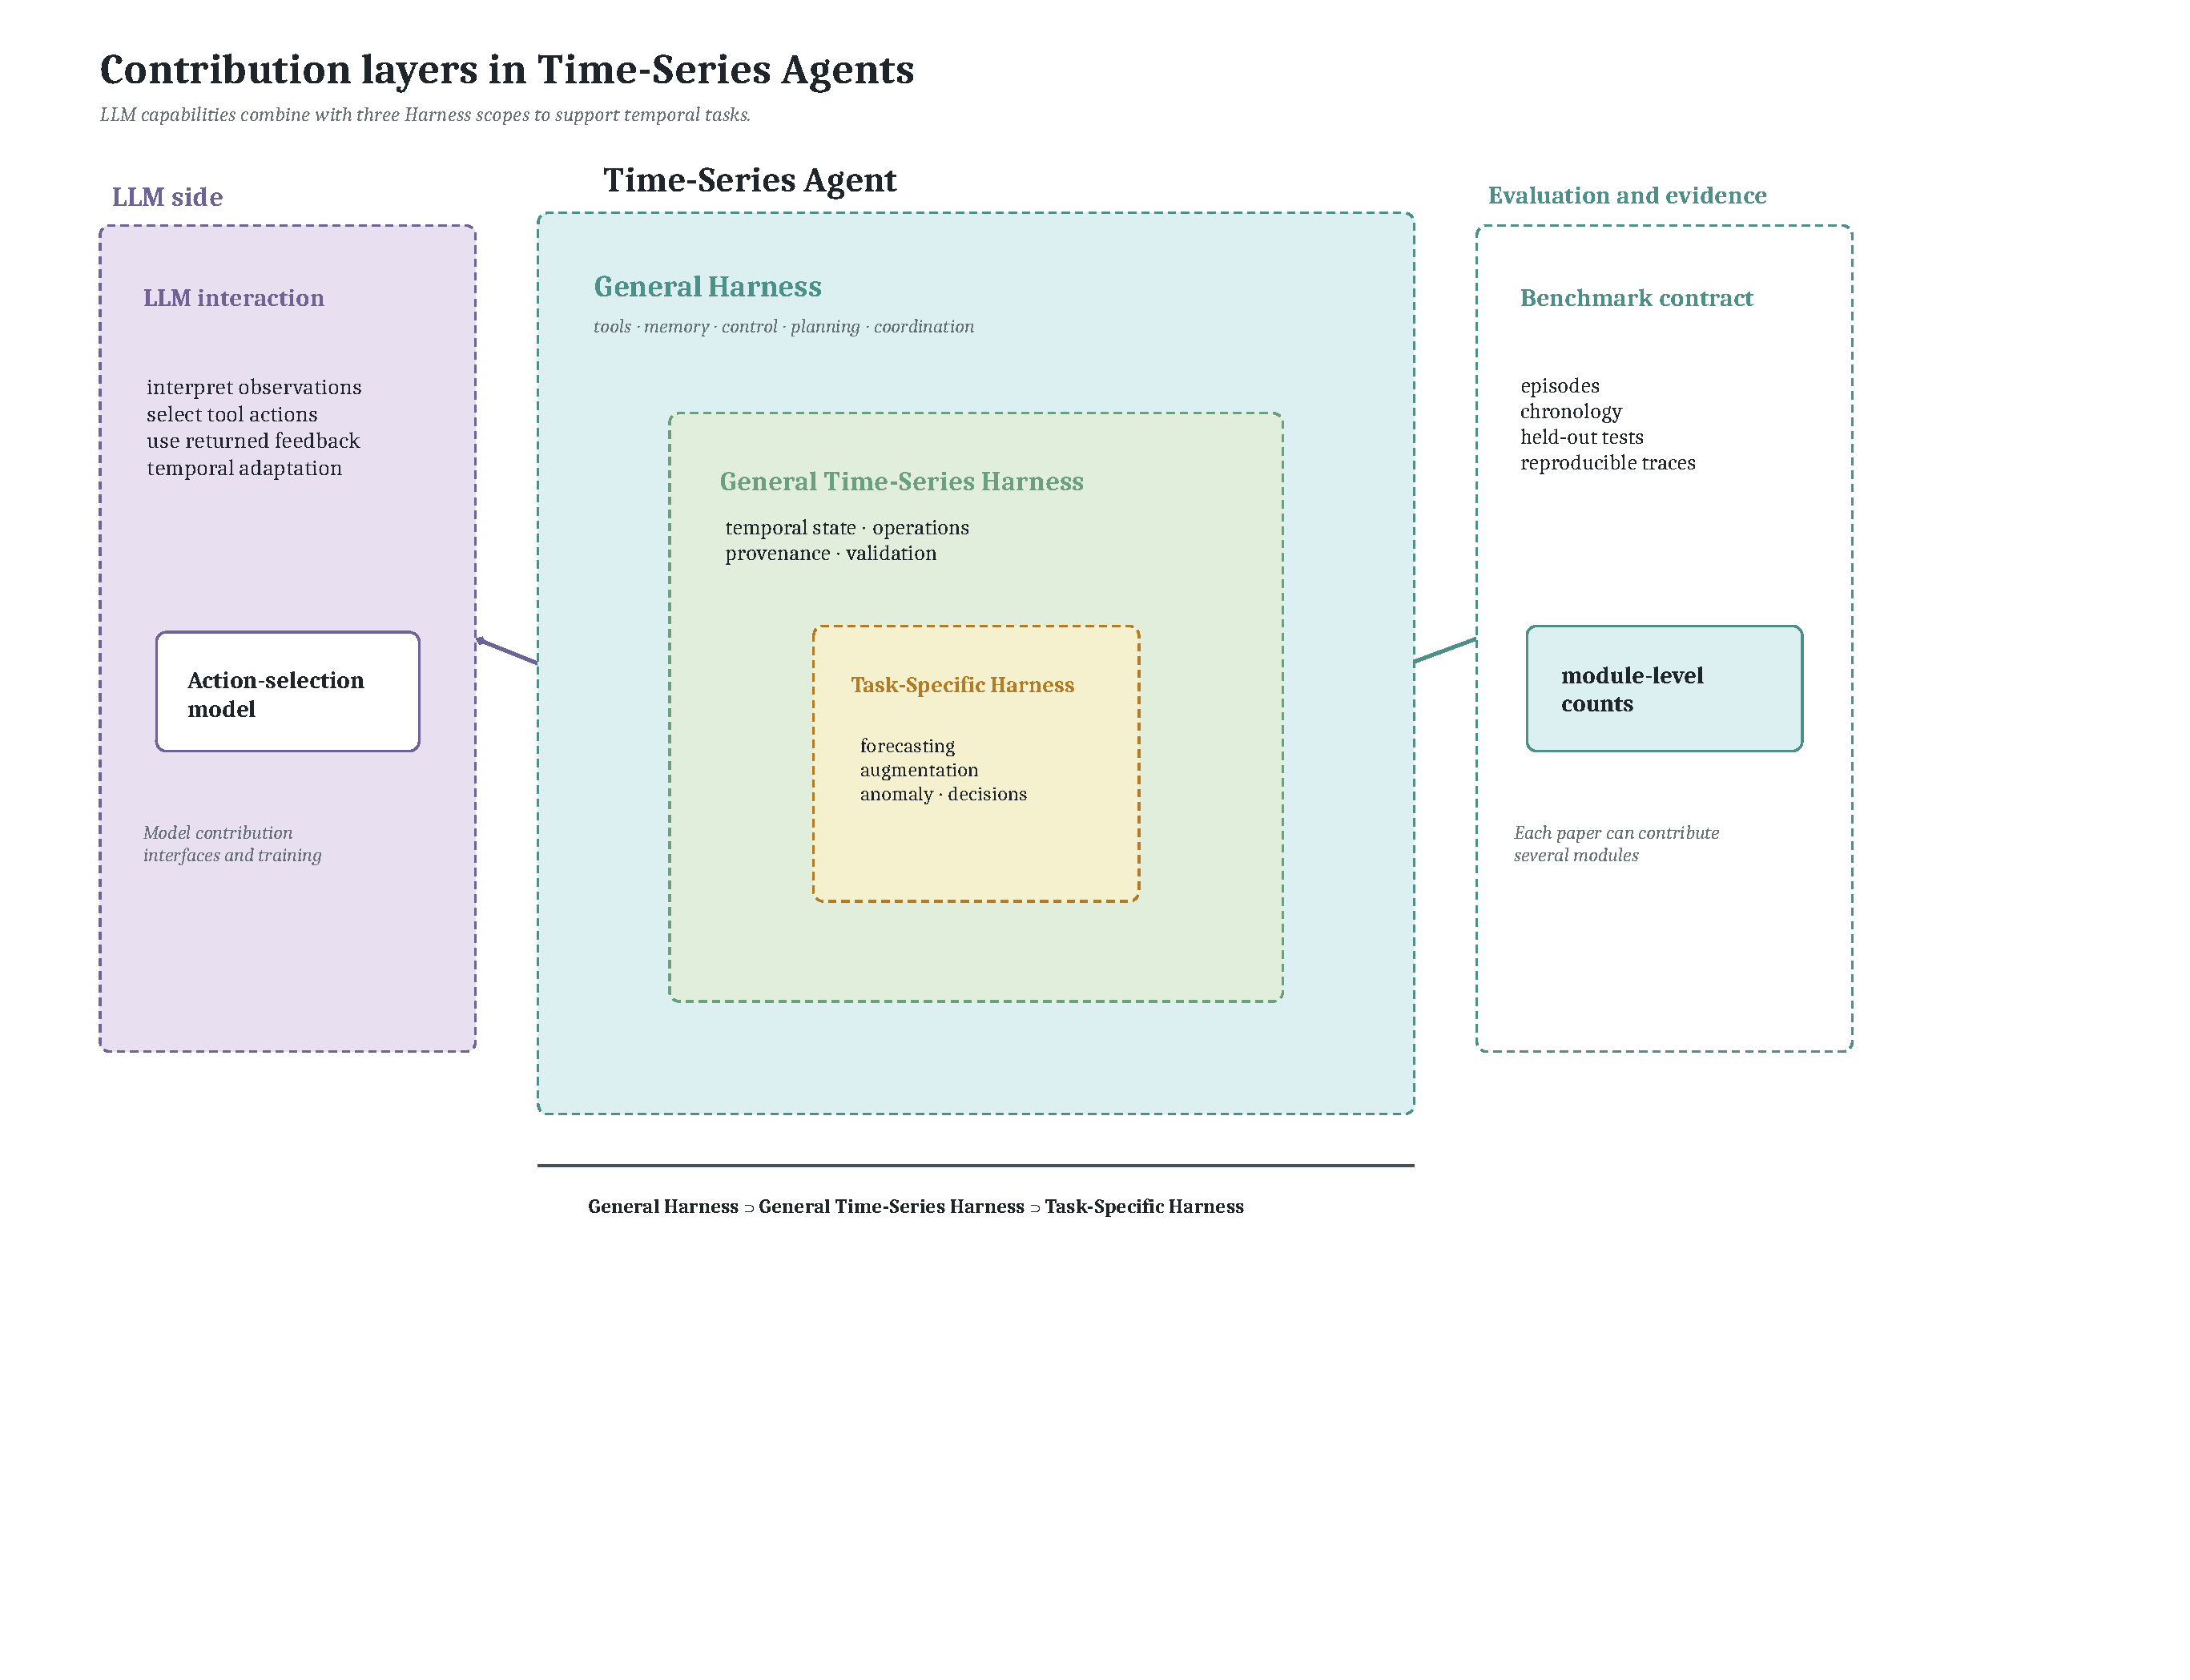
\includegraphics[width=0.78\linewidth]{artifacts/active/Figure3_construction_rsi_adapted.pdf}
\caption{The construction diagram is the visual key for the Paper Card fields: identity and claim are linked to contribution modules, task contracts, and evaluation evidence.}
\label{fig:app-card-schema}
\end{figure}

\label{app:paper-card}
A Paper Card is the evidence unit used to maintain the survey. It keeps bibliographic identity, the paper's own claim, source evidence, module contributions, task contract, evaluation evidence, and review status in one record. The card is multi-label: one work may contribute to the LLM side and to several Harness modules. Aggregate Harness plots apply the deepest-layer rule to each concrete module, while the inclusive evidence fields remain available for audit.

\begin{tcolorbox}[
  colback=surveyCard,
  colframe=surveyBlue!55!black,
  boxrule=0.8pt,
  arc=5pt,
  left=10pt,
  right=10pt,
  top=8pt,
  bottom=8pt,
  title=\textbf{Paper Card fields},
  fonttitle=\sffamily\bfseries,
  coltitle=surveyBlue!80!black
]
\small
\begin{tabularx}{\linewidth}{@{}>{\sffamily\bfseries}p{0.22\linewidth}X@{}}
Identity & Authors, year, landing page, BibTeX key, PDF, and source status.\\
Claim & The central claim and concrete contribution stated by the work.\\
Evidence & Page or section locator, quotation, figure or table, and verification status.\\
Modules & LLM-side capability, General Harness, General Time-Series Harness, and Task-Specific Harness entries.\\
Task contract & Forecasting, augmentation, anomaly diagnosis, decision support, or another supported task family.\\
Evaluation & Process validity, temporal-contract checks, task metrics, and deployment or decision evidence.
\end{tabularx}
\end{tcolorbox}

We construct each card in four passes: verify the work identity and publication record; extract the paper's claim with a page- or section-level quotation; code the concrete mechanisms it changes; and record task and evaluation evidence. A mechanism that transfers across temporal tasks is coded as General Time-Series Harness, a task-bound state, action, reward, or validator as Task-Specific Harness, and a domain-independent runtime mechanism as General Harness. The card can therefore support citation management, module tables, cumulative plots, and open-problem analysis without assigning a paper to a single mutually exclusive class.

\begin{tcolorbox}[
  colback=surveyCard,
  colframe=surveyBlue!40!black,
  boxrule=0.6pt,
  arc=4pt,
  left=8pt,
  right=8pt,
  top=6pt,
  bottom=6pt
]
\small
\textbf{Current ledger snapshot.} The database contains \textbf{138} Paper Cards, including 136 production-Bib records and 2 repository-only resources. 22 records have paper-verified claim summaries. Module-level review currently covers 9 works and 19 individually located modules; the remaining records retain candidate classifications. Task memberships comprise 82 forecasting/prediction, 19 augmentation/synthesis, 24 anomaly/diagnosis, and 27 decision-support records. 14 records carry LLM-side annotations. A record may have several task memberships.
\end{tcolorbox}

\begin{table}[htbp]
\centering\small
\noindent\textbf{Why this appendix table is retained.} The table is the compact decoding key for the Paper Card hierarchy. It tells the reader which question each layer answers before the full profiles are shown; the nesting also explains why aggregate plots assign a concrete module to its deepest applicable layer.
\begin{tabularx}{\textwidth}{@{}lX@{}}
\toprule
\textbf{Level} & \textbf{Question}\\
\midrule
General Harness & What runtime mechanisms turn an LLM into an agent, independently of time-series assumptions?\\
Time-Series Harness Module & What temporal objects, operations, context bindings, and validation interfaces make the runtime suitable for time-series analysis?\\
General Time-Series Harness & Which temporal mechanisms remain reusable when the downstream time-series task changes?\\
Task-Specific Harness & Which mechanisms are tied to a concrete task contract, such as a forecasting horizon, anomaly definition, or decision constraint?\\
\bottomrule
\end{tabularx}
\caption{Hierarchical construction used for Paper Card coding. The General and Task-Specific Time-Series Harness levels are nested within the Time-Series Harness Module; one work may contribute modules at more than one level.}
\label{tab:app-harness-hierarchy}
\end{table}

The coding unit is a concrete module contribution. A paper may contribute to several modules and may therefore appear in several dimensions. For Harness plotting, the exclusive layer is the deepest applicable one: a task-bound module is counted as Task-Specific, an otherwise reusable temporal module as General Time-Series, and only a domain-independent runtime module as General Harness. The inclusive descriptions are retained as source evidence, while every claim remains tied to a paper locator and an explicit review status.

\begingroup
\small
\setlength{\tabcolsep}{4pt}
\renewcommand{\arraystretch}{1.08}
\noindent\textbf{How to inspect a Paper Card sample.} Each row is one work-level record, while the module and task fields can contain several entries. Read the claim together with the evidence status: this table illustrates the human-readable view, and the JSON ledger retains the page locators and quotations used to audit it.
\begin{longtable}{L{\fulltextcol{0.18}} L{\fulltextcol{0.25}} L{\fulltextcol{0.14}} L{\fulltextcol{0.14}} L{\fulltextcol{0.14}} L{\fulltextcol{0.15}}}
\caption{Human-readable view of representative module-level records from the JSON ledger. The complete profiles follow; source locators and quotations are retained in the machine-readable record.}\label{tab:ledger-sample}\\
\toprule
\textbf{Work} & \textbf{Claim} & \textbf{LLM} & \textbf{Harness} & \textbf{Task} & \textbf{Evidence}\\
\midrule
\endfirsthead
\toprule
\textbf{Work} & \textbf{Claim} & \textbf{LLM} & \textbf{Harness} & \textbf{Task} & \textbf{Evidence}\\
\midrule
\endhead
ChatTS \citep{chatts2025} & Synthetic temporal instruction data and alignment for time-series understanding and reasoning. & Alignment; instruction tuning & LLM-side & Cross-task reasoning & PDF locator recorded\\
TimeSeries\allowbreak Scientist \citep{timeseriesscientist2025} & Role-based curation, planning, forecasting, validation, and reporting workflow. & -- & GTS; Task-Specific & Forecasting & Section 3.2--3.3\\
TIMECLAW \citep{timeclaw2026harness} & Auditable temporal tools, episodic experience, and capability evolution in a time-series runtime. & -- & GH; GTS & Temporal infrastructure & Sections 3.2--3.4\\
FinCon \citep{fincon2024} & Multi-agent financial evidence synthesis for portfolio decision making. & -- & Task-Specific & Decision support & PDF locator recorded\\
ModernTSF & Callable models, datasets, artifacts, budgets, and recoverable execution for reproducible evaluation. & -- & Infrastructure & Benchmark / evaluation & Repository footnote\\
\bottomrule
\end{longtable}
\endgroup

The seven dimensions in Table~\ref{tab:component-vocab} are used throughout the cards and the Harness chapters. Fine-grained labels name concrete procedures within those dimensions. A reviewed module has a stable identifier, one contribution layer, one or more mechanism labels, task memberships, and source evidence. Dimension labels and task memberships do not create additional contribution units.

The complete work-level profiles are provided here. The main text uses aggregate patterns and representative examples. Repository-only resources are identified with footnotes.

\begingroup
\scriptsize
\setlength{\tabcolsep}{3pt}
\renewcommand{\arraystretch}{1.02}
\noindent\textbf{How to read the complete classification.} The final table is exhaustive at the reviewed-corpus level. A row identifies one work, its claim, inclusive GH/GTS/TSK evidence, task family, and review status; it is not a mutually exclusive paper ranking. To reproduce the timeline or a task count, filter the corresponding module fields in the machine-readable JSON and apply the deepest-layer rule described above.
\begin{longtable}{@{}p{0.27\textwidth}p{0.68\textwidth}@{}}
\caption{Profiles of the 138 reviewed works. Each profile records inclusive evidence across runtime layers; exclusive plotting uses the deepest applicable Harness layer. SM denotes a system or method and B an evaluation benchmark; $\dagger$ marks works whose authors do not use the Agent label.}\label{tab:agent-ledger}\\
\toprule Work & Mechanisms\\\midrule\\\midrule
\endfirsthead
\toprule Work & Mechanisms\\\midrule\\\midrule
\endhead
Agentic RAG for TSA \citep{agenticrag2024} Aug'24; \typeSMshort{}\newline Cross-task TSA & \textbf{GH:} Hierarchical multi-agent routing and prompt-pool retrieval.\newline\textbf{GTS:} Task-specialized SLM agents over time-series requests.\newline\textbf{TSK:} Instruction-tuned task agents for multiple TS tasks.\\\midrule
TS-Reasoner \citep{tsreasoner2026} Oct'24; \typeSMshort{}\newline Inference / analysis & \textbf{GH:} Domain-oriented inference loop.\newline\textbf{GTS:} Time-series inference tools and evidence state.\newline\textbf{TSK:} Analysis tasks over temporal data.\\\midrule
TESSA \citep{tessa2024} Oct'24; \typeSMshort{}\newline Annotation / interpretation & \textbf{GH:} Two-agent annotation workflow.\newline\textbf{GTS:} Time-wise and text-wise feature interface.\newline\textbf{TSK:} General and domain-specific annotation generation.\\\midrule
Argos \citep{argos2025} Jan'25; \typeSMshort{}\newline Anomaly detection & \textbf{GH:} Autonomous rule proposal and review gates.\newline\textbf{GTS:} Cloud-metric workspace and monitoring context.\newline\textbf{TSK:} Anomaly-rule validation repair deployment.\\\midrule
TimeCAP \citep{timecap2025} Feb'25; \typeSMshort{}\newline Event-aware prediction & \textbf{GH:} Contextualize-augment-predict workflow.\newline\textbf{GTS:} Event-window alignment.\newline\textbf{TSK:} Event-conditioned prediction actions.\\\midrule
TimeXL \citep{timexl2025}\selfclaim{} Mar'25; \typeSMshort{}\newline Multimodal prediction & \textbf{GH:} Prediction reflection and refinement loop with collaborating LLMs.\newline\textbf{GTS:} Multimodal temporal evidence state.\newline\textbf{TSK:} Explanation-grounded prediction.\\\midrule
FinArena \citep{finarena2025} Mar'25; \typeSMshort{}\newline Financial forecasting / decision & \textbf{GH:} Human-agent collaboration and expert-agent decision loop.\newline\textbf{GTS:} Multimodal financial temporal evidence.\newline\textbf{TSK:} Stock trend prediction and risk-profile trading decisions.\\\midrule
Competition Agents \citep{competitionagents2025} Apr'25; \typeSMshort{}\newline News-driven forecasting & \textbf{GH:} Competitive multi-agent discussion and reflective support.\newline\textbf{GTS:} News-event influence state for forecasting.\newline\textbf{TSK:} News-driven forecast reasoning under misleading information.\\\midrule
Time-R1 \citep{timer12025}\selfclaim{} Jun'25; \typeSMshort{}\newline Reasoning-trained forecasting & \textbf{GH:} SFT plus reinforced slow-thinking policy training.\newline\textbf{GTS:} Forecast task state with horizon and metric-aware reward.\newline\textbf{TSK:} Forecast reasoning traces optimized by time-series-specific rewards.\\\midrule
TimeMaster \citep{timemaster2025}\selfclaim{} Jun'25; \typeSMshort{}\newline Multimodal forecasting / classification & \textbf{GH:} Reward-driven multimodal reasoning training.\newline\textbf{GTS:} Visualized time-series evidence and structured output state.\newline\textbf{TSK:} Forecasting and classification reasoning with composite rewards.\\\midrule
Time-RA \citep{timera2025}\selfclaim{} Jul'25; \typeSMshort{}\newline Anomaly diagnosis & \textbf{GH:} LLM-feedback loop for reasoning-data construction.\newline\textbf{GTS:} Raw series text plots and structured reasoning annotations.\newline\textbf{TSK:} Generative anomaly diagnosis traces and multimodal evidence.\\\midrule
DCATS \citep{yeh2025empowering} Aug'25; \typeSMshort{}\newline Forecasting data curation & \textbf{GH:} Data-centric AutoML-style agent orchestration.\newline\textbf{GTS:} Metadata-aware forecast task state.\newline\textbf{TSK:} Data cleaning optimized for forecast-error reduction.\\\midrule
ZARA \citep{zara2025} Aug'25; \typeSMshort{}\newline Activity recognition & \textbf{GH:} Retrieval-augmented candidate loop.\newline\textbf{GTS:} Sensor-window evidence representation.\newline\textbf{TSK:} Motion-cue retrieval and activity priors.\\\midrule
FLAIRR-TS \citep{flairr2025} Aug'25; \typeSMshort{}\newline Forecasting & \textbf{GH:} --\newline\textbf{GTS:} --\newline\textbf{TSK:} Retrieval and error-driven prompt refinement.\\\midrule
CALM \citep{calm2025}\selfclaim{} Aug'25; \typeSMshort{}\newline Streaming adaptation & \textbf{GH:} Continuous adaptation with LLM-as-judge feedback.\newline\textbf{GTS:} Non-stationary stream monitoring state.\newline\textbf{TSK:} Stream adaptation and regression checks.\\\midrule
TimeCopilot \citep{timecopilot2025} Aug'25; \typeSMshort{}\newline Forecasting & \textbf{GH:} Interactive assistant loop.\newline\textbf{GTS:} Session workspace and task context.\newline\textbf{TSK:} User-facing forecast analysis and revision.\\\midrule
TimeOmni-1 \citep{timeomni2026}\selfclaim{} Sep'25; \typeSMshort{}\newline Multi-task time-series reasoning & \textbf{GH:} Multi-stage supervised and reward-based reasoning optimization.\newline\textbf{GTS:} Unified visual time-series reasoning state across perception, extrapolation, and decision tasks.\newline\textbf{TSK:} Fixed TSR-Suite tasks, task-specific rewards, and answer contracts.\\\midrule
COUNTS \citep{counts2025}\selfclaim{} Oct'25; \typeSMshort{}\newline Numerical TS reasoning & \textbf{GH:} SFT and GRPO reasoning-policy training with verifiable rewards.\newline\textbf{GTS:} Discrete time-series token interface.\newline\textbf{TSK:} Chain-of-thought reasoning across temporal analysis tasks.\\\midrule
TimeSeries\allowbreak Scientist \citep{timeseriesscientist2025} Oct'25; \typeSMshort{}\newline Forecasting & \textbf{GH:} --\newline\textbf{GTS:} Temporal diagnostics and preprocessing.\newline\textbf{TSK:} Validation-driven forecaster selection.\\\midrule
FETA \citep{feta2025} Oct'25; \typeSMshort{}\newline Classification & \textbf{GH:} Channel-level agents and confidence aggregation.\newline\textbf{GTS:} Channel-separated temporal views.\newline\textbf{TSK:} Exemplar-based training-free classification.\\\midrule
TS-Agent \citep{tsagent2025} Oct'25; \typeSMshort{}\newline Raw-series reasoning / QA & \textbf{GH:} ReAct-style observe-reason-act loop.\newline\textbf{GTS:} Raw-series observation state and statistical insight tools.\newline\textbf{TSK:} Temporal QA answer refinement.\\\midrule
AlphaCast \citep{alphacast2025} Nov'25; \typeSMshort{}\newline Interactive forecasting & \textbf{GH:} Context-reasoning-reflection workflow.\newline\textbf{GTS:} Feature knowledge case and context support toolkit.\newline\textbf{TSK:} Human-wisdom plus LLM co-reasoning for forecasting.\\\midrule
AI-Meteorologist (companion reports) \citep{aimeteorologist2025} Nov'25; \typeSMshort{}\newline Weather interpretation & \textbf{GH:} Meteorologist--Writer--Illustrator orchestration and report compilation.\newline\textbf{GTS:} Multi-variable weather workspace with hourly, 6-hour, daily contexts, and climatology.\newline\textbf{TSK:} Weather-front, anomaly, and hazard interpretation with keyword--proof validation, warnings, and reports.\\\midrule
HFMD Structured Agents \citep{epidemicagent2026} Nov'25; \typeSMshort{}\newline Epidemic forecasting & \textbf{GH:} Event Interpreter and Forecast Generator neuro-symbolic workflow.\newline\textbf{GTS:} External-event and climatology context aligned with disease time series and probabilistic state.\newline\textbf{TSK:} One-week HFMD forecasts, prediction intervals, coverage, and auditable rationales.\\\midrule
STReasoner \citep{streasoner2026} Jan'26; \typeSMshort{}\newline Spatio-temporal reasoning & \textbf{GH:} Spatial-aware reinforcement learning and reasoning optimization.\newline\textbf{GTS:} Spatio-temporal evidence state and ST-Bench tasks.\newline\textbf{TSK:} Etiological, entity, correlation, and in-context forecasting reasoning.\\\midrule
ChatAD \citep{chatad2026} Jan'26; \typeSMshort{}\newline Anomaly detection / dialogue & \textbf{GH:} --\newline\textbf{GTS:} --\newline\textbf{TSK:} Multi-agent temporal instruction construction.\newline\textbf{LLM:} LoRA supervision and TKTO reasoning training.\\\midrule
TimeART \citep{timeart2026} Jan'26; \typeSMshort{}\newline TSQA / reasoning & \textbf{GH:} Tool-call traces and reflection during training.\newline\textbf{GTS:} TimeToolBench-style analytical tool substrate.\newline\textbf{TSK:} TSQA training and evaluation.\\\midrule
TS-Debate \citep{multimodaldebate2026} Jan'26; \typeSMshort{}\newline Multimodal reasoning & \textbf{GH:} Multi-agent debate and conflict resolution.\newline\textbf{GTS:} Shared temporal evidence across modalities.\newline\textbf{TSK:} Zero-shot multimodal TS reasoning.\\\midrule
MAS4TS \citep{mas4ts2026} Feb'26; \typeSMshort{}\newline Visual reasoning & \textbf{GH:} Analyzer-Reasoner-Executor coordination.\newline\textbf{GTS:} Visual/statistical temporal evidence.\newline\textbf{TSK:} Visual time-series task execution.\\\midrule
TemporalBench \citep{temporalbench2026} Feb'26; \typeBenchshort{}\newline Contextual and event-informed TS evaluation & \textbf{GH:} Tiered agent evaluation under controlled information settings.\newline\textbf{GTS:} Cross-domain temporal structure, context-grounding, and event-conditioning protocols.\newline\textbf{TSK:} Historical interpretation, forecasting, contextual reasoning, and event-conditioned task instances.\\\midrule
VeriTime \citep{veritime2026}\selfclaim{} Feb'26; \typeSMshort{}\newline Multi-task TS reasoning & \textbf{GH:} Process-verifiable CoT synthesis and difficulty scheduling.\newline\textbf{GTS:} Task-aware temporal reasoning data.\newline\textbf{TSK:} Reasoning traces for tailored LLM temporal reasoning.\\\midrule
AnomaMind \citep{anomamind2026} Feb'26; \typeSMshort{}\newline Anomaly diagnosis & \textbf{GH:} Coarse-to-fine diagnostic loop with reflection/RL.\newline\textbf{GTS:} Anomaly windows, features, and reusable patterns.\newline\textbf{TSK:} Localization and diagnosis workflow.\\\midrule
Cast-R1 \citep{castr12026} Feb'26; \typeSMshort{}\newline Forecasting policy & \textbf{GH:} Sequential decision policy and RL-style optimization.\newline\textbf{GTS:} Forecast trajectory state.\newline\textbf{TSK:} Forecast metric reward and action set.\\\midrule
AgriWorld \citep{agriworld2026} Feb'26; \typeSMshort{}\newline Agricultural reasoning / forecasting & \textbf{GH:} Execute--observe--refine code-agent loop.\newline\textbf{GTS:} Remote-sensing and crop-simulation temporal tools.\newline\textbf{TSK:} Yield, stress, disease, and counterfactual agricultural tasks.\\\midrule
ARTIST \citep{artist2026}\selfclaim{} Feb'26; \typeSMshort{}\newline Reasoning / QA & \textbf{GH:} Controller-reasoner sequential decision architecture.\newline\textbf{GTS:} Adaptive temporal segment observation state.\newline\textbf{TSK:} Question-adaptive segment selection for TS reasoning.\\\midrule
SAGE-Sleep \citep{sagesleep2026} Mar'26; \typeSMshort{}\newline Sleep-care monitoring / QA & \textbf{GH:} User-initiated QA and system-initiated monitoring loop.\newline\textbf{GTS:} Queryable sensor time-series layer.\newline\textbf{TSK:} Personal-baseline deviation alerts and sleep-care responses.\\\midrule
WeatherTGD \citep{weathertgd2026} Mar'26; \typeSMshort{}\newline Weather captioning & \textbf{GH:} Multi-agent textual-gradient refinement.\newline\textbf{GTS:} Weather observation evidence state.\newline\textbf{TSK:} Consensus-aware caption refinement over weather time series.\\\midrule
TFRBench \citep{tfrbench2026} Apr'26; \typeBenchshort{}\newline Forecast reasoning benchmark & \textbf{GH:} Iterative verification and multi-agent reasoning-trace synthesis.\newline\textbf{GTS:} Dataset-grounded forecast reasoning state.\newline\textbf{TSK:} Cross-channel trend and event reasoning benchmark.\\\midrule
Tree-of-Evidence \citep{treeofevidence2026}\selfclaim{} Apr'26; \typeSMshort{}\newline Evidence acquisition / diagnosis & \textbf{GH:} System-2 evidence search over candidate evidence bottlenecks.\newline\textbf{GTS:} Compact time-window and text evidence state.\newline\textbf{TSK:} Faithful multimodal grounding for clinical/fault evidence.\\\midrule
TimeSeries\allowbreak Exam\allowbreak Agent \citep{timeseriesexamagent2026} Apr'26; \typeBenchshort{}\newline Benchmark generation & \textbf{GH:} Generate--verify--refine loop.\newline\textbf{GTS:} Dataset-aware temporal concept state.\newline\textbf{TSK:} Scalable TS reasoning benchmark generation.\\\midrule
TSAG \citep{tsag2026} Apr'26; \typeSMshort{}\newline Financial QA & \textbf{GH:} Query planning and parameter extraction.\newline\textbf{GTS:} Executable temporal query interface.\newline\textbf{TSK:} Finance-specific schema, tools, and faithfulness checks.\\\midrule
SAGE-AD \citep{sagead2026} May'26; \typeSMshort{}\newline Anomaly detection & \textbf{GH:} Specialized analyzer group and supervisor reporting.\newline\textbf{GTS:} Point, structural, seasonal, and pattern evidence channels.\newline\textbf{TSK:} Confidence-scored anomaly records and diagnostic reports.\\\midrule
MarsTSC \citep{marstsc2026} May'26; \typeSMshort{}\newline Classification & \textbf{GH:} Generator--Reflector--Modifier collaborative roles.\newline\textbf{GTS:} Self-evolving temporal knowledge bank.\newline\textbf{TSK:} Few-shot multimodal classification with cautious test-time updates.\\\midrule
TimeClaw-EEL \citep{timeclaw2026explore} May'26; \typeSMshort{}\newline Agent learning & \textbf{GH:} Explore--compare--distill--reinject loop.\newline\textbf{GTS:} Metric observations over temporal trajectories.\newline\textbf{TSK:} Forecasting, weather, and finance task metrics.\\\midrule
Nexus \citep{nexus2026} May'26; \typeSMshort{}\newline Forecasting & \textbf{GH:} Macro/micro multi-stage reasoning.\newline\textbf{GTS:} Signal/context workspace.\newline\textbf{TSK:} Context-aware forecasting pipeline.\\\midrule
AION \citep{aion2026} May'26; \typeBenchshort{}\newline Practical TS agent & \textbf{GH:} Lifecycle roles and communication protocols.\newline\textbf{GTS:} Temporal admissibility checks; Temporal task and data interface.\newline\textbf{TSK:} --\\\midrule
Dr-CiK \citep{drcik2026} May'26; \typeBenchshort{}\newline Forecasting context retrieval & \textbf{GH:} Retrieve--filter--distill workflow.\newline\textbf{GTS:} Future-relevant document evidence.\newline\textbf{TSK:} Forecasting under distractors.\\\midrule
KairosAgent \citep{kairosagent2026} May'26; \typeSMshort{}\newline Forecasting & \textbf{GH:} Multi-turn refinement with turn-level credit.\newline\textbf{GTS:} Multimodal forecast state.\newline\textbf{TSK:} TSFM and semantic forecasting module.\\\midrule
TimeSage-MT \citep{timesagemt2026} May'26; \typeBenchshort{}\newline Multi-turn benchmark / agent & \textbf{GH:} Multi-turn agent interface with code execution.\newline\textbf{GTS:} Cross-turn temporal task state and analytical skill library.\newline\textbf{TSK:} Skill-level scoring across temporal tasks.\\\midrule
Last-Mile \citep{lastmile2026} Jun'26; \typeSMshort{}\newline Forecast revision & \textbf{GH:} Constrained edit interface.\newline\textbf{GTS:} Baseline ledger and audit trail.\newline\textbf{TSK:} Deployment-aware forecast revision.\\\midrule
TimeFore \citep{timefore2026} Jun'26; \typeBenchshort{}\newline Forecast-based tabular QA & \textbf{GH:} Retriever--Forecaster--Analyzer collaborative roles.\newline\textbf{GTS:} SQL and temporal model outputs as shared evidence.\newline\textbf{TSK:} Future data forecasting and forecast-based reasoning.\\\midrule
TSQAgent / TSQBench \citep{tsqbench2026} Jun'26; \typeSMshort{}\newline Time-series data quality & \textbf{GH:} Perceiver--Inspector--Adjudicator multi-agent reasoning, reflection, and aggregation.\newline\textbf{GTS:} Time-series quality evidence workspace with dedicated quantitative analytical tools.\newline\textbf{TSK:} Quality-dimension identification, pairwise comparison, confidence, and evidence output.\\\midrule
TimeClaw-Harness \citep{timeclaw2026harness} Jun'26; \typeSMshort{}\newline Contextualized reasoning & \textbf{GH:} Held-out execution gate for new tools.\newline\textbf{GTS:} Runtime-native temporal objects and tools; Signal-text episodic retrieval.\newline\textbf{TSK:} --\\\midrule
DAST \citep{dast2026} Jun'26; \typeSMshort{}\newline Anomaly detection & \textbf{GH:} VLM--LLM--VLM multi-agent pipeline.\newline\textbf{GTS:} Visual KPI stream and per-interface text evidence.\newline\textbf{TSK:} Cross-interface O-RAN anomaly localization and rationale.\\\midrule
BatteryLake \citep{batterylake2026} Jul'26; \typeSMshort{}\newline Battery data curation / benchmarking & \textbf{GH:} LLM metadata extraction, converter synthesis, abstention, and human review.\newline\textbf{GTS:} Governed temporal schemas, provenance, and physical-plausibility state.\newline\textbf{TSK:} Battery SOH/RUL dataset admission gates and benchmark-ready conversion.\\\midrule
TopoBrick \citep{topobrick2026} Jul'26; \typeSMshort{}\newline Building IoT forecasting & \textbf{GH:} Structured sampling actions with LLM selection and verification.\newline\textbf{GTS:} Knowledge-graph-grounded, availability-aware temporal covariate state.\newline\textbf{TSK:} Exogenous-variable selection for zero-shot building forecasting.\\\midrule
Neuro-Agentic Control \citep{neuroagentic2026} Jul'26; \typeSMshort{}\newline Industrial anomaly response / control & \textbf{GH:} LLM planner, counterfactual checking, rejection, and actuation loop.\newline\textbf{GTS:} TSFM latent simulation of intervention effects over sensor state.\newline\textbf{TSK:} Security-control actions and breach-prevention validation on SWaT.\\\midrule
Fin-Analyst \citep{finanalyst2026} Jul'26; \typeSMshort{}\newline Financial forecasting / trading & \textbf{GH:} Eight specialist agents, meta-agent aggregation, and ablation workflow.\newline\textbf{GTS:} Point-in-time market evidence, technical indicators, and live evaluation state.\newline\textbf{TSK:} TSLA/BTC trading signals, returns, and risk-aware decisions.\\\midrule
From Plots to Words \citep{plotstowords2026} Jul'26; \typeSMshort{}\newline Forecast explanation / accessibility & \textbf{GH:} Multi-agent explanation and model-aware evidence synthesis.\newline\textbf{GTS:} Joint numerical, visual, textual, and model-output evidence state.\newline\textbf{TSK:} Accessible textual explanations of time-series forecasts.\\\midrule
HydroAgent \citep{hydroagent2026} Jul'26; \typeSMshort{}\newline Flood forecasting / warning & \textbf{GH:} Rule-bounded LLM skills, review checkpoints, and auditable workflow.\newline\textbf{GTS:} Hydrological model state and validation evidence.\newline\textbf{TSK:} Flood peak, volume, scheme selection, and warning decisions.\\\midrule
CastFSR \citep{castfsr2026} Aug'26; \typeSMshort{}\newline Context-aware forecasting & \textbf{GH:} --\newline\textbf{GTS:} --\newline\textbf{TSK:} Fast-slow-reflect forecast revision.\newline\textbf{LLM:} Distilled SFT and multi-turn policy training.\\\midrule
Oil-Well Explainable Agent \citep{oilwellagent2026} Aug'26; \typeSMshort{}\newline Anomaly diagnosis / explanation & \textbf{GH:} Grounded critique, confidence ranking, disagreement flags, and novelty naming.\newline\textbf{GTS:} Structured sensor metrics and upstream anomaly assertions.\newline\textbf{TSK:} Oil-well anomaly justification, validation, and novelty labels.\\\midrule
TimeRLM \citep{timerlm2026} Aug'26; \typeSMshort{}\newline Long-context anomaly localization & \textbf{GH:} Recursive code/vision querying and interaction policy optimization.\newline\textbf{GTS:} Externalized long-signal context with evidence-preserving queries.\newline\textbf{TSK:} Anomaly localization, classification-with-evidence, and IoU scoring.\\\midrule
TraceMAS \citep{tracemas2026} Aug'26; \typeSMshort{}\newline Knowledge-based forecasting & \textbf{GH:} Multi-agent document search, code generation, model revision, and trace inspection.\newline\textbf{GTS:} Causal maps connecting evidence, variables, data proxies, and forecast revisions.\newline\textbf{TSK:} Crude-oil forecast iteration and scenario inspection.\\\midrule
CRAFTER \citep{crafter2026} Aug'26; \typeSMshort{}\newline Forecast correction / feature discovery & \textbf{GH:} LLM feature/code proposal with validation-grounded acceptance gate.\newline\textbf{GTS:} Residual and raw-channel evidence over frozen forecasters.\newline\textbf{TSK:} Corrective temporal feature discovery and post-hoc forecast correction.\\\midrule
QuanTiMedAI \citep{quantimedai2026} Aug'26; \typeSMshort{}\newline Clinical mortality prediction & \textbf{GH:} Iterative performance-guided LLM feature selection and weighting.\newline\textbf{GTS:} Temporal-bin physiology state and derived severity channel.\newline\textbf{TSK:} Cardiac-arrest mortality prediction and AUROC validation.\\\midrule
AgenticTwin \citep{agentictwin2026} Aug'26; \typeSMshort{}\newline Anomaly diagnosis & \textbf{GH:} Structured agent collaboration, grounded question answering, and mitigation reasoning.\newline\textbf{GTS:} Digital-twin sensor state and anomaly-classifier evidence.\newline\textbf{TSK:} Anomaly diagnosis, contextual explanation, and mitigation quality.\\\midrule
AQuA \citep{aqua2026} Aug'26; \typeSMshort{}\newline Quantitative research / trading & \textbf{GH:} Recursive proposal, sandboxed experimentation, evidence memory, and manager-mediated coordination.\newline\textbf{GTS:} Point-in-time splits, factor signals, and time-series model evaluation state.\newline\textbf{TSK:} Quantitative factor and model development for trading.\\\midrule
TIEM \citep{tiem2026} Aug'26; \typeSMshort{}\newline Event-driven financial forecasting & \textbf{GH:} Evidence retrieval, case-based skill memory, and fusion reasoning.\newline\textbf{GTS:} Timestamp-gated evidence hypergraph and source-tagged temporal skills.\newline\textbf{TSK:} Catalyst-outcome financial forecast and leakage-controlled evaluation.\\\midrule
TimeSage-EV \citep{timesageev2026} Aug'26; \typeBenchshort{}\newline Live multi-task time-series analysis & \textbf{GH:} Agent interface with tools, code, memory, and report generation.\newline\textbf{GTS:} Rolling cutoff-valid evidence state across recurring releases and six domains.\newline\textbf{TSK:} Structured answers, reports, keypoint scoring, and outlook tasks.\\\midrule
ReasonCast \citep{reasoncast2026} Aug'26; \typeSMshort{}\newline Demand forecasting & \textbf{GH:} Selective intervention decision and structured semantic reasoning.\newline\textbf{GTS:} Event context, forecast prior, uncertainty, and temporal-shape state.\newline\textbf{TSK:} Demand direction, amplitude, peak, and forecast-utility reward.\\\midrule
SCENARIODIFF \citep{scenariodiff2026} Aug'26; \typeSMshort{}\newline Multimodal forecasting & \textbf{GH:} --\newline\textbf{GTS:} --\newline\textbf{TSK:} Historical context, scenario and anchor guidance; Scenario-conditioned diffusion forecasting.\\\midrule
EvoTS-Agent \citep{evotsagent2026} Aug'26; \typeSMshort{}\newline Financial change-point detection & \textbf{GH:} Executable trajectory evolution through revision, alternative strategy, and recombination.\newline\textbf{GTS:} Dataset-regime characterization and validation state.\newline\textbf{TSK:} Change-point model selection and detection validation.\\\midrule
Agentic Active Learning for Variable Stars \citep{agenticactivelearning2026} Aug'26; \typeSMshort{}\newline Astronomical anomaly discovery & \textbf{GH:} Iterative candidate review, relevance propagation, and multi-agent consensus.\newline\textbf{GTS:} Phase-folded light-curve images and embedding-space evidence.\newline\textbf{TSK:} Variable-star anomaly discovery and false-positive filtering.\\\midrule
MetaCaster \citep{metacaster2026} Aug'26; \typeSMshort{}\newline Forecaster construction & \textbf{GH:} Training-job scheduling and recovery.\newline\textbf{GTS:} --\newline\textbf{TSK:} Few-shot training-series generation; Forecast-utility-driven harness optimization.\\\midrule
TraceBench \citep{tracebench2026} Aug'26; \typeBenchshort{}\newline Root-cause attribution & \textbf{GH:} Agent exploration, code submission, and trajectory evaluation.\newline\textbf{GTS:} Controlled dynamical-system time-series observations and domain context.\newline\textbf{TSK:} Altered-parameter root-cause labels and per-sample attribution.\\\midrule
MoiraiAgent\RepoMoirai --; \typeSMshort{}\newline Forecasting & \textbf{GH:} Copilot-style tool orchestration.\newline\textbf{GTS:} TSFM-as-tool forecast artifacts.\newline\textbf{TSK:} TSFM-centered forecasting assistant.\\\midrule
Hierarchical AI-Meteorologist \citep{hierarchicalmeteorologist2025} Nov'25; \typeSMshort{}\newline Weather reporting & \textbf{GH:} Hierarchical reasoning and keyword validation.\newline\textbf{GTS:} Multi-scale meteorological context.\newline\textbf{TSK:} Explainable weather report generation.\\\midrule
TimeSeriesGym \citep{timeseriesgym2025} May'25; \typeBenchshort{}\newline ML engineering benchmark & \textbf{GH:} Agent capability and artifact evaluation.\newline\textbf{GTS:} Time-series data, repository, and model tasks.\newline\textbf{TSK:} Engineering challenge and benchmark scoring.\\\midrule
TS-Skill \citep{tsskill2026} May'26; \typeBenchshort{}\newline TSQA skill benchmark & \textbf{GH:} Skill-guided generation and verification.\newline\textbf{GTS:} Scale, location, and cross-interval evidence.\newline\textbf{TSK:} Analytical skill evaluation for TSQA.\\\midrule
From News to Forecast \citep{fromnewstoforecast2024} Sep'24; \typeSMshort{}\newline Event-aware forecasting & \textbf{GH:} Retrieval, reflection, and iterative refinement.\newline\textbf{GTS:} News--time-series alignment.\newline\textbf{TSK:} Event-aware forecasting harness.\\\midrule
Grammar of the Wave \citep{grammarwave2026} Mar'26; \typeSMshort{}\newline Language-guided event detection & \textbf{GH:} Logic parsing and verification.\newline\textbf{GTS:} Signal grounding and temporal composition.\newline\textbf{TSK:} Explainable event detection.\\\midrule
ForecastCompass \citep{forecastcompass2026} May'26; \typeSMshort{}\newline Agentic forecasting & \textbf{GH:} Memory revision and calibration.\newline\textbf{GTS:} Factor and reasoning memory for forecasting.\newline\textbf{TSK:} Forecasting-specific factor retrieval.\\\midrule
SIREN \citep{siren2026} Jul'26; \typeSMshort{}\newline Extreme-weather early warning & \textbf{GH:} Retrieval, skill distillation, and tool-using execution.\newline\textbf{GTS:} Historical weather cases and heterogeneous evidence.\newline\textbf{TSK:} End-to-end warning-chain orchestration.\\\midrule
BRIDGE \citep{bridge2025} Jul'25; \typeSMshort{}\newline TS synthesis & \textbf{GH:} Role coordination and iterative evaluation.\newline\textbf{GTS:} Text-conditioned temporal generation.\newline\textbf{TSK:} Diffusion-based time-series synthesis.\\\midrule
AD-AGENT \citep{adagent2025} Dec'25; \typeSMshort{}\newline Anomaly detection & \textbf{GH:} Planning, retrieval, code review, and memory.\newline\textbf{GTS:} Cross-library time-series tooling.\newline\textbf{TSK:} End-to-end anomaly pipeline construction.\\\midrule
GridMind \citep{gridmind2025} Sep'25; \typeSMshort{}\newline Power-system operations & \textbf{GH:} Multi-agent orchestration, memory, and verification.\newline\textbf{GTS:} Dynamic grid state and solver tools.\newline\textbf{TSK:} Power-flow and contingency analysis.\\\midrule
AgentFM \citep{agentfm2025} Apr'25; \typeSMshort{}\newline Database failure management & \textbf{GH:} Role-aware multi-agent coordination and memory.\newline\textbf{GTS:} Metrics, logs, and traces as system state.\newline\textbf{TSK:} Failure diagnosis and remediation.\\\midrule
LLMLight \citep{llmlight2025} Dec'23; \typeSMshort{}\newline Traffic signal control & \textbf{GH:} LLM planning and action selection.\newline\textbf{GTS:} Real-time traffic conditions.\newline\textbf{TSK:} Signal-control decisions.\\\midrule
CoLLMLight \citep{collmllight2026} Mar'25; \typeSMshort{}\newline Network traffic control & \textbf{GH:} Cooperative reasoning and simulation feedback.\newline\textbf{GTS:} Spatiotemporal traffic graph.\newline\textbf{TSK:} Network-wide signal coordination.\\\midrule
Open-TI \citep{openti2024} Jan'24; \typeSMshort{}\newline Traffic intelligence & \textbf{GH:} Tool use, orchestration, and agent communication.\newline\textbf{GTS:} Traffic simulation and dynamic network state.\newline\textbf{TSK:} Traffic analysis and control.\\\midrule
ChatTS \citep{chatts2025} Dec'24; \typeSMshort{}\newline TS understanding and reasoning & \textbf{GH:} LLM reasoning and evaluation capability.\newline\textbf{GTS:} Time-series modality alignment and synthetic instruction data.\newline\textbf{TSK:} Time-series dialogue and analytical reasoning.\\\midrule
Towards Time-Series Reasoning \citep{chow2024tsreasoning} Sep'24; \typeSMshort{}\newline TS understanding and reasoning & \textbf{GH:} LLM language generation and chain-of-thought supervision.\newline\textbf{GTS:} General time-series encoder--LLM alignment for cross-domain perception and reasoning.\newline\textbf{TSK:} Task instantiations include captioning, classification, and etiological reasoning.\\\midrule
LLMTime \citep{gruver2023llmtime} Oct'23; \typeSMshort{}\newline Zero-shot forecasting & \textbf{GH:} General pretrained language-model sequence modeling.\newline\textbf{GTS:} Numeric time-series tokenization for zero-shot forecasting.\newline\textbf{TSK:} Forecast generation is the evaluated task instantiation.\\\midrule
Time-LLM \citep{jin2024timellm} Oct'23; \typeSMshort{}\newline General forecasting & \textbf{GH:} Frozen language-model reuse.\newline\textbf{GTS:} Text-prototype reprogramming and Prompt-as-Prefix for time-series inputs.\newline\textbf{TSK:} Forecast decoding is specialized to forecasting.\\\midrule
LLM4TS \citep{chang2024llm4ts} Aug'23; \typeSMshort{}\newline Data-efficient forecasting & \textbf{GH:} Pretrained LLM transfer.\newline\textbf{GTS:} Time-series--language alignment and adaptation.\newline\textbf{TSK:} Data-efficient forecasting is the evaluated task instantiation.\\\midrule
LEMAD \citep{ji2025lemad} Jul'25; \typeSMshort{}\newline Power-grid service anomaly detection & \textbf{GH:} Hierarchical multi-agent coordination and LLM-mediated semantic reasoning.\newline\textbf{GTS:} Multimodal log--metric fusion and distributed monitoring over temporal service signals.\newline\textbf{TSK:} Real-time power-grid anomaly detection and root-cause diagnosis.\\\midrule
ElliottAgents \citep{wawer2025integrating} Jun'25; \typeSMshort{}\newline Financial forecasting & \textbf{GH:} Multi-agent planning, retrieval, and reinforcement-based adaptation.\newline\textbf{GTS:} Temporal market-data analysis and dynamic context management.\newline\textbf{TSK:} Elliott-Wave stock forecasting and investment decision support.\\\midrule
LLMTraveler \citep{wang2025agentic} Nov'25; \typeSMshort{}\newline Day-to-day route choice & \textbf{GH:} LLM-based agent decision making with experience memory.\newline\textbf{GTS:} Dynamic travel-time observations and adaptive route-choice state.\newline\textbf{TSK:} Congestion-game route selection and travel-policy decision support.\\\midrule
LLM-TSFD\RepoLLMTSFD Mar'25; \typeSMshort{}\newline Industrial fault diagnosis & \textbf{GH:} LLM-mediated code execution and multi-turn interaction.\newline\textbf{GTS:} Temporal signal cleaning, labeling, and cross-sheet state comparison.\newline\textbf{TSK:} Human-in-the-loop industrial time-series fault diagnosis.\\\midrule
GenAI Risk Analyst \citep{joshi2025using} Jan'25; \typeSMshort{}\newline Interest-rate risk modeling & \textbf{GH:} LLM query generation and validation interaction.\newline\textbf{GTS:} Financial-rate sequence modeling and scenario state comparison.\newline\textbf{TSK:} GAN/VAE scenario augmentation and Monte Carlo risk decision support.\\\midrule
FinCon \citep{fincon2024} Jul'24; \typeSMshort{}\newline Financial decision making & \textbf{GH:} Manager--analyst coordination and reflective risk control.\newline\textbf{GTS:} Multimodal market state and memory.\newline\textbf{TSK:} Trading and portfolio decisions.\\\midrule
FinAgent \citep{finagent2024} Feb'24; \typeSMshort{}\newline Financial trading & \textbf{GH:} Tool augmentation, reflection, and memory retrieval.\newline\textbf{GTS:} Multimodal market intelligence.\newline\textbf{TSK:} Trading actions and strategy integration.\\\midrule
Can Multimodal LLMs Perform TSAD \citep{multimodaltsad2026} Feb'26; \typeSMshort{}\newline Anomaly detection & \textbf{GH:} Multimodal evaluation and critique.\newline\textbf{GTS:} Visualized signal evidence.\newline\textbf{TSK:} Multimodal anomaly detection.\\\midrule
PPG Physiological Agent \citep{physiologicalagent2025} Feb'25; \typeSMshort{}\newline Heart-rate estimation & \textbf{GH:} Orchestration and tool use.\newline\textbf{GTS:} Physiological signal analytics.\newline\textbf{TSK:} PPG heart-rate estimation.\\\midrule
Structured Agentic Workflows \citep{structuredagenticworkflows2025} Aug'25; \typeSMshort{}\newline Financial modeling & \textbf{GH:} Workflow planning and reflective audit.\newline\textbf{GTS:} Financial temporal modeling state.\newline\textbf{TSK:} Domain-specific model construction.\\\midrule
To Trade or Not to Trade \citep{tradetonottrade2025} Jul'25; \typeSMshort{}\newline Market risk & \textbf{GH:} Tool-mediated model discovery.\newline\textbf{GTS:} Market-path simulation and risk metrics.\newline\textbf{TSK:} Trading decision support.\\\midrule
HeraldLight \citep{heraldlight2025} Oct'25; \typeSMshort{}\newline Traffic control & \textbf{GH:} Dual-agent control and critic verification.\newline\textbf{GTS:} Queue-length forecasts and intersection state.\newline\textbf{TSK:} Fine-grained signal timing.\\\midrule
Virtual Traffic Police \citep{virtualtrafficpolice2026} Jan'26; \typeSMshort{}\newline Incident control & \textbf{GH:} Hierarchical agent-controller interface and verifier.\newline\textbf{GTS:} Traffic-language evidence and live incident state.\newline\textbf{TSK:} Incident-triggered signal adjustments.\\\midrule
Grid-Agent \citep{gridagent2025} Aug'25; \typeSMshort{}\newline Grid control & \textbf{GH:} Planning, validation, sandbox, and rollback.\newline\textbf{GTS:} Power-flow state and adaptive network representation.\newline\textbf{TSK:} Violation remediation and grid control.\\\midrule
ElliottAgents \citep{elliottagents2025} Jul'25; \typeSMshort{}\newline Financial analysis & \textbf{GH:} Natural-language agent dialogue and collaborative refinement.\newline\textbf{GTS:} Market pattern and Elliott-wave evidence state.\newline\textbf{TSK:} Stock analysis and prediction.\\\midrule
FinMem \citep{finmem2023} Dec'23; \typeSMshort{}\newline Financial trading & \textbf{GH:} Profiling, layered memory, and decision loop.\newline\textbf{GTS:} Hierarchical financial message memory and cognitive span.\newline\textbf{TSK:} Trading decisions and portfolio actions.\\\midrule
Traffic-R1 \citep{trafficr12025} Aug'25; \typeSMshort{}\newline Traffic control & \textbf{GH:} Reinforced reasoning and asynchronous communication.\newline\textbf{GTS:} Road observations, traffic incidents, and network state.\newline\textbf{TSK:} Multi-intersection signal control.\\\midrule
CuraLight \citep{curalight2026} Apr'26; \typeSMshort{}\newline Traffic control & \textbf{GH:} Debate-guided curation and imitation fine-tuning.\newline\textbf{GTS:} Intersection state/action trajectories and timing preferences.\newline\textbf{TSK:} Heterogeneous traffic signal control.\\\midrule
TradingAgents \citep{tradingagents2024} Dec'24; \typeSMshort{}\newline Financial trading & \textbf{GH:} Trading-firm role specialization and debate.\newline\textbf{GTS:} Market, news, sentiment, and historical evidence state.\newline\textbf{TSK:} Risk-aware trading decisions.\\\midrule
ATLAS \citep{atlas2025} Oct'25; \typeSMshort{}\newline Financial trading & \textbf{GH:} Multi-agent coordination and adaptive prompt optimization.\newline\textbf{GTS:} Regime-specific multimodal market evidence.\newline\textbf{TSK:} Adaptive trading decisions.\\\midrule
FinRL-DeepSeek \citep{finrldeepseek2025} Feb'25; \typeSMshort{}\newline Risk-sensitive trading & \textbf{GH:} LLM signal extraction and risk-aware RL interface.\newline\textbf{GTS:} News-aligned point-in-time market state.\newline\textbf{TSK:} CVaR-constrained trading actions.\\\midrule
MERIT \citep{merit2025} Jul'25; \typeSMshort{}\newline Augmentation / representation learning & \textbf{GH:} --\newline\textbf{GTS:} --\newline\textbf{TSK:} Retrieval, augmentation selection and view review.\\\midrule
CLIMATEAGENT \citep{climateagent2025} Nov'25; \typeSMshort{}\newline Climate data science & \textbf{GH:} Multi-agent orchestration, planning, execution, and self-correction.\newline\textbf{GTS:} Climate API, dataset, code, visualization, and report state.\newline\textbf{TSK:} Climate analysis, forecasting, and decision workflows.\\\midrule
HydroAgent Calibration \citep{hydroagentcalibration2026} May'26; \typeSMshort{}\newline Hydrologic calibration & \textbf{GH:} Simulator-grounded agent loop and verifiable RL.\newline\textbf{GTS:} Hydrologic simulator state and calibration trajectories.\newline\textbf{TSK:} Basin parameter calibration and flood forecasting.\\\midrule
PandaAI \citep{pandaai2026} Jun'26; \typeSMshort{}\newline Financial decision support & \textbf{GH:} Closed-loop neuro-symbolic planning and constrained generation.\newline\textbf{GTS:} Market-regime state and sequential financial evidence.\newline\textbf{TSK:} Alpha generation, portfolio risk, and trading decisions.\\\midrule
Smart Energy Agent \citep{smartenergyagent2026} Jun'26; \typeSMshort{}\newline Energy anomaly / recommendations & \textbf{GH:} Context-diagnosis-report agent pipeline and reliability caps.\newline\textbf{GTS:} Appliance-level consumption, anomaly history, and baseline evidence.\newline\textbf{TSK:} Energy anomaly diagnosis and maintenance recommendations.\\\midrule
CastFlow \citep{castflow2026} Aug'26; \typeSMshort{}\newline Forecasting & \textbf{GH:} Planning-action-forecast-reflection workflow and role specialization.\newline\textbf{GTS:} Multi-view temporal toolkit, ensemble baseline, and experience memory.\newline\textbf{TSK:} Iterative context-aware forecast refinement.\\\midrule
GenAutoML \citep{genautoml2026} Jun'26; \typeSMshort{}\newline Architecture generation & \textbf{GH:} Sandboxed reflection and signature-aware execution.\newline\textbf{GTS:} Dynamic temporal architecture generation and normalization.\newline\textbf{TSK:} Forecasting and anomaly-model construction.\\\midrule
S2S-FDD \citep{s2sfdd2026} Mar'26; \typeSMshort{}\newline Fault diagnosis & \textbf{GH:} Multi-turn diagnosis and human feedback.\newline\textbf{GTS:} Signal-to-semantic summaries and dynamic signal queries.\newline\textbf{TSK:} Industrial fault explanation and repair diagnosis.\\\midrule
MemCast \citep{memcast2026} Feb'26; \typeSMshort{}\newline Forecasting & \textbf{GH:} Experience-conditioned reasoning and confidence adaptation.\newline\textbf{GTS:} Hierarchical temporal memory and trajectory wisdom.\newline\textbf{TSK:} Memory-guided forecast refinement.\\\midrule
MOSAIC \citep{mosaic2026} Jun'26; \typeSMshort{}\newline Model selection / forecasting & \textbf{GH:} Structured task profiling, blueprint composition, retrieval, and execution validation.\newline\textbf{GTS:} Temporal model-selection state and traceable evaluation.\newline\textbf{TSK:} Financial time-series workflow construction.\\\midrule
TRACE \citep{chen2025trace} Feb'25; \typeSMshort{}\newline Distributed-energy forecasting & \textbf{GH:} Multi-agent consistency and collaborative thought refinement.\newline\textbf{GTS:} Forecasting-oriented reasoning and DER sequence alignment.\newline\textbf{TSK:} Data-scarce distributed-energy-resource forecasting.\\\midrule
FactorMAD \citep{duan2025factormad} Oct'25; \typeSMshort{}\newline Financial factor mining & \textbf{GH:} Structured debate, critique, and iterative refinement.\newline\textbf{GTS:} Financial time-series state and factor evaluation.\newline\textbf{TSK:} Interpretable stock alpha-factor mining and trading evaluation.\\\midrule
Large-model-based smart agent \citep{wang2026large} Feb'26; \typeSMshort{}\newline Power-system anomaly detection & \textbf{GH:} Agent development workflow and language-mediated interpretation.\newline\textbf{GTS:} Time-series anomaly reasoning and diagnostic tool workflow.\newline\textbf{TSK:} False-data-injection anomaly detection in power systems.\\\midrule
AIA Forecaster \citep{aiaforecaster2025} Nov'25; \typeSMshort{}\newline Judgmental forecasting & \textbf{GH:} Agentic search and supervisor aggregation.\newline\textbf{GTS:} Evidence-calibrated temporal forecast state.\newline\textbf{TSK:} Event forecasting with calibration and market comparison.\\\midrule
Can Language Models Learn to Forecast Stock Prices \citep{auraforecaster2026} Sep'26; \typeSMshort{}\newline Financial forecasting & \textbf{GH:} Tool-use post-training and policy optimization.\newline\textbf{GTS:} Chronological stock-price sandbox with market-context evidence.\newline\textbf{TSK:} Return forecasting with direction--magnitude and terminal-reward contracts.\\\midrule
Conversational TS Foundation Models \citep{conversationaltsfm2025} Dec'25; \typeSMshort{}\newline Explainable forecasting & \textbf{GH:} Iterative conversational coordination of specialist models.\newline\textbf{GTS:} Ensemble-weight state with causal temporal explanations.\newline\textbf{TSK:} Forecast weighting and explanation under GIFT-Eval.\\\midrule
AUDITFORECAST \citep{auditforecast2026} Sep'26; \typeSMshort{}\newline Auditable forecasting & \textbf{GH:} Structured retrieval and update workflow.\newline\textbf{GTS:} Baseline--evidence state with explicit odds-space updates.\newline\textbf{TSK:} Forecast construction with calibration and audit artifacts.\\\midrule
FutureSim \citep{futuresim2026} May'26; \typeBenchshort{}\newline Replayable agent evaluation & \textbf{GH:} Adaptive-agent episode orchestration.\newline\textbf{GTS:} Replayed world-event stream and changing information boundary.\newline\textbf{TSK:} Evaluation of adaptation under temporal replay.\\\midrule
STRIDE \citep{stride2026} May'26; \typeSMshort{}\newline Reasoning-aware forecasting & \textbf{GH:} Distilled reasoning prior and joint training interface.\newline\textbf{GTS:} Continuous temporal--language alignment in a TSFM encoder.\newline\textbf{TSK:} Forecasting with numerical and reasoning objectives.\\\midrule
OpenForecaster \citep{openforecaster2026} Dec'25; \typeSMshort{}\newline Open-ended forecasting & \textbf{GH:} Retrieval, reward shaping, and forecasting-policy training.\newline\textbf{GTS:} Offline news corpus and point-in-time evidence state.\newline\textbf{TSK:} Open-ended event forecasting with calibration.\\\midrule
WorldReasoner \citep{worldreasoner2026} Jun'26; \typeBenchshort{}\newline Forecast reasoning benchmark & \textbf{GH:} Agent trace and evidence evaluation.\newline\textbf{GTS:} Temporal availability boundary for prospective events.\newline\textbf{TSK:} Valid-reasoning and leakage-aware event forecasting benchmark.\\\midrule
\end{longtable}

\endgroup

\noindent\textsuperscript{a} Salesforce AI Research, \emph{MoiraiAgent} implementation: \href{https://github.com/SalesforceAIResearch/uni2ts/tree/main/project/moirai-agent}{GitHub repository}.\\
\textsuperscript{b} \emph{LLM-TSFD} author repository: \href{https://github.com/zq300/LLM-TSFD}{GitHub repository}.






\end{document}
